\documentclass[12pt, oneside]{thesis}

\begin{document}

\frontmatter\pagestyle{plain}

\input{covers/title_page}
\begin{titlepage}
    \begin{figure}[t]
        \hspace*{10pt}
        \begin{subfigure}
            [p]{.3\textwidth}
            
\includegraphics[height=45pt]{covers/logo_vnuhcm.jpg}
        \end{subfigure}
        \hfill
        \begin{subfigure}
            [p]{.3\textwidth} \hfill
            
\includegraphics[height=50pt]{covers/logo_uit.jpg}
        \end{subfigure}
        \hspace*{10pt}

        \vspace{10pt}
        \textcolor{blue}{\rule{\textwidth}{2pt}}
    \end{figure}

    \begin{center}
        {\small\textbf{ ĐẠI HỌC QUỐC GIA HỒ CHÍ MINH \\ TRƯỜNG ĐẠI HỌC CÔNG NGHỆ THÔNG TIN \\ KHOA MẠNG MÁY TÍNH VÀ TRUYỀN THÔNG }\par}
    \end{center}

    \vspace*{40pt}
    \begin{center}
        \textbf{ {\color{blue}{\LARGE KHOÁ LUẬN TỐT NGHIỆP}}\\
        {\small CỬ NHÂN NGÀNH AN TOÀN THÔNG TIN} }
    \end{center}

    \vspace*{40pt}
    \begin{center}
        \textbf{Hệ thống phát hiện xâm nhập liên kết phi tập trung dựa trên chắt lọc tri thức hỗ trợ huấn luyện tiệm tiến}\\
        \vspace*{5pt}
        \textbf{A decentralized federated distillation framework for intrusion detection with incremental learning}
    \end{center}

    \vspace*{5pt}

    \begingroup
    \setlength{\tabcolsep}{25pt}
    \begin{center}
        \begin{tabular}{cc}
            \textbf{LÊ BÁ PHÚC} & \textbf{VÕ MINH TÙNG} \\
            22521115@gm.uit.edu.vn & 22521623@gm.uit.edu.vn
        \end{tabular}
    \end{center}
    \endgroup

    \vspace*{55pt}
    \begin{center}
        \begin{tabular}{cl}
            Giảng viên hướng dẫn: & \textbf{ThS. Nguyễn Hữu Quyền}
        \end{tabular}
    \end{center}

    \vspace*{55pt}
    \begin{center}
        {\footnotesize TP. Hồ Chí Minh, 2026}
    \end{center}
\end{titlepage}

\input{covers/hoi_dong}

\chapter*{LỜI CẢM ƠN}
\addcontentsline{toc}{chapter}{\textbf{LỜI CẢM ƠN}}

Chúng em xin bày tỏ lòng biết ơn sâu sắc đến quý thầy cô Khoa Mạng máy tính và Truyền thông, Trường Đại học Công nghệ Thông tin, Đại học Quốc gia Thành phố Hồ Chí Minh, những người đã truyền đạt nền tảng kiến thức chuyên môn, phương pháp tư duy khoa học và tinh thần làm việc nghiêm túc trong suốt quá trình học tập. Những bài giảng, những buổi thảo luận và những góp ý học thuật đã tạo nên cơ sở vững chắc để đề tài này được hình thành và phát triển theo hướng bài bản, có hệ thống và phù hợp với định hướng nghiên cứu của ngành.

Đặc biệt, chúng em xin trân trọng cảm ơn ThS. Nguyễn Hữu Quyền, giảng viên hướng dẫn của khóa luận. Trong suốt quá trình thực hiện đề tài, từ giai đoạn xác định vấn đề nghiên cứu, xây dựng cơ sở lý thuyết, thiết kế hệ thống cho đến triển khai thực nghiệm và hoàn thiện bản thảo, sự hướng dẫn tận tình và những góp ý chi tiết của thầy đã giúp chúng em nhìn nhận vấn đề một cách chặt chẽ và toàn diện hơn. Những buổi trao đổi chuyên môn không chỉ dừng lại ở việc chỉnh sửa nội dung, mà còn định hình phương pháp tiếp cận khoa học, cách tổ chức lập luận và cách trình bày kết quả một cách mạch lạc. Sự nghiêm túc trong học thuật và tinh thần trách nhiệm của thầy là nguồn động lực quan trọng để đề tài này được hoàn thiện với chất lượng tốt nhất trong khả năng của chúng em.

Bên cạnh đó, chúng em xin gửi lời cảm ơn đến tập thể cán bộ, giảng viên và nhân viên của Khoa đã tạo điều kiện thuận lợi về cơ sở vật chất, tài liệu tham khảo và môi trường học tập.

Chúng em cũng xin bày tỏ lòng biết ơn đối với gia đình, những người luôn âm thầm ủng hộ và tạo điều kiện tốt nhất để việc học tập và nghiên cứu được diễn ra liên tục và ổn định. Sự động viên, tin tưởng và chia sẻ từ gia đình là chỗ dựa tinh thần quan trọng trong những giai đoạn gặp khó khăn về học thuật cũng như áp lực tiến độ.

Cuối cùng, chúng em nhận định rằng khóa luận này vẫn còn những hạn chế nhất định do phạm vi nghiên cứu và kinh nghiệm còn khiêm tốn. Những góp ý và nhận xét từ quý thầy cô sẽ là cơ sở quan trọng để tiếp tục hoàn thiện kiến thức và định hướng nghiên cứu trong tương lai.

\renewcommand{\contentsname}{NỘI DUNG}
\tableofcontents

\renewcommand{\figurename}{Hình}
\renewcommand{\listfigurename}{DANH SÁCH HÌNH ẢNH}
\addcontentsline{toc}{section}{\textbf{\listfigurename}}
\listoffigures
\newpage

\renewcommand{\tablename}{Bảng}
\renewcommand{\listtablename}{DANH SÁCH BẢNG BIỂU}
\addcontentsline{toc}{section}{\textbf{\listtablename}}
\listoftables
\newpage

\chapter*{DANH MỤC TỪ VIẾT TẮT}
\addcontentsline{toc}{chapter}{\textbf{DANH MỤC TỪ VIẾT TẮT}}
\begin{abbreviations}{ll}
	IDS & Intrusion Detection System \\
	FL & Federated Learning \\
	FD & Federated Distillation \\
	CIL & Class-Incremental Learning \\
	FCIL & Federated Class-Incremental Learning \\
	KD & Knowledge Distillation \\
	IID & Independent and Identically Distributed \\
	non-IID & Non-Independent and Identically Distributed \\
	GRU & Gated Recurrent Unit \\
	MLP & Multi-Layer Perceptron \\
	SIEM & Security Information and Event Management \\
\end{abbreviations}

\mainmatter
\chapter*{TÓM TẮT}
\addcontentsline{toc}{chapter}{\textbf{TÓM TẮT}}

Khóa luận này đề xuất và xây dựng hệ thống học chiết xuất liên kết phi tập trung kết hợp học tiệm tiến cho bài toán phát hiện xâm nhập mạng dựa trên học sâu. Động lực của đề tài đến từ thực tế dữ liệu IDS thường nằm rải ở nhiều hệ thống, nhiều đơn vị và nhiều miền quản trị khác nhau. Việc gom toàn bộ dữ liệu về một nơi để huấn luyện mô hình tuy mang lại tính thuận tiện trong bước vận hành, nhưng lại vướng các ràng buộc về quyền riêng tư, vận hành và chi phí truyền tải. Học liên kết ra đời và trở thành một giải pháp cho vấn đề này, vì các client có thể cùng cải thiện mô hình mà không cần gửi dữ liệu thô ra ngoài \cite{fedavg,li2020deepfed,FRIHA202217felids}.

Tuy nhiên, các phương pháp học liên kết truyền thống vẫn còn tồn tại một số giới hạn với IDS. Thứ nhất, các phương pháp này thường giả định rằng các bên tham gia có tài nguyên tính toán tương đồng và kiến trúc mô hình học sâu ngang nhau. Ngoài ra, do đặc tính của dữ liệu giám sát mạng, dữ liệu giữa các bên là dạng phân phối bất đồng đều, làm quá trình tổng hợp dao động mạnh \cite{li2020fedprox,acar2021feddyn}. Bên cạnh vấn đề bất đồng phân phối dữ liệu, IDS còn phải xử lý sự thay đổi của các dạng tấn công theo thời gian. Do đặc tính học trước quên sau của mô hình học sâu (catastrophic forgetting), một mô hình chỉ học trên các lớp tấn công hiện hành sẽ quên đi kiến thức của các lớp tấn công cũ. Trong khi đó, việc lưu giữ dữ liệu cũ gây tốn kém lưu trữ cho nhiều bên tham gia có tài nguyên hạn hẹp, cũng như việc tái huấn luyện mô hình trên lượng dữ liệu tăng dần rất tốn kém tài nguyên lẫn thời gian. Ngoài ra, các hệ thống học liên kết thường phụ thuộc vào đúng một máy chủ để tổng hợp cập nhật và điều hướng quá trình học. Vận hành của những hệ thống này trở nên thiếu ổn định khi máy chủ gặp sự cố. Chưa kể, bản thân của máy chủ có thể trích xuất dữ liệu huấn luyện riêng tư của chính các client, thông qua truy ngược trong số (model inference attack) \cite{melis2019mia, ateniese2015inference, zhu2019dlg, zhao2020idlg} và các kiểu tấn công suy ngược khác (inference attack) \cite{ganju2018inference, pyrgelis2017knockknock}, vi phạm lợi thế về bảo mật dữ liệu của học máy liên kết.

Để giải quyết các loạt khó khăn trên, khóa luận này đề xuất một hệ thống phát hiện xâm nhập dựa trên học sâu tích hợp các kỹ thuật hiện đại từ nhiều mảng nghiên cứu khác nhau. Trong đó, học chiết xuất liên kết tri thức loại bỏ vấn đề truy ngược trọng số và cho phép học liên kết đa kiến trúc mô hình thông qua trao đổi đầu ra của mô hình \cite{hinton2015kd,jeong2018federateddistillation,li2019fedmd,li2024fdsurvey}. Tiếp theo, khóa luận đề xuất mô hình phân tán cho học liên kết, liên tục chọn ra một nhóm client nhằm giữ vai trò tổng hợp và điều hướng, loại bỏ nút nghẽn máy chủ. Cuối cùng, khóa luận giải quyết vấn đề catastrophic forgetting bằng kỹ thuật học tiệm tiến.

Phương pháp đề xuất dự kiến sẽ kết hợp được ưu điểm của học liên kết chiết xuất và học tiệm tiến để giải quyết bài toán dữ liệu IDS thực tế. Trong đó, phương pháp dự kiến cạnh tranh với các thuật toán học liên kết truyền thống trong môi trường Non-IID, cũng như các thuật toán học liên kết tiệm tiến trong điều kiện dữ liệu thay đổi, mà vẫn giải quyết được yếu điểm của cả hai nhóm phương pháp. Như vậy, khóa luận đề xuất được một hệ thống học liên kết giải quyết được nhiều vấn đề vốn có của học liên kết truyền thống, ứng dụng cho bài toán phát hiện xâm nhập mạng.

\pagestyle{fancy}
\fancyhf{}
\rhead{}
\lhead{\itshape\small\leftmark}
\cfoot{\thepage}

\chapter{TỔNG QUAN ĐỀ TÀI}\label{Chapter1}

\section*{Tóm tắt chương}

Chương này trình bày bối cảnh, động lực nghiên cứu, các công trình liên quan, mục tiêu, đối tượng, phạm vi, phương pháp nghiên cứu và cấu trúc khóa luận. Trọng tâm của chương là lý giải vì sao bài toán IDS hiện nay không chỉ là bài toán huấn luyện một mô hình chính xác, mà còn là bài toán học trong môi trường phân tán, dữ liệu Non-IID, mô hình không đồng nhất và lớp tấn công thay đổi theo thời gian.

\section{Lý do chọn đề tài}

Trong môi trường số hiện nay, hệ thống mạng đã trải rộng từ trung tâm dữ liệu sang điện toán đám mây, điện toán biên, thiết bị IoT, hệ thống công nghiệp kết nối, camera thông minh và nhiều loại thiết bị đầu cuối khác nhau. Khi hạ tầng mở rộng theo hướng đó, mỗi thành phần không chỉ sinh dữ liệu và tạo thêm kết nối, mà còn đồng thời mở rộng bề mặt tấn công của toàn bộ hệ thống. Các báo cáo an ninh mạng gần đây cho thấy lưu lượng độc hại nhắm vào IoT tiếp tục tăng mạnh, botnet quy mô lớn vẫn hình thành từ các thiết bị cấu hình yếu, còn tấn công từ chối dịch vụ phân tán (Distributed Denial of Service attacks - DDoS attacks) tiếp tục khai thác chính những thiết bị đặt ở rìa mạng \cite{sonicwall2024report,netgear2024report,hackernews2026report}. Vì vậy, hệ thống giám sát không còn chỉ cần phát hiện một vài mẫu bất thường đơn lẻ, mà phải theo dõi một không gian hoạt động rộng hơn, không đồng nhất hơn và biến động liên tục theo thời gian.
\bigbreak\noindent
Trong bối cảnh đó, hệ thống phát hiện xâm nhập (Intrusion Detection System - IDS) giữ vai trò như một lớp quan sát trung gian giữa hạ tầng mạng và các biện pháp bảo mật phía sau. IDS hiệu quả không chỉ tạo ra cảnh báo, mà còn hỗ trợ người vận hành nhận biết cuộc tấn công bắt đầu từ đâu, lưu lượng nào đang lệch khỏi hành vi thông thường, mẫu bất thường đó thuộc lớp đã biết hay là biến thể mới, và quyết định của mô hình có đủ cơ sở để tin cậy hay không. Các phương pháp IDS dựa trên chữ ký (signature-based) vẫn hữu ích với những mẫu tấn công đã được mô tả rõ, nhưng lợi thế này giảm dần khi biến thể tấn công thay đổi nhanh hơn chu kỳ cập nhật luật. Chính từ giới hạn đó, học máy và học sâu (Deep Learning - DL) được đưa vào IDS để học trực tiếp từ dữ liệu lưu lượng, nơi mối quan hệ giữa cổng, giao thức, số gói, số byte, thời lượng phiên và các đặc trưng tổng hợp thường phức tạp hơn nhiều so với những gì luật thủ công có thể bao quát ổn định.
\bigbreak\noindent
Khó khăn lớn nằm ở chỗ dữ liệu an ninh mạng không dễ được tập trung về một nơi để huấn luyện. Dữ liệu mạng nội bộ thường chứa thông tin nhạy cảm về hạ tầng, hành vi người dùng, cấu trúc phân vùng hệ thống và tín hiệu vận hành. Ở các môi trường công nghiệp, năng lượng, y tế hoặc tài chính, yêu cầu này còn chặt hơn do các ràng buộc vận hành và pháp lý như GDPR \cite{gdpr}. Ngay cả khi tạm gác yếu tố quyền riêng tư, việc truyền dữ liệu thô khối lượng lớn từ nhiều điểm biên về một trung tâm vẫn làm tăng chi phí lưu trữ, băng thông và thời gian xử lý. Vì thế, bài toán IDS rơi vào một mâu thuẫn thực tế: hệ thống muốn học tốt thì cần dữ liệu phong phú từ nhiều nguồn, nhưng những dữ liệu có giá trị nhất lại thường là những dữ liệu khó chia sẻ nhất.
\bigbreak\noindent
Học liên kết (Federated Learning - FL) xuất hiện như một hướng giải quyết trực tiếp cho mâu thuẫn đó, khi mỗi client giữ dữ liệu tại chỗ, tự huấn luyện trên dữ liệu cục bộ và chỉ chia sẻ tri thức ở mức mô hình \cite{fedavg}. Các nghiên cứu FL-IDS, DeepFed, FELIDS và nhiều hệ thống tương tự đã cho thấy khả năng kết hợp tri thức từ nhiều miền mạng khác nhau trong khi dữ liệu huấn luyện vẫn nằm ở từng client riêng lẻ \cite{li2020deepfed,FRIHA202217felids,bhavsar2024flids,popoola2021flids}. Tuy nhiên, FL truyền thống vẫn thường dựa trên trao đổi tham số hoặc gradient mô hình, khiến chi phí truyền thông tăng theo kích thước mô hình và số vòng học. Bên cạnh đó, cập nhật mô hình cũng có thể làm lộ thông tin huấn luyện thông qua các hình thức suy diễn hoặc tái tạo mẫu \cite{zhu2019dlg,zhao2020idlg,geiping2020inverting}. Trong môi trường IDS, nơi dữ liệu mạng phản ánh hoạt động nội bộ và hành vi người dùng, bề mặt rủi ro này cần được xem là một hạn chế quan trọng.
\bigbreak\noindent
Một giới hạn khác của FL dựa trên trọng số là áp lực đồng nhất kiến trúc giữa các client. Trong triển khai thực tế, mỗi miền mạng có thể có tài nguyên tính toán, yêu cầu độ trễ và đặc điểm dữ liệu khác nhau; có nơi phù hợp với mô hình nhỏ, có nơi dùng GRU để khai thác đặc trưng tuần tự, có nơi lại cần kiến trúc sâu hơn để tăng năng lực biểu diễn. Nếu tất cả client phải dùng chung một kiến trúc, hệ thống buộc phải chọn một phương án dung hòa, trong khi phương án đó không nhất thiết tối ưu cho từng client riêng lẻ. Học chắt lọc liên kết (Federated Distillation - FD) phù hợp hơn với tình huống này, vì client có thể truyền logits, soft label, prototype hoặc biểu diễn trung gian thay vì truyền toàn bộ trọng số mô hình \cite{hinton2015kd,jeong2018federateddistillation,li2019fedmd,li2024fdsurvey}. Khi các client chỉ cần gặp nhau ở không gian dự đoán, hệ thống có thể hỗ trợ mô hình không đồng nhất tốt hơn và giảm lượng thông tin phải truyền qua mạng.
\bigbreak\noindent
Mặt khác, nhiều nghiên cứu đã chỉ ra mối nguy tiềm ẩn trong việc trao đổi trọng số. Từ các bản cập nhật trọng số của các client, server hoặc một bên tấn công man-in-the-middle có thể thực hiện suy ngược mô hình và xấp xỉ được dữ liệu đã được dùng để huấn luyện mô hình đó. Đây là kiểu tấn công model inversion đã được nhiều nghiên cứu chỉ ra: Deep Leakage from Gradients (DLG) \cite{zhu2019dlg} và improved Deep Leakage from Gradients (iDLG) \cite{zhao2020idlg} có thể suy ngược các mẫu dữ liệu huấn luyện của một mô hình chỉ từ gradients của mô hình đó, trong khi \cite{geiping2020inverting} trực tiếp minh chứng cho kiểu tấn công này trong môi trường học máy liên kết, cũng như nhiều nghiên cứu khác \cite{melis2019mia, pyrgelis2017knockknock, ateniese2015inference, ganju2018inference} lợi dụng tính liên kết của FL để khai thác dữ liệu riêng tư của các client tham gia.
\bigbreak\noindent
Bên cạnh đó, nhiều hệ thống học máy liên kết vẫn phụ thuộc vào một server trung tâm. Chưa kể tới mối nguy của inference attack khi server có thể trực tiếp truy cập từng bản cập nhật của client, trong môi trường tập trung như vậy, vận hành của quá trình học hoàn toàn phụ thuộc vào sự ổn định của server. Từ đó, các nghiên cứu học máy liên kết phân tán như BALANCE \cite{fang2024balance} hay DFL-Dual \cite{sun2024dfldual} ra đời. Trong môi trường phi tập trung, client có thể luân phiên điều phối hoặc phối hợp ngang hàng, qua đó giảm sự phụ thuộc tuyệt đối vào server trung tâm \cite{braintorrent,beltran2023dflsurvey}. Nhiều nghiên cứu học máy liên kết cho IDS cũng đã ứng dụng mô hình phân tán để khắc phục nhược điểm này \cite{nakip2023dfl-ids, friha20232dfl-ids}.
\bigbreak\noindent
Từ các phân tích trên, khóa luận hướng đến một hệ thống IDS học cộng tác phù hợp hơn với môi trường triển khai thật, nơi dữ liệu phân tán, phân phối Non-IID, thiết bị không đồng nhất, chi phí truyền thông cần được kiểm soát và tri thức chia sẻ có thể sai lệch. Hệ thống này kết hợp FD phi tập trung (Decentralized FD - DFD), hỗ trợ mô hình không đồng nhất, đánh giá độ tin cậy bằng energy, biểu diễn bất định bằng EKD và học tiệm tiến (Class-Incremental Learning - CIL) để xử lý sự xuất hiện của lớp tấn công mới theo thời gian. Do đó, trọng tâm của đề tài không chỉ là xây dựng một mô hình IDS chính xác trong điều kiện lý tưởng, mà là thiết kế một cơ chế học liên tục và cộng tác có khả năng vận hành ổn định hơn trong bối cảnh dữ liệu an ninh mạng thực tế.

\section{Các nghiên cứu liên quan}

\subsection{Hệ thống phát hiện xâm nhập dựa trên học sâu}

Các hệ thống IDS dựa trên DL ra đời từ nhu cầu vượt qua giới hạn của hệ thống dựa trên chữ ký và của các mô hình học máy cổ điển vốn phụ thuộc nhiều vào đặc trưng thủ công. Thay vì phải thiết kế luật riêng cho từng dạng tấn công, mô hình DL học trực tiếp từ dữ liệu lưu lượng và tự xây dựng biểu diễn để phân biệt hành vi bình thường với hành vi bất thường. Cách tiếp cận này càng trở nên quan trọng khi lưu lượng mạng hiện đại có cấu trúc phức tạp hơn nhiều so với các bộ dữ liệu an ninh đời đầu, bởi một phiên mạng giờ đây không chỉ mang thông tin về cổng hay giao thức, mà còn phản ánh hành vi theo thời gian, quan hệ giữa chiều vào và chiều ra, cường độ truyền tải, cùng các mẫu phối hợp giữa nhiều đặc trưng cùng lúc.
\bigbreak\noindent
Trong nhóm mô hình DL, các mạng dense nhiều tầng thường được chọn khi dữ liệu đầu vào đã ở dạng đặc trưng tabular ổn định, nhờ ưu điểm dễ hiện thực, suy luận nhanh và thuận tiện khi làm mốc so sánh cơ sở. Khi bài toán cần khai thác phụ thuộc theo chuỗi hoặc theo thứ tự xuất hiện của tín hiệu, GRU và LSTM lại trở thành lựa chọn phù hợp hơn vì chúng mô hình hóa được quan hệ thời gian giữa các bước dữ liệu. Trong khi đó, với những hướng cần tận dụng khả năng trích xuất mẫu cục bộ hoặc biểu diễn kết hợp giữa không gian và thời gian, các kiến trúc lai như CNN--RNN hoặc DCNN--BiLSTM thường được sử dụng. Dù vậy, cần nhấn mạnh rằng không có một kiến trúc duy nhất tối ưu cho mọi miền mạng: một mô hình đạt kết quả tốt trên tập dữ liệu này chưa chắc giữ nguyên lợi thế trên tập dữ liệu khác, bởi phân phối đặc trưng, số lớp, mức mất cân bằng và cách trích xuất đặc trưng đầu vào đều có thể thay đổi theo từng bối cảnh dữ liệu.
\bigbreak\noindent
Đặt trong bối cảnh của khóa luận này, CICIoT2023 là một tập dữ liệu phù hợp để khảo sát vì phản ánh được môi trường IoT, có số lượng mẫu lớn và bao gồm nhiều lớp tấn công khác nhau. Nhờ đó, nó hữu ích cho việc đánh giá khi đặt mô hình trước nhiều tình huống hơn so với các bộ dữ liệu nhỏ và đơn giản. Thế nhưng, chính quy mô lớn ấy lại làm lộ ra một giới hạn quan trọng của IDS huấn luyện tập trung: dữ liệu càng lớn và càng đến từ nhiều nguồn thì càng khó gom về một nơi để duy trì một quy trình huấn luyện duy nhất. Vì thế, ngay cả khi DL cho thấy năng lực biểu diễn tốt, cách tổ chức huấn luyện vẫn là yếu tố quyết định khả năng ứng dụng trong hệ thống thật.
\bigbreak\noindent
Một thách thức khác của IDS dựa trên DL là mất cân bằng lớp. Trong lưu lượng mạng thực tế, dữ liệu bình thường thường chiếm tỷ lệ áp đảo, trong khi nhiều loại tấn công lại xuất hiện với tần suất rất thấp. Hệ quả là một mô hình có thể đạt độ chính xác cao nhờ học tốt lớp lớn nhưng vẫn bỏ sót các lớp tấn công hiếm, và đó cũng là lý do các chỉ số như precision, recall và F1-score trở nên quan trọng hơn nhiều so với việc chỉ nhìn vào accuracy đơn lẻ. Vấn đề còn phức tạp hơn khi dữ liệu được thu từ nhiều miền mạng khác nhau, bởi mỗi miền lại mang một kiểu mất cân bằng riêng: một client có thể quan sát nhiều mẫu quét cổng, client khác lại thường xuyên thấy lưu lượng DDoS, trong khi client còn lại chỉ có số ít mẫu thuộc một vài lớp hiếm. Chính sự chênh lệch này tạo nền cho những vấn đề của FL và FD được bàn ở các phần sau.
\bigbreak\noindent
Nhìn ở cấp độ hệ thống, các mô hình DL cho IDS cần đáp ứng đồng thời ba yêu cầu: phát hiện được các mẫu đã biết, thích nghi được với thay đổi của dữ liệu và vận hành được trên hạ tầng không đồng nhất. Xuất phát từ những yêu cầu đó, khóa luận không giới hạn ở một mô hình đơn lẻ, mà xem dense, GRU và các kiến trúc sâu hơn như những đại diện cho các lựa chọn triển khai khác nhau. Việc đặt nhiều kiến trúc vào cùng một bộ khung, nhờ vậy, cho phép đánh giá không chỉ hiệu năng phát hiện, mà còn cả khả năng phối hợp giữa các mô hình không đồng nhất.

\subsection{Học máy liên kết trong phát hiện xâm nhập}

Federated Learning là một bước phát triển gần như tự nhiên khi IDS chuyển từ môi trường dữ liệu tập trung sang môi trường dữ liệu phân tán. Trong nhóm này, FedAvg là nền tảng được sử dụng rộng rãi nhất \cite{fedavg}. Ý tưởng chính của FedAvg là mỗi client huấn luyện cục bộ trên dữ liệu riêng, sau đó gửi tham số mô hình về server để lấy trung bình có trọng số theo số lượng mẫu. Mô hình toàn cục được tạo ra từ đó sẽ được phát lại cho các client để tiếp tục vòng học kế tiếp. Nhờ quy trình rõ ràng và dễ triển khai, FedAvg thường được xem như điểm khởi đầu cho nhiều nghiên cứu FL-IDS.
\bigbreak\noindent
Đối với phát hiện xâm nhập, lợi ích của FL nằm ở chỗ mỗi đơn vị tham gia có thể giữ log mạng và đặc trưng lưu lượng trong miền cục bộ của mình. Điều này giúp giảm nhu cầu chuyển dữ liệu thô xuyên tổ chức, đồng thời giảm rủi ro lộ thông tin vận hành nhạy cảm. Các hướng như DeepFed, FELIDS và nhiều hệ thống FL-IDS khác đã cho thấy mô hình FL có thể cải thiện hiệu năng phát hiện trong môi trường công nghiệp, IoT và edge khi so với việc huấn luyện riêng lẻ trên từng client \cite{li2020deepfed,FRIHA202217felids,bhavsar2024flids,popoola2021flids}. Nói gọn hơn, giá trị cốt lõi của FL trong bối cảnh này là khả năng khai thác tri thức phân tán: mỗi client chỉ nhìn thấy một phần của môi trường mạng, nhưng mô hình toàn cục có thể học từ sự kết hợp của nhiều phần như vậy.
\bigbreak\noindent
Tuy nhiên, chính trong IDS thì các hạn chế của FedAvg cũng bộc lộ khá nhanh. Dữ liệu giữa các client thường Non-IID, nghĩa là không cùng phân phối, không cùng tỷ lệ lớp và thậm chí không cùng tập lớp quan sát nổi bật. Khi một client chủ yếu thấy một số hành vi tấn công nhất định, còn client khác lại chủ yếu thấy hành vi bình thường hoặc một nhóm tấn công khác, hướng tối ưu cục bộ của họ sẽ khác nhau rõ rệt. Nếu server vẫn lấy trung bình các tham số như thể mọi client đang học trên cùng một phân phối, mô hình toàn cục sẽ dễ dao động hoặc hội tụ chậm. Hiện tượng này thường được gọi là client drift trong FL trên dữ liệu không đồng nhất.
\bigbreak\noindent
Để giảm client drift, nhiều biến thể của FL đã được đề xuất. FedProx thêm một ràng buộc để mô hình cục bộ không trôi quá xa khỏi mô hình toàn cục \cite{li2020fedprox}, phù hợp khi muốn duy trì tính ổn định của quá trình học mà không thay đổi hoàn toàn quy trình FedAvg. FedDyn đi xa hơn bằng cách điều chỉnh mục tiêu tối ưu theo cách động để giảm lệch giữa tối ưu cục bộ và tối ưu toàn cục \cite{acar2021feddyn}. Trong khi đó, FedMLB khai thác tri thức đa mức giữa mô hình cục bộ và toàn cục để học ổn định hơn trên dữ liệu không đồng nhất \cite{kim2022fedmlb}. Nhìn chung, các hướng này cho thấy bài toán cốt lõi của FL-IDS không chỉ là giữ dữ liệu tại nguồn, mà còn là làm sao để tri thức từ nhiều client thực sự dung hòa được với nhau.
\bigbreak\noindent
Dù cải thiện được phần nào khả năng học trên dữ liệu Non-IID, FL trọng số vẫn giữ lại ba hạn chế nền tảng. Thứ nhất là chi phí truyền thông: với các mô hình DL nhiều tham số, việc đồng bộ trọng số qua nhiều vòng học tiêu tốn băng thông và thời gian theo quy mô mô hình. Thứ hai là rủi ro suy diễn ngược dữ liệu từ cập nhật mô hình \cite{zhu2019dlg,zhao2020idlg,geiping2020inverting}. Thứ ba là mức độ phụ thuộc vào một mô hình toàn cục đồng nhất, khiến việc hỗ trợ các client dùng kiến trúc khác nhau trở nên khó khăn. Cũng chính từ ba giới hạn này mà nhóm nghiên cứu FD dần trở nên nổi bật hơn.

\subsection{Học máy liên kết dựa trên học chắt lọc}

Học máy liên kết dựa trên chắt lọc - Federated Distillation, thay thế dữ liệu được truyền trong quá trình học cộng tác. Thay vì gửi toàn bộ tham số mô hình, client gửi tri thức ở mức đầu ra hoặc biểu diễn trung gian, chẳng hạn logits, nhãn mềm (soft labels) hoặc prototype \cite{hinton2015kd,jeong2018federateddistillation,li2019fedmd,tan2022fedproto,li2024fdsurvey}. Sự thay đổi này đem lại một khác biệt lớn ở góc độ hệ thống: nếu học liên kết dựa trên trọng số yêu cầu các client phải có cùng kiến trúc mô hình DL, thì FD chỉ yêu cầu các client gặp nhau ở không gian dự đoán. Nhờ đó, các client có thể giữ kiến trúc riêng mà vẫn trao đổi tri thức với nhau một cách thống nhất.
\bigbreak\noindent
Trong nhóm này, Federated Distillation \cite{jeong2018federateddistillation} tổng hợp tri thức theo lớp, giúp lượng thông tin phải trao đổi phụ thuộc vào số lớp thay vì toàn bộ số tham số mô hình. FedMD \cite{li2019fedmd} khai thác một tập dữ liệu công khai để mọi client cùng dự đoán, từ đó xây dựng tín hiệu đồng thuận phục vụ distillation, và ưu điểm lớn nhất của FedMD là dễ mở rộng sang môi trường mô hình không đồng nhất nhờ tri thức được trao đổi ở dạng đầu ra trên cùng một tập mẫu. FedProto \cite{tan2022fedproto} lại đi theo hướng khác khi dùng prototype lớp, tức là biểu diễn đặc trưng trung bình, thay cho logit đầu ra. Cách tiếp cận này phù hợp khi hệ thống muốn chia sẻ thông tin ở mức biểu diễn nhưng vẫn giảm phụ thuộc vào tham số mô hình cụ thể.
\bigbreak\noindent
Trong lĩnh vực IDS, SSFL-IDS là một hướng nổi bật vì khai thác dữ liệu công khai không gán nhãn kết hợp với cơ chế bán giám sát để tạo pseudo label \cite{zhao2022ssfl}. Nhờ vậy, SSFL-IDS giảm được yêu cầu phải có sẵn một bộ dữ liệu công khai đã gán nhãn đầy đủ, vốn là một rào cản thực tế với nhiều hệ thống. Cùng hướng chọn lọc tri thức, FedSSD \cite{he2022fedssd} bổ sung cơ chế selective self-distillation để ưu tiên tri thức đáng tin hơn trong điều kiện Non-IID. Nhìn chung, các hướng này cho thấy FD không chỉ là giải pháp nén truyền thông, mà còn là cách thiết kế lại toàn bộ kênh hợp tác giữa các client.
\bigbreak\noindent
Về mặt ưu điểm cụ thể, cơ chế truyền thông dựa trên logit, hay logit-based communication, trước hết giúp chi phí truyền thấp hơn so với truyền mô hình, bởi một vector logit trên tập công khai có kích thước ổn định theo số lớp, trong khi tham số mô hình tăng theo chiều sâu và độ rộng của mạng. Khi số client lớn hoặc thiết bị nằm ở biên mạng, chênh lệch này trở thành một lợi thế vận hành cụ thể. Bên cạnh đó, không gian logit còn bảo toàn được mức độ tương đối giữa các lớp, giúp client nhận được nhiều thông tin hơn so với việc chỉ dựa vào nhãn cứng. Ngoài ra, một lợi ích không kém phần quan trọng là khả năng hỗ trợ mô hình không đồng nhất: một client có thể dùng dense, client khác dùng GRU, client khác nữa dùng kiến trúc sâu hơn, nhưng tất cả vẫn trao đổi tri thức được miễn là bài toán đầu ra được thống nhất.
\bigbreak\noindent
Tuy vậy, FD cũng không hoàn toàn hạn chế được nhiễu trong quá trình trao đổi tri thức. Nếu tập công khai không phù hợp, logit thu được sẽ kém giá trị; nếu public sample nằm quá xa phân phối riêng của nhiều client, tri thức tổng hợp từ những mẫu đó có thể gây nhiễu thay vì hỗ trợ. Tình huống này đặt ra hai yêu cầu bổ sung: cần cơ chế đánh giá public sample nào đáng dùng, và cần cơ chế đánh giá logit nào đáng tin trước khi tổng hợp. Đây là điểm nối trực tiếp đến các hướng dựa trên energy và EKD.

\subsection{Học máy liên kết phi tập trung}

Phần lớn các hệ thống FL và FD cổ điển đều giả định tồn tại một server trung tâm chịu trách nhiệm thu nhận thông tin từ client, tổng hợp rồi phân phối lại. Thiết kế đó giúp việc điều phối trở nên rõ ràng hơn, nhưng đồng thời cũng tạo ra nút cổ chai về niềm tin, hiệu năng và độ sẵn sàng. BrainTorrent và các khảo sát về FL phi tập trung (decentralized federated learning - DFL) đã nhấn mạnh rằng trong nhiều môi trường cộng tác thực tế, mô hình ngang hàng hoặc bán ngang hàng phản ánh điều kiện triển khai tốt hơn so với mô hình tập trung truyền thống \cite{braintorrent,beltran2023dflsurvey}.
\bigbreak\noindent
Trong IDS, giá trị của phi tập trung không chỉ nằm ở việc bỏ server. Quan trọng hơn, nó cho phép các bên tham gia duy trì quyền tự chủ cao hơn đối với dữ liệu, tiến trình học và hạ tầng nội bộ của mình. Với hệ thống liên tổ chức, điều này rất quan trọng vì không phải lúc nào cũng có một thực thể thứ ba được tất cả các bên tin cậy tuyệt đối. Các hướng như 2DF-IDS, các mô hình phi tập trung cho lightweight IDS và các biến thể anomaly detection ngang hàng đều cho thấy nghiên cứu về DFL-IDS đang mở rộng nhanh \cite{friha20232dfl-ids,nakip2023dfl-ids,attanayaka2023dfl-anomaly}. Tuy nhiên, đa số các hướng này vẫn chủ yếu trao đổi tham số mô hình, nên chưa giải quyết hết bài toán truyền thông và chưa khai thác trọn lợi thế của distillation trong môi trường mô hình không đồng nhất.
\bigbreak\noindent
Từ đó, có thể thấy một khoảng trống nghiên cứu cho một hệ thống vừa phi tập trung, vừa truyền tri thức nhẹ, vừa chấp nhận mô hình không đồng nhất, đồng thời vẫn thích nghi được với dữ liệu Non-IID và chất lượng tri thức không đồng đều giữa các client. Đây chính là mục tiêu nghiên cứu của khóa luận này.

\subsection{Học tiệm tiến trong môi trường liên kết}

Học tiệm tiến xử lý tình huống mô hình phải học dần các dữ liệu mới theo thời gian, và với IDS, giả định này gần với thực tế hơn nhiều so với giả định rằng toàn bộ lớp tấn công đều xuất hiện đầy đủ ngay từ đầu. Thay vào đó, dữ liệu mới liên tục xuất hiện và đưa chia theo từng tác vụ qua thời gian. Học tiệm tiến bao gồm ba kiểu chính: Domain-Incremental Learning, Task-Incremental Learning và Class-Incremental Learning. Domain-Incremental Learning là trường hợp các tác vụ có cùng không gian nhãn nhưng phân phối dữ liệu đầu vào thay đổi theo từng giai đoạn, ví dụ cùng phân loại “bình thường” và “tấn công” nhưng dữ liệu đến từ các môi trường mạng, thời điểm hoặc hệ thống khác nhau. Task-Incremental Learning là trường hợp dữ liệu được chia thành nhiều tác vụ riêng biệt, mỗi tác vụ có thể có tập nhãn khác nhau và mô hình thường được cung cấp thông tin về tác vụ khi dự đoán. Chẳng hạn, một tác vụ có thể là phân loại các dạng tấn công trong mạng doanh nghiệp, trong khi tác vụ khác là phân loại tấn công trong hệ thống IoT, và mô hình biết mẫu đầu vào thuộc tác vụ nào.

Trong khi đó, Class-Incremental Learning (CIL) là thiết lập thách thức và gần với thực tế hơn trong nhiều bài toán an ninh mạng. Ở đây, mô hình lần lượt học thêm các lớp mới theo thời gian, nhưng khi suy luận, mô hình phải phân biệt đồng thời giữa tất cả các lớp đã từng học mà không được biết mẫu dữ liệu thuộc giai đoạn hay tác vụ nào. Điều này phản ánh khá sát bài toán phát hiện và phân loại tấn công mạng: ban đầu hệ thống có thể chỉ nhận diện một số loại tấn công phổ biến như DoS, Probe hoặc Brute Force; sau đó, các kiểu tấn công mới như Botnet, Web Attack, Infiltration hoặc các biến thể zero-day dần xuất hiện. Khi đó, mô hình không chỉ cần học được các lớp tấn công mới mà còn phải tiếp tục nhận diện chính xác các lớp cũ và phân biệt chúng với lưu lượng bình thường. Vì vậy, Class-Incremental Learning không những là một vấn đề có độ khó cao mà còn là một bài toán thực tế quan trọng cho các hệ thống phát hiện xâm nhập hiện đại, nơi dữ liệu tấn công mạng liên tục mở rộng, phân bố thay đổi và yêu cầu mô hình duy trì năng lực nhận diện trên toàn bộ tập lớp đã học.

\bigbreak\noindent
Khó khăn chính của CIL là catastrophic forgetting, khi tối ưu theo dữ liệu mới làm tham số rời khỏi vùng từng biểu diễn tốt cho dữ liệu cũ. Để giải quyết catastrophic Forgetting, các phương pháp CIL thường dựa vào ba kỹ thuật chính: ràng buộc mô hình (regularization), học lại trên mẫu cũ đại diện (exemplar rehearsal) và kiến trúc động (dynamic architecture). Các kỹ thuật ràng buộc mô hình thường ràng buộc các trọng số quan trọng cho các tác vụ cũ như Elastic Weight Consolidation \cite{kirkpatrick2017ewc} và MAS (Memory Aware Synapses) \cite {aljundi2018mas}, hoặc ràng buộc đầu ra của mô hình thông qua học chắt lọc mô hình cũ hoặc biểu diễn đặc trưng (prototype) như Learning without Forgetting \cite{li2017lwf} và PASS \cite{zhu2021pass}. Mặt khác, một số phương pháp CIL thường lưu một số mẫu huấn luyện của tác vụ cũ và tái huấn luyện mô hình trong tác vụ mới, như Incremental classifier and representation learning (iCaRL) \cite{rebuffi2017icarl}, Bias Correction (BiC) \cite{wu2019bic}. Nhiều phương pháp CIL liên tục mở rộng kiến trúc mô hình phân loại để thích nghi với số nhãn tăng dần liên tục như FOSTER \cite{wang2022foster}.
\bigbreak\noindent
Khi CIL được đặt vào môi trường FL hoặc FD, bài toán không chỉ chịu Non-IID giữa client mà còn chịu thiếu lớp theo thời gian, nghĩa là mỗi client vừa học lệch về phân phối riêng, vừa không quan sát cùng một tiến trình xuất hiện lớp với các client khác. Trong thiết lập FCIL, mỗi client học theo một chuỗi tác vụ, còn tri thức giữa client chỉ có thể được hợp nhất thông qua trọng số, prototype, logits hoặc các thống kê biểu diễn, thay vì thông qua dữ liệu thô. Vì vậy, học liên kết tích hợp học tiệm tiến (Federated Class-Incremental Learning - FCIL) trở thành một bài toán kép: hệ thống phải đồng thời giải quyết catastrophic forgetting theo trục thời gian và lệch phân phối theo trục không gian. Đây là một vấn đề tương đối mới trong học máy liên kết, trong đó nghiên cứu đại diện là Glocal-Local Forgetting Compensation (GLFC) \cite{dong2022glfc}, và FEAT \cite{qi2026feat} là một nghiên cứu gần đây kết hợp replay và regularization cho bài toán FCIL.
\bigbreak\noindent
Đánh giá FCIL cũng cần nhìn rộng hơn một mô hình phân loại tĩnh. Bên cạnh accuracy, precision, recall và F1-score, hệ thống còn phải xét độ chính xác theo từng tác vụ, độ chính xác trung bình sau tác vụ cuối và forgetting measure giữa thời điểm học tốt nhất với thời điểm cuối. Nếu không có cơ chế cân bằng phù hợp, mô hình toàn cục rất dễ thiên lệch (bias) về những lớp hoặc những client xuất hiện gần đây, trong khi tri thức cũ dần suy yếu sau mỗi vòng hợp tác. Đây là lý do việc kết hợp FL, FD và CIL trong cùng một hệ thống IDS không chỉ mang ý nghĩa học thuật, mà còn đáp ứng nhu cầu thực tiễn.

\section{Mục tiêu, đối tượng và phạm vi nghiên cứu}

\subsection{Mục tiêu nghiên cứu}

Khóa luận hướng đến các mục tiêu sau:

\begin{itemize}
    \item Nghiên cứu cơ sở lý thuyết của Federated Learning, FD và CIL cho IDS.
    \item Xây dựng hệ thống mô phỏng Decentralized Federated Distillation kết hợp Class-Incremental Learning trên CICIoT2023.
    \item So sánh các thuật toán FL, FD và FCIL đã hiện thực trong mã nguồn, từ nhóm tổng hợp trọng số đến nhóm trao đổi tri thức mềm.
    \item Đánh giá ảnh hưởng của dữ liệu Non-IID, số lượng client, mô hình nền và thuật toán chắt lọc đến hiệu năng phát hiện.
    \item Đánh giá hệ thống đề xuất trong ngữ cảnh học tiệm tiến, với các phương pháp FCIL và phương CIL kết hợp FedAvg.
\end{itemize}

\subsection{Đối tượng nghiên cứu}

\begin{itemize}
    \item Dữ liệu phát hiện xâm nhập CICIoT2023.
    \item Mô hình DL cho phân loại lưu lượng mạng.
    \item Federated Learning và Federated Distillation.
    \item CIL trong môi trường tập trung và phân tán.
    \item Các thuật toán tổng hợp, chắt lọc và lưu giữ tri thức cũ.
\end{itemize}

\subsection{Phạm vi nghiên cứu}

Khóa luận tập trung vào mô phỏng FL và CIL trên dữ liệu tabular IDS. Nội dung không đi sâu vào triển khai một sản phẩm SIEM hoàn chỉnh hoặc một hệ thống vận hành thời gian thực. Các thí nghiệm được định hướng quanh tập dữ liệu CICIoT2023, các phân hoạch IID và Non-IID, cùng các thuật toán FL, chắt lọc tri thức và CIL đã được khảo sát.

\section{Phương pháp nghiên cứu}

Phương pháp nghiên cứu gồm bốn bước chính. Trước hết, khóa luận khảo sát lý thuyết và các công trình liên quan về IDS, FL, FD và CIL để xác định nền tảng của bài toán. Tiếp theo, mã nguồn hiện có được phân tích nhằm làm rõ kiến trúc pipeline, thuật toán huấn luyện, định dạng dữ liệu và cơ chế đánh giá. Từ đó, khóa luận này được thiết kế dưới dạng các thành phần: dữ liệu, client, mô hình cục bộ, cơ chế chắt lọc, vòng CIL và đánh giá. Cuối cùng, kế hoạch thực nghiệm được đề xuất nhằm so sánh các thuật toán theo khả năng phân loại của mô hình so với các phương pháp liên quan.

\section{Những điểm mới của đề tài}

\begin{itemize}
    \item Định hướng một hệ thống FD phi tập trung cho bài toán IDS, nhấn mạnh trao đổi tri thức thay vì trao đổi trọng số mô hình.
    \item Kết hợp CIL vào môi trường liên kết nhằm xử lý sự xuất hiện liên tục của lớp tấn công mới.
    \item Hệ thống hóa và so sánh nhiều nhóm thuật toán đã hiện thực, gồm FL, FD, học bán giám sát, học prototype và các phương pháp CIL.
    \item Tạo nền tảng thực nghiệm trên CICIoT2023 với dữ liệu Non-IID, nhiều client và nhiều kiến trúc mô hình.
\end{itemize}

\section{Cấu trúc Khóa luận tốt nghiệp}

Cấu trúc khóa luận gồm năm chương:

\begin{itemize}
    \item Chương~\ref{Chapter1}: \textbf{\nameref{Chapter1}} trình bày bối cảnh, lý do chọn đề tài, nghiên cứu liên quan và định hướng nghiên cứu.
    \item Chương~\ref{Chapter2}: \textbf{\nameref{Chapter2}} trình bày cơ sở lý thuyết về IDS, Federated Learning, chắt lọc tri thức, FD và CIL.
    \item Chương~\ref{Chapter3}: \textbf{\nameref{Chapter3}} trình bày phương pháp đề xuất và thiết kế hệ thống.
    \item Chương~\ref{Chapter4}: \textbf{\nameref{Chapter4}} trình bày hiện thực, thiết lập thực nghiệm, tiêu chí đánh giá và thảo luận kết quả.
    \item Chương~\ref{Chapter5}: \textbf{\nameref{Chapter5}} tổng kết khóa luận và đề xuất hướng phát triển.
\end{itemize}

\chapter{CƠ SỞ LÝ THUYẾT}\label{Chapter2}

\section*{Tóm tắt chương}

Chương này trình bày các nền tảng kỹ thuật cần thiết cho khóa luận: IDS, dữ liệu lưu lượng mạng, DL cho IDS, FL, chắt lọc tri thức, FD, CIL và các thuật toán được dùng trong hệ thống. Trọng tâm của chương là các khái niệm phục vụ giải thích trực tiếp cho hệ thống FD phi tập trung kết hợp CIL.

\section{Hệ thống phát hiện xâm nhập}

\subsection{Tổng quan}

IDS là thành phần giám sát được đặt trong hệ thống mạng hoặc trên máy chủ nhằm theo dõi hành vi đang diễn ra và phát hiện dấu hiệu xâm nhập. Nếu tường lửa quyết định luồng nào được phép đi qua dựa trên chính sách truy cập, IDS quan sát phần lưu lượng và hoạt động đã đi vào hệ thống để nhận diện những biểu hiện bất thường. Vì vậy, IDS không thay thế cơ chế kiểm soát truy cập, mà bổ sung một lớp nhận biết sau kiểm soát, nơi những kết nối hợp lệ về mặt cổng, giao thức hoặc quyền truy cập vẫn có thể được phân tích sâu hơn về nội dung và mẫu hành vi.
\bigbreak\noindent
Trong khóa luận này, IDS được xem như một bài toán học từ dữ liệu lưu lượng mạng. Mỗi mẫu dữ liệu là một quan sát đã được biểu diễn bằng các đặc trưng như thời lượng phiên, số gói, số byte, hướng truyền, cổng, giao thức hoặc các thống kê theo luồng. Đầu ra của mô hình có thể là cảnh báo nhị phân hoặc nhãn đa lớp, nhưng bối cảnh CICIoT2023 yêu cầu phân loại chi tiết hơn giữa nhiều họ tấn công. Cách nhìn đa lớp này có giá trị vận hành rõ ràng hơn, vì một cảnh báo DDoS, một cảnh báo quét cổng và một cảnh báo SQL injection dẫn đến những hướng xử lý khác nhau.
\bigbreak\noindent
Theo cơ chế phát hiện, IDS thường được chia thành hai nhóm chính: dựa trên chữ ký (signature-based) và dựa trên bất thường (anomaly-based). IDS dựa trên chữ ký so khớp quan sát hiện tại với các mẫu tấn công đã biết, nhờ đó dễ kiểm tra và dễ giải thích nhưng phụ thuộc mạnh vào tri thức có sẵn. Ngược lại, IDS dựa trên bất thường học vùng hành vi bình thường hoặc vùng hành vi đã quan sát, sau đó đánh dấu những mẫu lệch khỏi vùng này. Hướng thứ hai phù hợp hơn khi tấn công thay đổi liên tục, nhưng cũng đòi hỏi mô hình có khả năng học bối cảnh thay vì chỉ dựa trên một vài ngưỡng đơn giản.
\bigbreak\noindent
Dữ liệu IDS có những đặc điểm khiến bài toán khó hơn phân loại thông thường. Phân phối lớp thường mất cân bằng, trong đó lưu lượng bình thường hoặc một vài nhóm tấn công lớn có thể áp đảo các lớp hiếm. Phân phối dữ liệu cũng thay đổi theo thời gian, vì hành vi mạng trong giờ cao điểm, giai đoạn cập nhật hệ thống hoặc thời điểm bị tấn công không giống nhau. Bên cạnh đó, cùng một kiểu tấn công có thể biểu hiện khác nhau giữa các miền mạng, khiến một mô hình học tốt ở tổ chức này chưa chắc hoạt động ổn định ở tổ chức khác. Những đặc điểm này là lý do IDS cần được đặt trong bối cảnh học phân tán, dữ liệu Non-IID và cập nhật tri thức liên tục.

\subsection{Hệ thống phát hiện xâm nhập dựa trên học máy}

IDS dựa trên học máy biến phát hiện xâm nhập thành bài toán học ánh xạ từ dữ liệu sang nhãn. Thay vì viết luật thủ công cho từng dạng tấn công, mô hình được huấn luyện trên các cặp mẫu và nhãn đã biết để tìm ra ranh giới phân loại trong không gian đặc trưng. Sau tiền xử lý, mỗi mẫu lưu lượng trở thành một vector số; mô hình nhận vector này, tạo dự đoán, so sánh với nhãn đúng và cập nhật tham số thông qua tối ưu mất mát. Quy trình này giúp quy tắc phân loại được hình thành từ dữ liệu, thay vì được mô tả trực tiếp bằng luật cố định.
\bigbreak\noindent
Với một vector đầu vào $x$, mô hình $f$ có tham số $w$ sinh logit $z=f(x;w)$ và xác suất lớp
$$
p_k(x)=\frac{\exp(z_k)}{\sum_j \exp(z_j)}.
$$
Nếu nhãn mục tiêu là $y$, hàm mất mát thường dùng là entropy chéo
$$
L_{cls}=-\frac{1}{N}\sum_{i=1}^{N}\sum_{k=1}^{K} y_{ik}\log p_k(x_i).
$$
Logit là điểm số thô trước khi chuyển thành xác suất, còn softmax biến các điểm số này thành phân phối trên các lớp. Entropy chéo phạt mô hình khi xác suất dành cho lớp đúng bị thấp. Trong IDS đa lớp, cơ chế này phù hợp vì mô hình phải cạnh tranh giữa nhiều khả năng tấn công cùng lúc, chẳng hạn một mẫu có thể gần DDoS hơn DoS hoặc gần reconnaissance hơn brute force.
\bigbreak\noindent
Đánh giá IDS dựa trên học máy không nên chỉ dựa vào accuracy. Với dữ liệu mất cân bằng, một mô hình có thể đạt accuracy cao bằng cách dự đoán tốt lớp lớn nhưng bỏ sót lớp nhỏ. Trong an ninh mạng, bỏ sót một lớp tấn công hiếm vẫn có thể gây hậu quả nghiêm trọng. Vì vậy, precision, recall và F1-score có vai trò quan trọng hơn trong nhiều tình huống. Với bài toán nhiều lớp như CICIoT2023, macro-F1 đặc biệt hữu ích vì chỉ số này đối xử các lớp công bằng hơn, không để lớp có nhiều mẫu áp đảo hoàn toàn kết quả đánh giá.
\bigbreak\noindent
Học máy cổ điển và DL đều có thể dùng cho IDS, nhưng DL phù hợp hơn khi dữ liệu lớn, quan hệ giữa đặc trưng phức tạp và mô hình cần học biểu diễn nhiều tầng. Các lớp đầu học biến đổi cơ bản của đặc trưng, các lớp giữa kết hợp đặc trưng thành mẫu trừu tượng hơn, còn lớp cuối chuyển biểu diễn đó thành quyết định phân loại. Đây là cơ sở để khóa luận dùng MLP, GRU và DCNN-BiLSTM như những đại diện cho các mức độ biểu diễn khác nhau.

\section{Học sâu cho hệ thống phát hiện xâm nhập}

\subsection{Multi Layer Perceptron}

Multi Layer Perceptron (MLP) là một kiến trúc mô hình phân loại cơ bản nhất cho dữ liệu dạng bảng. Đầu vào của mô hình là một vector đặc trưng đã được chuẩn hóa. Mỗi lớp dense thực hiện một phép biến đổi tuyến tính rồi đưa kết quả qua hàm kích hoạt phi tuyến (như ReLU hoặc Swish). Phép biến đổi tuyến tính kết hợp các đặc trưng đầu vào bằng trọng số học được, còn hàm kích hoạt giúp mô hình biểu diễn quan hệ phi tuyến. Nếu chỉ có các phép tuyến tính, nhiều lớp ghép lại vẫn tương đương một phép tuyến tính lớn. Chính hàm kích hoạt làm cho mạng dense học được các biên phân loại cong và phức tạp hơn.
\bigbreak\noindent
Trong lan truyền xuôi (forward pass), vector đặc trưng đi qua từng lớp theo thứ tự. Lớp đầu học các kết hợp đơn giản giữa đặc trưng, chẳng hạn quan hệ giữa số gói, số byte và thời lượng. Các lớp sau kết hợp tiếp những biểu diễn này để hình thành mẫu trừu tượng hơn. Với IDS, một đặc trưng riêng lẻ hiếm khi đủ kết luận tấn công. Nhưng tổ hợp nhiều đặc trưng có thể tạo dấu hiệu rõ hơn. Mạng dense phù hợp với tình huống này vì mỗi neuron ở một lớp có thể nhìn toàn bộ đầu ra của lớp trước, từ đó học tương tác giữa nhiều trường dữ liệu.
\bigbreak\noindent
Các thành phần phụ trong MLP cũng có vai trò riêng. Layer normalization ổn định phân phối kích hoạt giữa các lớp, giúp quá trình học ít dao động hơn khi đặc trưng có thang đo khác nhau. Dropout tắt ngẫu nhiên một phần kích hoạt trong huấn luyện, buộc mô hình không phụ thuộc quá mức vào một vài neuron và giảm overfitting. Kết nối dư giúp tín hiệu đi qua mạng dễ hơn bằng cách cộng biểu diễn cũ với biểu diễn mới. Điều này hỗ trợ lan truyền gradient, đặc biệt khi mạng có nhiều lớp. Lớp logits cuối cùng sinh ra một điểm số cho mỗi lớp, sau đó softmax chuyển điểm số thành xác suất dự đoán.
\bigbreak\noindent
Trong lan truyền ngược (backpropagation), mất mát (loss) từ đầu ra được truyền ngược qua softmax, lớp logits và các lớp dense trước đó. Mỗi trọng số được cập nhật theo hướng làm tăng xác suất của lớp đúng và giảm xác suất của lớp sai. Với dữ liệu IDS, quá trình này dần điều chỉnh các trọng số để mô hình nhận ra những tổ hợp đặc trưng gắn với từng lớp tấn công. Ưu điểm của MLP là tốc độ nhanh, ít giả định về thứ tự đặc trưng và dễ triển khai trên nhiều client. Hạn chế của nó là không khai thác trực tiếp cấu trúc tuần tự nếu dữ liệu có quan hệ theo thời gian hoặc theo thứ tự trường.

\subsection{Gated Recurrent Unit}

\begin{figure}[ht]
    \centering
    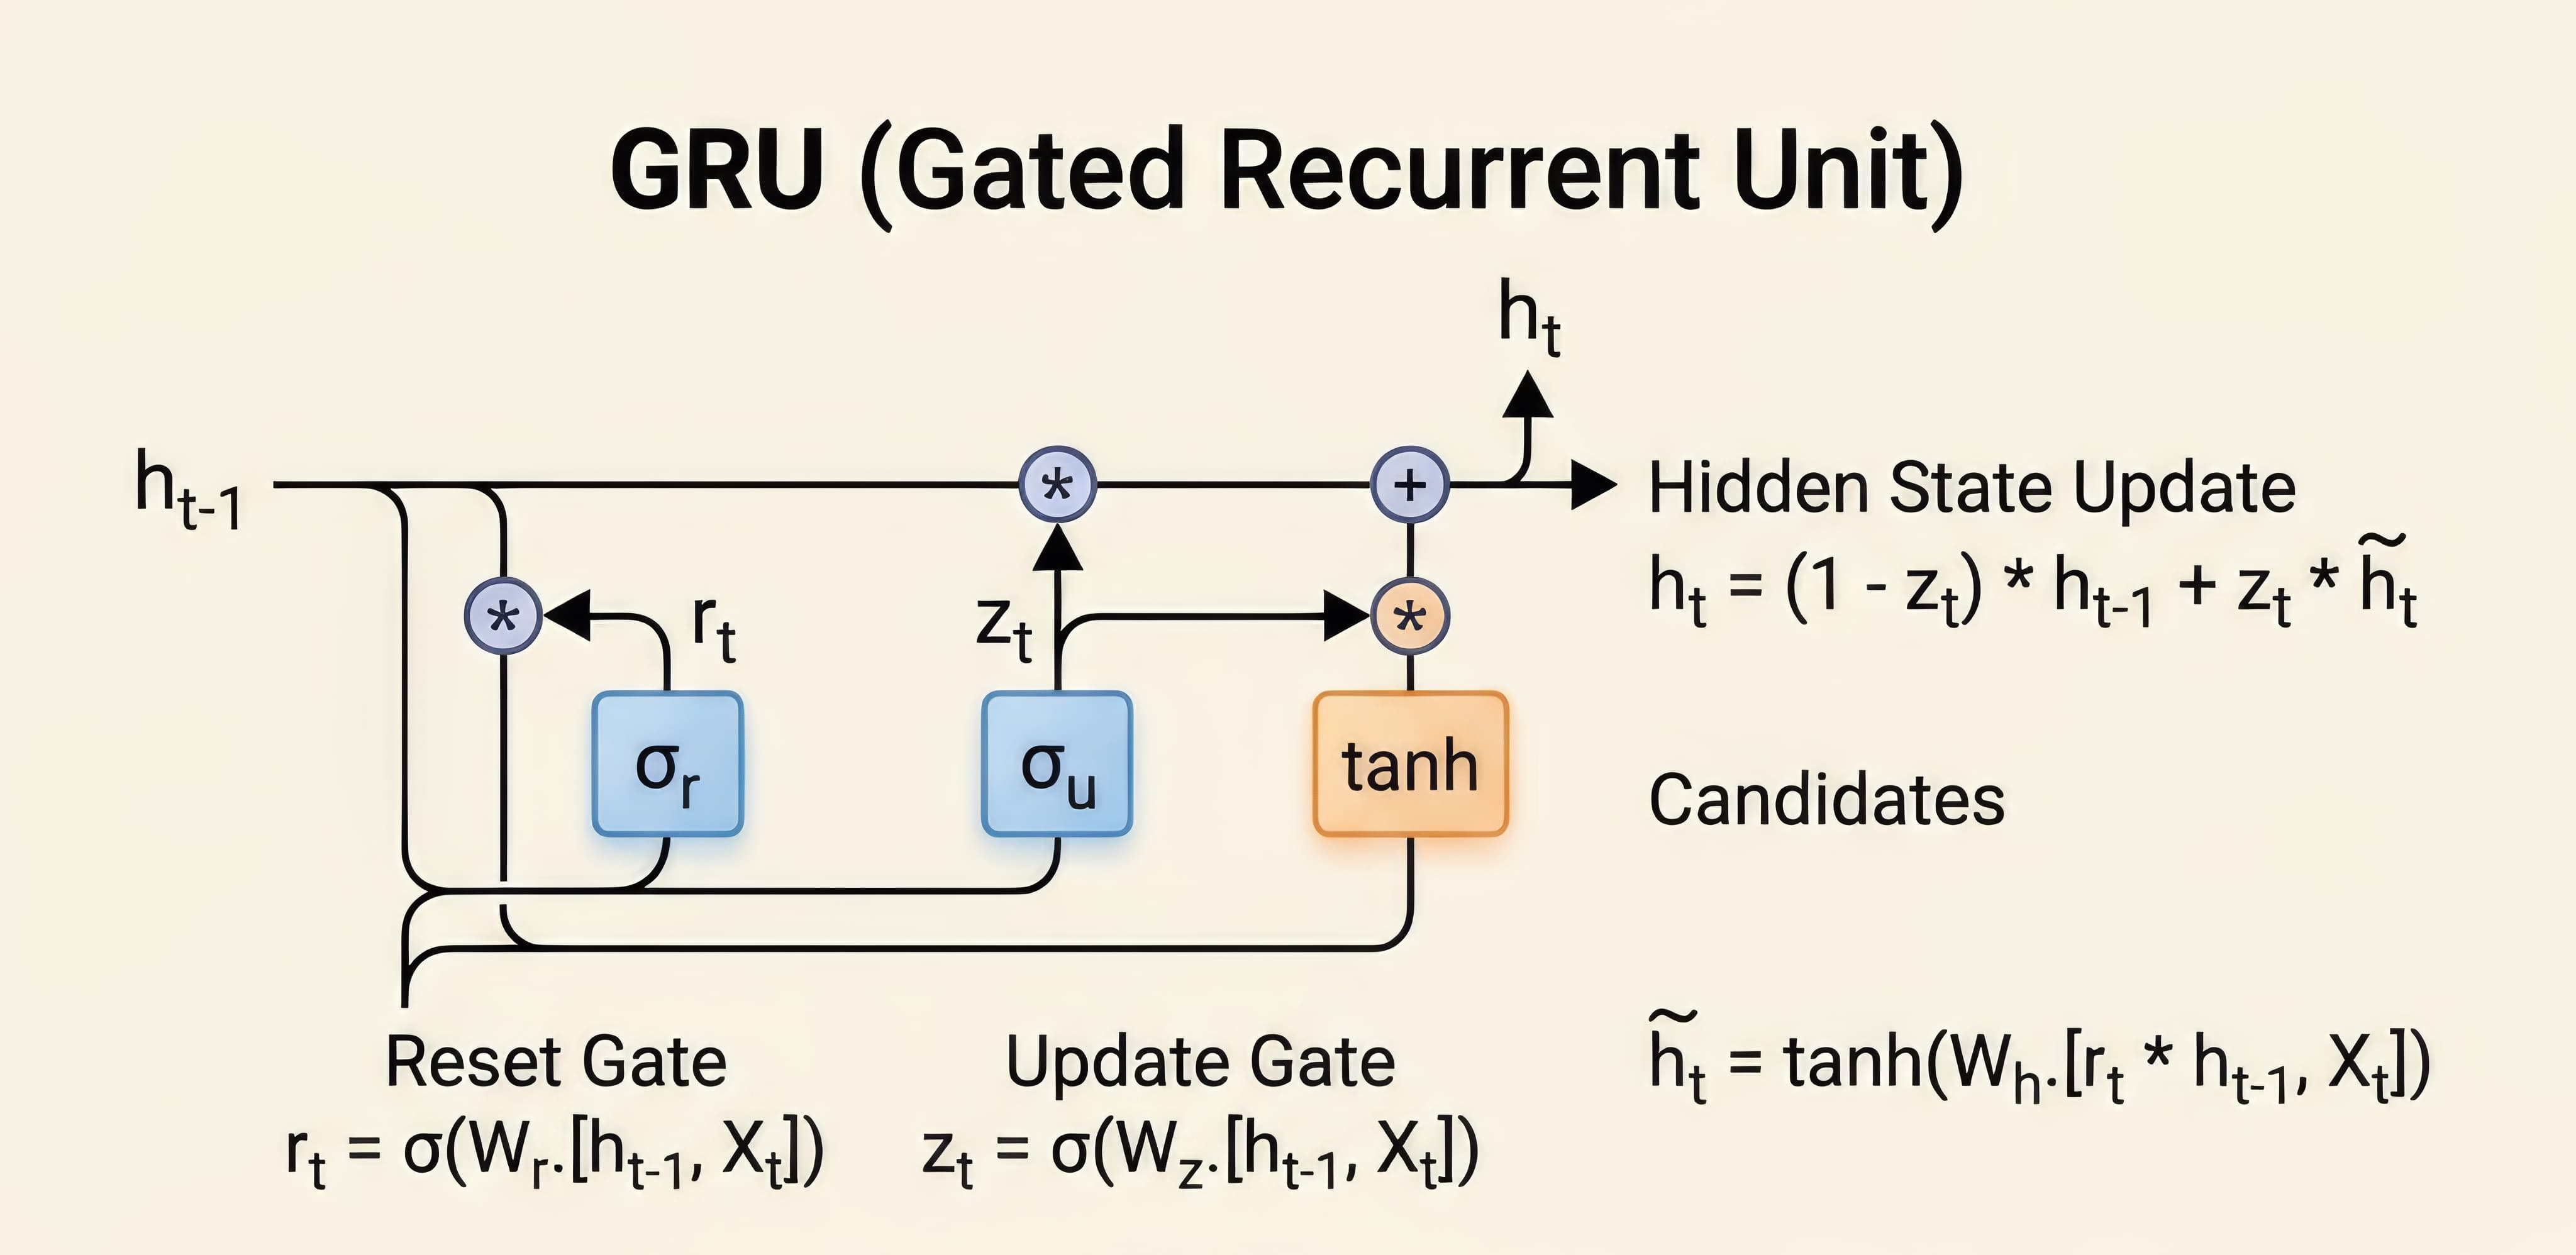
\includegraphics[width=0.8\textwidth]{images/GRU.jpg}
    \caption{Cấu trúc của GRU.}
\end{figure}

GRU là một kiến trúc mạng hồi tiếp được thiết kế để xử lý dữ liệu có cấu trúc chuỗi. Trong mô hình dùng cho IDS, vector đặc trưng có thể được tổ chức lại thành một chuỗi, trong đó mỗi đặc trưng được xem như một bước đầu vào. Cách nhìn này cho phép mô hình đọc dữ liệu tuần tự và duy trì một trạng thái ẩn trong quá trình đọc. Trạng thái ẩn đóng vai trò như bộ nhớ tóm tắt những gì mô hình đã thấy ở các bước trước.
\bigbreak\noindent
Điểm cốt lõi của GRU nằm ở hai cổng: cổng cập nhật (update gate) và cổng đặt lại (reset gate). Cổng cập nhật quyết định bao nhiêu thông tin cũ trong trạng thái ẩn cần được giữ lại khi đọc bước mới. Nếu thông tin cũ vẫn hữu ích, cổng này giữ bộ nhớ ổn định. Nếu bước mới mang tín hiệu quan trọng hơn, cổng cho phép trạng thái thay đổi mạnh hơn. Cổng đặt lại quyết định phần nào của trạng thái cũ nên được quên khi tính ứng viên trạng thái mới. Nhờ hai cổng này, GRU có thể cân bằng giữa ghi nhớ và cập nhật, tránh việc mọi bước đầu vào đều làm mất thông tin trước đó.
\bigbreak\noindent
Trong lan truyền xuôi, mẫu IDS đi qua các lớp GRU theo từng bước. Lớp GRU đầu tạo một chuỗi trạng thái ẩn, mỗi trạng thái phản ánh thông tin đã tích lũy đến vị trí tương ứng. Các lớp GRU tiếp theo tiếp tục đọc chuỗi biểu diễn này để học mẫu phức tạp hơn. Lớp GRU cuối thường trả về trạng thái cuối cùng, xem như bản tóm tắt toàn bộ chuỗi đặc trưng. Bản tóm tắt này đi qua một lớp dense để chuyển thành logits và xác suất lớp sau cùng. Với dữ liệu IDS, GRU có thể học các quan hệ có tính phụ thuộc thứ tự, chẳng hạn một nhóm đặc trưng chỉ có ý nghĩa khi xuất hiện cùng các đặc trưng đứng trước hoặc đứng sau nó.
\bigbreak\noindent
Trong quá trình tinh chỉnh trọng số mô hình, gradient được truyền ngược qua các bước thời gian của GRU. Cơ chế này thường được gọi là backpropagation through time (BPTT). Các cổng của GRU giúp gradient đi qua chuỗi ổn định hơn so với RNN đơn giản, vì mô hình có đường giữ trạng thái cũ và không buộc mọi thông tin phải được viết lại ở mỗi bước. So với LSTM, GRU có ít cổng hơn nên số tham số và chi phí tính toán thường thấp hơn. Điều này làm GRU phù hợp với client có tài nguyên hạn chế trong môi trường học liên kết, nơi mỗi client phải huấn luyện cục bộ nhiều vòng.
\bigbreak\noindent
Đối với dữ liệu IDS dạng bảng, GRU không phải lúc nào cũng vượt trội MLP, vì thứ tự đặc trưng không giống thứ tự thời gian tự nhiên trong văn bản hoặc tín hiệu. Tuy nhiên, GRU vẫn có giá trị khi cách sắp xếp đặc trưng mang thông tin hoặc khi muốn kiểm tra lợi ích của biểu diễn tuần tự. Trong ngữ cảnh mô hình không đồng nhất, GRU cũng đóng vai trò một kiến trúc trung gian: phức tạp hơn MLP, có khả năng ghi nhớ trạng thái, nhưng nhẹ hơn các mô hình lai DCNN-BiLSTM sâu hơn.

\subsection{DCNN-BiLSTM}

\begin{figure}[ht]
    \centering
    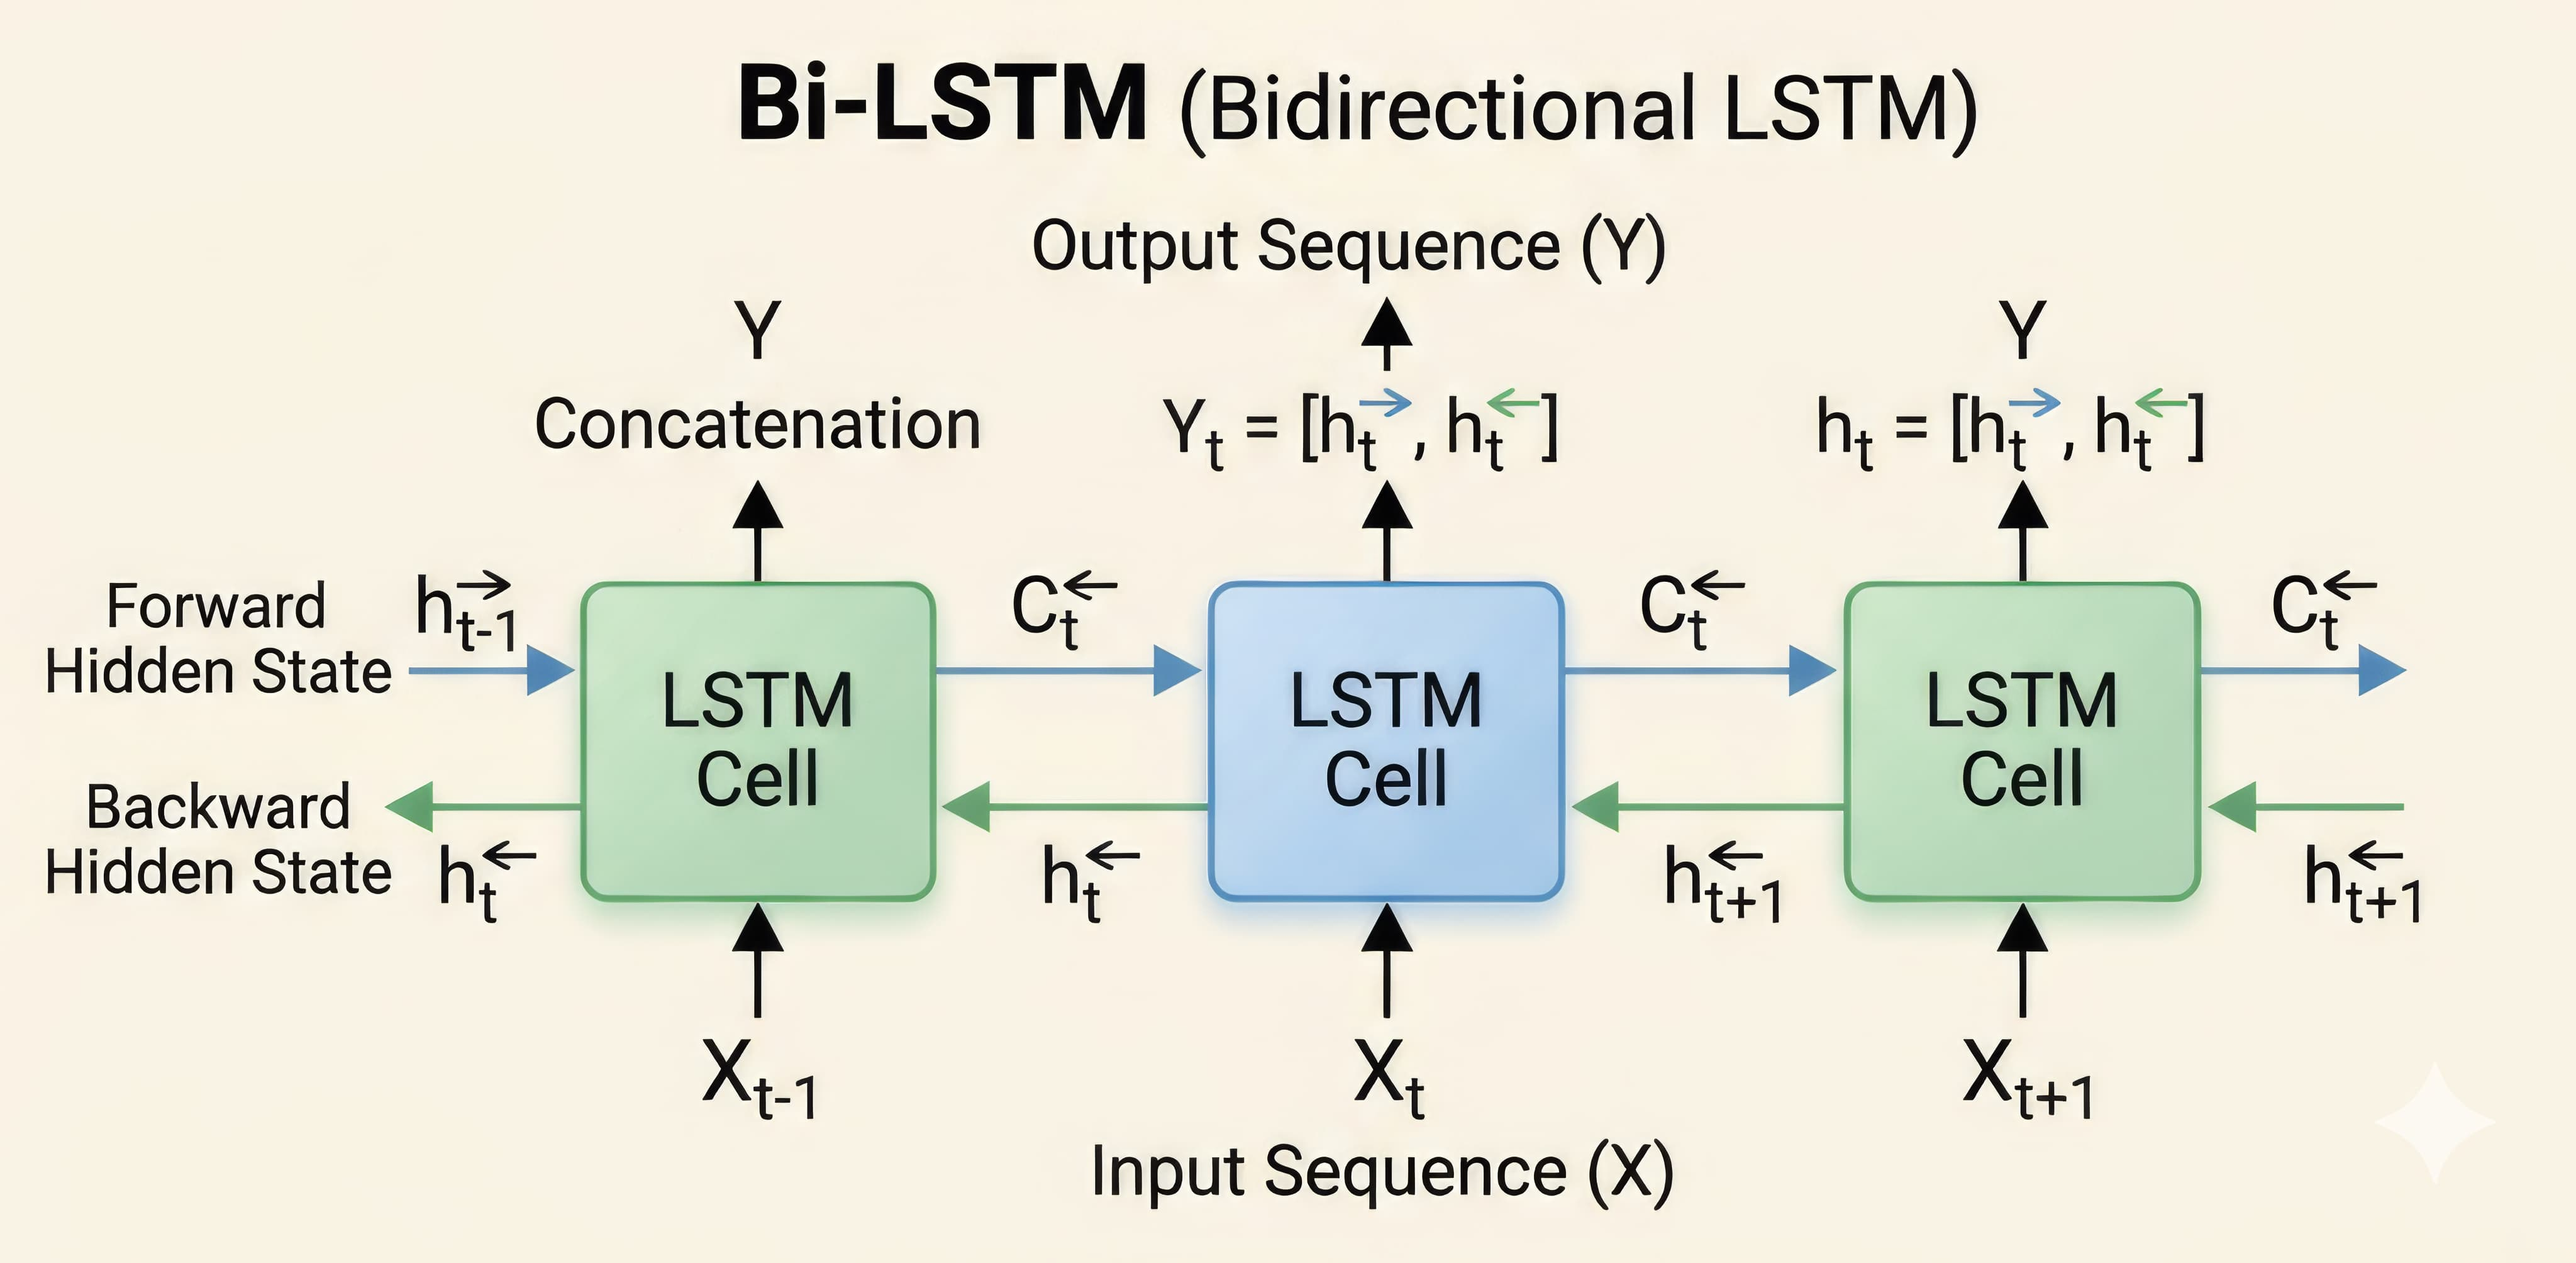
\includegraphics[width=0.9\textwidth]{images/Bi-LSTM.jpg}
    \caption{Cấu trúc của BiLSTM, gồm các cổng điều khiển thông tin.}
\end{figure}

DCNN-BiLSTM kết hợp hai ý tưởng: kiến trúch tích chập để trích xuất mẫu cục bộ và kiến trúc Long-Short Term Memory hai chiều để học phụ thuộc theo hai hướng. Ở phần đầu, dữ liệu đặc trưng được đưa qua lớp Conv1D. Lớp tích chập dùng các bộ lọc trượt trên chuỗi đặc trưng để phát hiện các mẫu cục bộ. Một bộ lọc có thể học rằng một nhóm đặc trưng đứng gần nhau tạo ra tín hiệu hữu ích cho một dạng tấn công. Nhiều bộ lọc khác nhau học nhiều kiểu mẫu khác nhau. Kết quả là mô hình tạo ra một biểu diễn giàu hơn trước khi đưa vào phần hồi tiếp.
\bigbreak\noindent
Sau tích chập, biểu diễn đi vào BiLSTM. LSTM là mạng hồi tiếp có bộ nhớ dài hạn, dùng các cổng để điều khiển thông tin nào được ghi, giữ và xuất ra. BiLSTM chạy LSTM theo hai hướng: một hướng đọc từ đầu đến cuối, hướng còn lại đọc từ cuối về đầu. Hai hướng này được ghép lại để mỗi vị trí trong chuỗi có thông tin từ cả ngữ cảnh trước và sau. Với IDS, cách đọc hai chiều này hữu ích khi ý nghĩa của một đặc trưng phụ thuộc vào cả những đặc trưng đứng trước và đứng sau nó trong biểu diễn đầu vào.
\bigbreak\noindent
Trong lan truyền xuôi, DCNN-BiLSTM hoạt động theo nhiều tầng biểu diễn. Tầng tích chập phát hiện mẫu cục bộ. Tầng BiLSTM thứ nhất giữ chuỗi biểu diễn để học phụ thuộc rộng hơn. Tầng BiLSTM thứ hai nén chuỗi thành một vector ngữ cảnh tổng hợp. Vector này đi qua các lớp dense để tạo biểu diễn phân loại cuối cùng. Layer normalization giúp ổn định biểu diễn, dropout giảm overfitting, còn lớp logits sinh điểm số cho từng lớp.
\bigbreak\noindent
Trong lan truyền ngược, mất mát phân loại truyền gradient qua head dense, qua hai hướng LSTM và về lớp tích chập. Lớp dense học cách dùng biểu diễn tổng hợp để tách lớp. LSTM học cách giữ hoặc quên thông tin theo chuỗi. Lớp tích chập học các bộ lọc cục bộ tốt hơn. Vì nhiều thành phần cùng được cập nhật, DCNN-BiLSTM có năng lực biểu diễn mạnh hơn MLP và GRU. Đổi lại, mô hình có nhiều tham số hơn, chi phí huấn luyện cao hơn và yêu cầu bộ nhớ lớn hơn.
\bigbreak\noindent
Trong bối cảnh IDS, DCNN-BiLSTM phù hợp khi dữ liệu có nhiều tương tác phức tạp và khi hệ thống chấp nhận chi phí tính toán cao để đổi lấy biểu diễn sâu hơn. Trong bối cảnh học liên kết, mô hình này đại diện cho nhóm client mạnh hơn về tài nguyên. Khi đặt cạnh MLP và GRU, nó giúp đánh giá khả năng của các ngữ cảnh mà client không cùng độ phức tạp mô hình. Đây là một điểm quan trọng của học chắt lọc liên kết: các kiến trúc khác nhau vẫn có thể cộng tác thông qua logits hoặc tri thức mềm, thay vì buộc phải có cùng cấu trúc trọng số.

\section{Học máy liên kết}

\subsection{Tổng quan}

Học liên kết là cơ chế huấn luyện phân tán trong đó mỗi client giữ dữ liệu cục bộ và chỉ trao đổi thông tin huấn luyện với server hoặc các client khác. Quy trình cơ bản gồm: server gửi mô hình hiện tại cho client, client huấn luyện cục bộ, client gửi cập nhật, server tổng hợp và phát lại mô hình mới. Mục tiêu là tận dụng dữ liệu phân tán mà không cần chia sẻ dữ liệu thô.

Nếu ký hiệu tham số mô hình ở vòng $t$ là $w^{(t)}$, client $k$ cập nhật $E$ bước với gradient cục bộ $g_k$ thì có thể viết gần đúng
$$
w_k^{(t+1)}=w^{(t)}-\eta\sum_{e=1}^{E} g_{k,e}.
$$
Server sau đó tổng hợp
$$
w^{(t+1)}=\sum_{k=1}^{K}\frac{n_k}{n}w_k^{(t+1)}.
$$

\subsection{FedAvg}

FedAvg là thuật toán nền tảng của học liên kết truyền thống \cite{fedavg}.

FedAvg tổng hợp trọng số mô hình bằng trung bình có trọng số theo số mẫu của client. Đây là thuật toán nền tảng và thường được dùng làm mốc so sánh cho các thuật toán học liên kết khác. Nếu client $k$ có $n_k$ mẫu và tổng số mẫu của các client tham gia là $n=\sum_k n_k$, server cập nhật mô hình toàn cục theo công thức
$$
w^{t+1}=\sum_{k=1}^{K}\frac{n_k}{n}w_k^{t+1}.
$$
Ý nghĩa của công thức này là client có nhiều dữ liệu hơn sẽ đóng góp nhiều hơn vào mô hình toàn cục. Trong môi trường IID, giả định này thường hợp lý vì mỗi client có thể được xem như một mẫu con của cùng một phân phối dữ liệu. Trong môi trường Non-IID, giả định đó yếu đi rõ rệt: một client nhiều mẫu nhưng lệch lớp có thể kéo mô hình toàn cục về phân phối riêng của nó, trong khi một client ít mẫu nhưng chứa lớp hiếm lại có ảnh hưởng nhỏ hơn. Vì vậy, FedAvg đơn giản và hiệu quả, nhưng dễ gặp client drift khi dữ liệu giữa các client không đồng nhất.

\section{Học chắt lọc liên kết}

\subsection{Học chắt lọc}

Chắt lọc tri thức (Knowledge Distillation - KD) \cite{hinton2015kd} là kỹ thuật truyền tri thức từ mô hình này sang mô hình khác thông qua nhãn mềm (soft labels) tính từ phân phối logit và hàm kích họat softmax. Khác với học nhãn cứng như huấn luyện giám sát, mô hình student học phân phối xác suất trong soft labels từ mô hình teacher. Phân phối từ soft labels chứa thông tin về quan hệ giữa các lớp, ví dụ một mẫu có thể rất giống lớp A nhưng cũng gần lớp B hơn các lớp còn lại.

\subsubsection{Temperature và nhãn mềm}

Softmax với temperature $T$ được dùng để làm mềm phân phối xác suất:

$$
p_i = \frac{\exp(z_i / T)}{\sum_j \exp(z_j / T)}.
$$

Khi $T$ lớn hơn, phân phối trở nên mượt hơn và chứa nhiều thông tin hơn về các lớp không phải lớp đúng. Trong chắt lọc tri thức, mô hình học viên thường tối ưu kết hợp giữa mất mát nhãn cứng và mất mát nhãn mềm.

\subsubsection{Chắt lọc bằng Forward Kullback--Leibler}

Phương pháp chắt lọc tri thức được dùng phổ biến nhất dựa trên độ lệch Kullback--Leibler theo chiều thuận giữa hai phân phối softmax: phân phối của mô hình teacher và phân phối của mô hình student. Với logit của giáo viên $z^T$, logit của học viên $z^S$ và temperature $\tau$, hai phân phối mềm được viết là
$$
p_i^T=\frac{\exp(z_i^T/\tau)}{\sum_j\exp(z_j^T/\tau)},
\qquad
p_i^S=\frac{\exp(z_i^S/\tau)}{\sum_j\exp(z_j^S/\tau)}.
$$
Mục tiêu học chắt lọc là làm cho phân phối của student tiến gần phân phối của teacher thông qua mất mát
$$
L_{KD}=\tau^2 KL(p^T\|p^S)=\tau^2\sum_i p_i^T\log\frac{p_i^T}{p_i^S}.
$$
Trong Forward Kullback-Leibler Divergence $KL(p^T\|p^S)$, phân phối giáo viên đuợc đặt ở vai trò tham chiếu, qua đó mô hình student bị phạt thông qua hàm mất mát khi gán xác suất thấp cho những lớp mà mô hình teacher dự đoán khả năng cao. So với mất mát cross-entropy trên nhãn cứng, mục tiêu này truyền thêm "dark knowledge" như quan hệ giữa các lớp: lớp đúng vẫn quan trọng, nhưng các lớp gần với lớp đúng cũng nhận được tín hiệu mềm thay vì bị xem như dự đoán sai trong cross entropy. Trong IDS nhiều lớp, đặc điểm này có ý nghĩa vì nhiều kiểu tấn công có biểu hiện gần nhau, và phân phối mềm giúp mô hình student tiếp nhận cấu trúc trong phân phối mềm mà mô hình teacher đã học được.

\subsubsection{Chắt lọc bằng Evidential Knowledge Distillation}

Evidential Knowledge Distillation (EKD), thay thế phương pháp chắt lọc dựa trên softmax truyền thống là Forward Kullback-Leibler bằng một phân phối Dirichlet trên xác suất lớp \cite{xiang2025ekd,shen2024fdekd}. Với logit $z$, bằng chứng của mô hình được xác định bởi
$$
e=\exp(z),
$$
và tham số Dirichlet được viết là
$$
\alpha=e+\lambda.
$$
Khác với softmax, phép biến đổi theo bằng chứng không loại bỏ hoàn toàn độ lớn tuyệt đối của logit. Tổng nồng độ $\sum_i\alpha_i$ vì vậy trở thành tín hiệu về mức chắc chắn của mô hình: khi bằng chứng lớn và tập trung vào một số lớp, phân phối Dirichlet tập trung tụ lại hơn; khi bằng chứng nhỏ hoặc phân tán, phân phối Dirichlet trải rộng hơn và cho thấy độ bất định cao hơn ở dự đoán của mô hình teacher.

Hàm mất mát của EKD gồm hai thành phần:
$$
L = L_{1st} + \gamma L_{2nd}.
$$
Thành phần thứ nhất căn chỉnh quan hệ tỷ lệ giữa các lớp của học viên và giáo viên:
$$
L_{1st} = KL\!\left(\frac{\alpha_i^T}{\sum_{i \in C}\alpha_i^T} \;\middle\|\; \frac{\alpha_i^S}{\sum_{i \in C}\alpha_i^S}\right).
$$
Thành phần này đóng vai trò chắt lọc ở mức vĩ mô, vì nó tập trung vào hình dạng phân phối lớp sau khi chuẩn hóa. Thành phần thứ hai căn chỉnh toàn bộ phân phối Dirichlet:
$$
L_{2nd} = KL\!\left(Dir(p^T|\alpha^T) \;\middle\|\; Dir(p^S|\alpha^S)\right).
$$
Thành phần này đóng vai trò chắt lọc ở mức vi mô, vì nó giữ lại độ lớn bằng chứng và mức bất định trong phân phối dự đoán của mô hình teacher. Nhờ đó, EKD không chỉ chắt lọc lớp có xác suất cao, mà còn chắt lọc cả mức độ chắc chắn của mô hình khi đưa ra phân phối đó.

\subsubsection{Vai trò trong môi trường liên kết}

Trong học liên kết, chắt lọc tri thức loại bỏ đặc tính đồng nhất kiến trúc. Do các thuật toán học liên kết truyền thống yêu cầu mô hình của các client phải đồng bộ về số chiều để thực hiện tổng hợp, tính thực tiễn của chúng thường bị hạn chế trong các môi trường thực tiễn khi tài nguyên tính toán của mỗi client tham gia rất khác nhau. Mặt khác, chắt lọc kiến thức ban đầu được sử dụng để truyền tải kiến thức giữa các kiến trúc mô hình khác nhau.

Để cho phép các kiến trúc mô hình khác nhau tham gia học liên kết, học máy chắt lọc liên kết chuyển từ tổng hợp trọng số mô hình sang tổng hợp biểu diễn đầu ra của mô hình. Cụ thể hơn, các thuật toán FD sẽ tổng hợp không gian đầu ra như logit vector hoặc prototype theo nhãn, hoặc phân phối dự đoán như logits (có hoặc không có kích hoạt softmax) trên một tập dữ liệu công khai trung gian. Server trong FD sẽ tổng hợp các biểu diễn này và bộ biểu diễn tổng hợp thường được gọi là consensus sẽ đóng vai trò teacher, và mỗi mô hình client sẽ là mô hình student. Thông qua chắt lọc kiến thức từ consensus, FD đạt được tính liên kết giữa các kiến trúc mô hình khác nhau. Điều này đặc biệt phù hợp với IDS vì các tổ chức có thể triển khai mô hình khác nhau tùy tài nguyên và yêu cầu vận hành.

\subsection{FD}

FederatedDistillation \cite{jeong2018federateddistillation} là thuật toán FL tiêu biểu vì thuật toán này dùng nhãn mềm để thay thế cho trao đổi trọng số. Cụ thể, ở mỗi client, mô hình học giám sát và tích lũy soft labels cho từng lớp thành một vector nhãn mềm đại diện cho từng lớp đó $p_{k,c} \leftarrow \frac{1}{|D_{k,c}|\sum_{x \in D_{k,c}}p_k(x)}$. Sau đó, server cộng các vector nhãn mềm này $\bar p_{c} \leftarrow \sum_{k \in K} p_{k,c}$ và mỗi client tự cập nhật mục tiêu chắt lọc bằng cách lấy trung bình bỏ qua chính nó (leave-one-out average):
$$
\bar p_{k,c}=\frac{1}{K-1} (\bar p_c - p_{k,c})
$$

Sau đó, client cập nhật thông qua hàm mất mát chắt lọc. Với mỗi mẫu x thuộc lớp $c$, client tối ưu

$$
L_{FD} = L_{CE} + \lambda KL(\bar p_{k,c} \| p_k(x)).
$$
Với cách này, client không chỉ tự củng cố lại tri thức của chính nó, mà nhận được tín hiệu từ các miền dữ liệu khác. Nếu mục tiêu chắt lọc chứa cả dự đoán của chính client đang học, tín hiệu chung có thể bị kéo về tri thức cục bộ và làm giảm ý nghĩa của việc học liên kết. Leave-one-out average vì vậy làm rõ vai trò của tri thức liên client: mỗi client học từ phần đồng thuận mà các client khác quan sát được trên cùng không gian lớp.

\subsection{FedMD}

FedMD \cite{li2019fedmd} là một thuật toán tiêu biểu khác của hệ thống học chắt lọc liên kết dùng dữ liệu công khai. Ở bước tiền liên kết, mỗi client huấn luyện giám sátn mô hình cục bộ trên tập công khai đã gán nhãn $\{x_p, y_p\} \in D_p$. Sau đó, hệ thống tiến vào giai đoạn học liên kết. Ở mỗi vòng liên kết, client tiếp tục học trên dữ liệu riêng, sau đó dự đoán logit (chưa qua hàm softmax) trên tập công khai, gửi logits tới server để tổng hợp, rồi dùng logit tổng hợp (consensus) này làm mục tiêu chắt lọc:

$$
L_{FedMD} = L_{CE} + \lambda KL(z_{p} \| z_k(x)).
$$

\section{Học liên kết phi tập trung}

\subsection{Động cơ phi tập trung}

Trong học liên kết truyền thống, server trung tâm giữ vai trò điều phối: chọn client, nhận cập nhật của các client tham gia, tổng hợp cập nhật và broadcast kết quả tổng hợp. Cấu trúc này đơn giản nhưng tạo ra một điểm phụ thuộc lớn. Nếu server bị quá tải, bị gián đoạn hoặc không được tất cả tổ chức tin cậy, toàn bộ quá trình học liên kết sẽ bị ảnh hưởng tiêu cực. Học liên kết phi tập trung thay đổi giả định này bằng cách cho phép các client tự điều phối quá trình tổng hợp với nhau mà không cần dựa vào một phần tử cố định.

\subsection{Cơ chế trao đổi trong môi trường phi tập trung}

Nếu ký hiệu $\mathcal{N}(k)$ là tập neighbor (các client kề cạnh trong communication graph) của client $k$, một dạng cập nhật phi tập trung có thể viết là
$$
w_k^{(t+1)}=\sum_{j\in\mathcal{N}(k)}a_{kj}w_j^{(t)},
\qquad \sum_{j\in\mathcal{N}(k)}a_{kj}=1.
$$
Công thức này cho thấy mỗi client tự tổng hợp mô hình mới bằng cách hợp nhất tri thức từ các láng giềng thay vì phải chờ tổng hợp một mô hình toàn cục duy nhất. Khi kết hợp với chắt lọc tri thức, đối tượng trao đổi không nhất thiết là trọng số mô hình $w_j$, mà có thể là logit vector, soft label, prototype hoặc bộ dự đoán trên dữ liệu công khai. Nhờ vậy, thiết kế phi tập trung và chắt lọc tri thức bổ sung cho nhau: phi tập trung cho phép tổng hợp không dựa vào một server, còn chắt lọc kiến thức cho phép tổng hợp kiến thức của nhiều kiến trúc mô hình khác nhau.

\section{Học liên kết tích hợp học tiệm tiến}

\subsection{Học tiệm tiến theo nhãn}

CIL theo dõi khả năng học thêm lớp mới mà vẫn giữ được tri thức cũ. Phần này tập trung vào các thuật toán CIL được dùng làm cơ sở để so sánh với phương pháp đề xuất.

\subsubsection{Bài toán}

CIL mô tả tình huống mô hình học dữ liệu theo từng tác vụ (task), mỗi task $\mathcal{T}$ chứa một tập lớp mới $C^{\mathcal{T}}$. Sau $T$ task, mô hình phải phân loại trên hợp lớp $C^{1:T}=\bigcup_{\mathcal{T}=1}^{T}C^{\mathcal{T}}$ thay vì chỉ phân loại trên lớp mới. Ở task $\mathcal{T}$, dữ liệu đầy đủ của các task trước thường không còn truy cập được, nên mô hình phải học lớp mới trong khi vẫn giữ ranh giới quyết định cho lớp cũ.

Thách thức của CIL là hiện tượng catastrophic forgetting, khi tối ưu theo dữ liệu mới làm tham số rời khỏi vùng từng biểu diễn tốt cho dữ liệu cũ. Có thể nhìn mục tiêu lý tưởng của CIL là tối ưu trên toàn bộ dữ liệu đã từng xuất hiện,
$$
L_{1:T}(w)=\sum_{\mathcal{T}=1}^{T}L_{\mathcal{T}}(w),
$$
nhưng tại thời điểm học task $T$, phần lớn $L_1, L_2, \ldots, L_{T-1}$ không còn được quan sát trực tiếp. Vì vậy, các thuật toán CIL khác nhau chủ yếu khác nhau ở cách giải quyết vấn đề catastrophic forgetting: dùng mô hình cũ làm mô hình teacher và chắt lọc kiến thức task cũ cho mô hình mới, ràng buộc tham số quan trọng, lưu mẫu tái diễn huấn luyện (exemplar), hoặc mở rộng kiến trúc để mô hình thích nghi với lớp mới xuất hiện. Học tiệm tiến theo nhãn như vậy được phân biệt ra $3$ hướng tiếp cận: ràng buộc mô hình thông qua trọng số quan trọng hoặc chắt lọc đầu ra (regularization), tái diễn dữ liệu (exemplar rehearsal/replay) hoặc kiến trúc thích nghi (dynamic architecture). Các hướng này khác nhau ở hàm mất mát, tài nguyên tính toán cũng như yêu cầu về việc biết trước số lượng nhãn.

\subsubsection{Finetune}

Finetune (tối ưu mô hình qua học giám sát) là đường cơ sở cơ bản nhất cho bài toán CIL. Ở task $\mathcal{T}$, mô hình chỉ tối ưu hàm mất mát cross-entropy trên dữ liệu mới:
$$
L_{FT}=L_{CE}(y,p_w(x)),\qquad (x,y)\in D^{\mathcal{T}}.
$$
Không có hạng tử nào ràng buộc trọng số quan trọng, cũng không có bộ nhớ exemplar hoặc mô hình teacher để giúp mô hình mới lưu giữ kiến thức phân loại lớp cũ. Vì vậy, gradient của lớp mới trực tiếp kéo bộ trích xuất đặc trưng (feature extractor) và bộ phân loại (classifier head) về phía phân phối hiện tại. Nếu lớp mới chiếm toàn bộ mini-batch, toàn bộ trọng số mô hình sẽ thay đổi để mang lại hiệu quả phân loại tốt nhất chỉ trên tập lớp mới này. Kết quả là finetune chỉ phân loại tốt trong task mới nhưng thường quên hoàn toàn khả năng phân loại lớp cũ, nên Finetune đóng vai trò cận dưới của bài toán CIL. Trong IDS, đường cơ sở này phản ánh tình huống hệ thống chỉ cập nhật theo kiểu tấn công mới mà không có cơ chế bảo toàn tri thức về những kiểu tấn công đã biết.

\subsubsection{Học tiệm tiến dựa trên ràng buộc mô hình}

\paragraph{Learning without Forgetting - LWF}

\cite{li2017lwf} dùng mô hình cũ làm mô hình teacher để ràng buộc đầu ra của mô hình mới (student) trên các lớp đã học. Ở mỗi task $\mathcal{T}$ và mô hình cũ $w^{old}$, LwF tryền dữ liệu mới đi qua mô hình cũ và mô hình mới, phân phối mềm trên lớp cũ được so khớp bằng chắt lọc tri thức:
$$
L_{LwF}=L_{CE}(y,p_w(x))+
\lambda\tau^2 KL(p_{w^{old}}^{\tau}(x)\|p_w^{\tau}(x)).
$$
Hạng tử đầu học lớp mới bằng nhãn cứng, còn hạng tử thứ hai buộc mô hình mới giữ phản ứng gần với mô hình cũ. Điểm mạnh của LwF là không cần lưu mẫu cũ, nên phù hợp với bối cảnh tài nguyên lưu trữ hạn chế. Tuy nhiên, vì dữ liệu dùng để chắt lọc vẫn là dữ liệu task mới, mô hình cũ chỉ cung cấp tín hiệu cũ thông qua cách nó phản ứng trên mẫu mới. Nếu mẫu mới nằm xa phân phối cũ, phân phối mềm của giáo viên có thể nghèo thông tin và biểu diễn phân phối dự đoán bị sai. Trong IDS, hạn chế này xuất hiện khi kiểu tấn công mới có đặc trưng rất khác các kiểu cũ: mô hình cũ vẫn sinh xác suất trên lớp cũ trong phân phối mềm, nhưng các xác suất đó không đảm bảo đủ tín hiệu để ràng buộc mô hình mới.

\paragraph{Elastic Weight Consolidation - EWC và Memory Aware Synapses - MAS} thuộc nhóm ràng buộc tham số \cite{kirkpatrick2017ewc,aljundi2018mas}. Thay vì lưu mẫu của lớp cũ, nhóm phương pháp này giả định rằng không phải mọi tham số đều quan trọng như nhau đối với tri thức cũ. Nếu một tham số có ảnh hưởng lớn đến phân loại lớp cũ, EWC và MAS ràng buộc thay đổi của nhóm tham số này.

EWC xấp xỉ ảnh hưởng của mất mát cũ quanh nghiệm $w^*$ bằng khai triển bậc hai. Với ma trận Fisher $F_i$, mục tiêu ở task CIL mới được viết là
$$
L_{EWC}=L_{\mathcal{T}}(w)+\frac{\lambda}{2}\sum_i F_i(w_i-w_i^*)^2.
$$
Ở đây $F_i$ đo độ nhạy của log-likelihood cũ theo tham số $w_i$. Nếu $F_i$ lớn, bất cứ thay đổi nào lên tham số đó sẽ bị phạt qua hàm mất mát; nếu $F_i$ nhỏ, biến đổi trên các tham số đó sẽ tạo ra mất mát ít hơn, cho phép mô hình thích nghi nhiều hơn với task mới. Việc điều chỉnh trọng số của hạng tử Fisher $\lambda$ cho góc nhìn rõ ràng hơn về hạn chế stability và plasticity của các phương pháp ràng buộc trọng số: stability đến từ việc giữ tham số quan trọng, còn plasticity đến từ việc vẫn cho phép tham số ít quan trọng học lớp mới, và các siêu tham số như $\lambda$ buộc phải đánh đổi giữa cả hai, từ đó tạo ra hạn chế yêu cầu việc tinh chỉnh tham số trong thực tế.

MAS cũng ràng buộc các thay đổi tham số, nhưng không ước lượng độ quan trọng của tham số dựa trên nhãn hay Fisher information. Phương pháp này đo độ nhạy của chuẩn đầu ra theo tham số:
$$
\Omega_i=\frac{1}{N}\sum_{x}\left\|\frac{\partial \|f(x;w)\|_2^2}{\partial w_i}\right\|.
$$
Mục tiêu học sau đó có dạng
$$
L_{MAS}=L_{\mathcal{T}}(w)+\lambda\sum_i \Omega_i(w_i-w_i^*)^2.
$$
Vì không cần nhãn để ước lượng $\Omega_i$ mà chỉ cần dựa vào thay đổi đầu ra của mô hình, MAS phù hợp hơn khi dữ liệu không được gán nhãn đầy đủ. Trong IDS, hai phương pháp này hữu ích khi không muốn tốn kém chi phí lưu trữ mẫu huấn luyện cũ, nhưng chúng có thể làm mô hình kém linh hoạt nếu kiểu tấn công mới đòi hỏi thay đổi mạnh ở cùng các tham số từng quan trọng cho lớp cũ.

\paragraph{Prototype augmentation and self-supervision for incremental learning - PASS} \cite{zhu2021pass} là phương pháp không dùng exemplar, dựa trên prototype augmentation và self-supervision. Thay vì lưu mẫu cũ, PASS duy trì các prototype của lớp cũ trong không gian đặc trưng. Từ prototype $\phi_c$, phương pháp tạo các đặc trưng giả quanh tâm lớp để mô phỏng vùng dữ liệu cũ:
$$
\tilde \phi_c=\phi_c+\epsilon,\qquad \epsilon\sim\mathcal{N}(0,\sigma_c^2 I).
$$
Các đặc trưng giả này  giúp lớp phân loại của mô hình (classifier head) tiếp tục nhìn thấy tín hiệu của lớp cũ khi học lớp mới. Vì vậy, PASS củng cố decision boundary bằng cách tái tạo vùng lân cận của prototype task cũ thay vì tái tạo mẫu đầu vào. Ngoài ra, tương tự với LwF, PASS hạn chế catastrophic forgetting bằng cách chắt lọc đầu ra của feature extractor cũ cho feature extractor mới ở task mới. Hàm mất mát của PASS như sau:

$$
L_{total} = L_{CE} + \lambda KL(p_{old}(x)\|p_{new}(x)) + \gamma L_{protoAug}.
$$

Trong đó, $\lambda$ và $\gamma$ là hệ số điều chỉnh cho hạng tử chắt lọc và hạng tử huấn luyện classifier head từ đặc trưng giả. $L_{protoAug}$ là hàm mất mát của huấn luyện phân loại các đặc trưng giả $\tilde \phi_c$ vào lớp $c$:

$$
L_{protoAug} = \sum_c L_{CE}(f_{classifier}(\tilde \phi_c), y_c).
$$

trong đó, $f_{classifier}$ là lớp phân loại (classifier head) của mô hình chính $f$, và $f_{classifier}(\tilde \phi_c)$ là đầu ra của lớp phân loại cho đặc trưng giả lớp $c$, còn $y_c$ là nhãn của lớp $c$.

PASS tạo ra một cơ chế chống quên không cần huấn luyện tái diễn: nó không lưu dữ luyện huấn luyện cũ, nhưng vẫn giữ được ước lượng hình học (thông qua prototype) của các lớp đã học.

\paragraph{Correlation-based Knowledge Distillation in Exemplar-Free Class-Incremental Learning - CBKD EFCIL} \cite{gao2025cbkdefcil}. Tương tự như PASS, CBKD EFCIL thuộc nhóm exemplar-free (EF CIL), nghĩa là phương pháp này không lưu mẫu huấn luyện cũ khi chuyển sang task mới. Thay vào đó, CBKD giữ một mô hình cũ làm teacher, một mô hình hiện tại làm student và duy trì prototype của từng lớp trong không gian đặc trưng. Điểm khác biệt chính so với LwF nằm ở cách ràng buộc đầu ra: thay vì chỉ ép hai phân phối xác suất gần nhau bằng KL, CBKD đo mức tương quan giữa phản ứng của mô hình cũ và mô hình mới trên các lớp đã học. Nếu hai vector dự đoán giữ cùng quan hệ tăng giảm giữa các lớp cũ, mô hình mới được xem là còn bảo toàn cấu trúc tri thức cũ tốt hơn, ngay cả khi giá trị logit tuyệt đối đã thay đổi trong quá trình học lớp mới.

Với một mẫu $x$, ký hiệu $\hat q(x)$ là dự đoán của mô hình cũ trên $O$ lớp đã học và $q(x)$ là phần dự đoán tương ứng của mô hình mới. Tương quan Pearson giữa hai vector được tính theo công thức
$$
\rho_{Pearson}(\hat q(x),q(x))=
\frac{\sum_{c=1}^{O}(\hat q_c(x)-\bar{\hat q}(x))(q_c(x)-\bar q(x))}
{\sqrt{\sum_{c=1}^{O}(\hat q_c(x)-\bar{\hat q}(x))^2
\sum_{c=1}^{O}(q_c(x)-\bar q(x))^2}}.
$$
Từ đó, khoảng cách Pearson được viết là
$$
d_{Pearson}(\hat q(x),q(x))=1-\rho_{Pearson}(\hat q(x),q(x)).
$$
Khi hai vector có quan hệ tuyến tính gần nhau, khoảng cách này nhỏ; khi quan hệ giữa các lớp bị đảo hoặc mất tương quan, khoảng cách tăng lên. Vì vậy, hạng tử chắt lọc của CBKD không chỉ giữ xác suất của từng lớp riêng lẻ, mà còn dựa vào tương quan giữa các lớp cũ trong dự đoán của các mô hình (correlation-based).

Với một batch $\mathcal{B}$ gồm $|\mathcal{B}|$ mẫu, CBKD xây dựng hai thành phần tương quan. Thành phần inter-class đo khoảng cách Pearson theo từng mẫu:
$$
L_{inter}=\frac{1}{|\mathcal{B}|}\sum_{i=1}^{|\mathcal{B}|}d_{Pearson}(\hat p_i,p_i),
$$
trong đó $\hat p_i$ và $p_i$ là vector dự đoán trên các lớp cũ của mẫu thứ $i$ từ teacher và student. Thành phần intra-class đo khoảng cách Pearson theo từng lớp cũ trên toàn batch:
$$
L_{intra}=\frac{1}{O}\sum_{j=1}^{O}d_{Pearson}(\hat p^j,p^j),
$$
trong đó $\hat p^j$ và $p^j$ là cột dự đoán của lớp cũ thứ $j$ qua các mẫu trong batch. Hai thành phần này được kết hợp thành mất mát correlation-based feature distillation:
$$
L_{CFD}=\alpha L_{inter}+\beta L_{intra}.
$$
$L_{inter}$ giữ quan hệ giữa các lớp trong từng mẫu, còn $L_{intra}$ giữ cách một lớp cũ phản ứng trên nhiều mẫu khác nhau. Cách kết hợp này phù hợp với CIL vì mô hình mới cần học lớp mới, nhưng vẫn không nên phá vỡ mẫu phản ứng mà mô hình cũ đã học cho các lớp trước.

Bên cạnh chắt lọc tương quan, CBKD duy trì prototype lớp để thay thế cho exemplar. Sau mỗi task, với lớp $c$, prototype được tính bằng trung bình đặc trưng của các mẫu thuộc lớp đó:
$$
\mu_c=\frac{1}{|\mathcal{B}_c|}\sum_{i=1}^{|\mathcal{B}_c|}F(x_i;\theta),
$$
trong đó $F(x_i;\theta)$ là đầu ra của bộ trích xuất đặc trưng và $|\mathcal{B}_c|$ là số mẫu của lớp $c$. Độ phân tán chung của đặc trưng được biểu diễn bằng phương sai $r^2$, tính từ trace của ma trận covariance theo đặc trưng của từng lớp:
$$
r_t^2=\frac{1}{M_{old}+M_{new}}\left(M_{old}r_{t-1}^2+
\sum_{c\in C_t}\frac{\operatorname{Tr}(\Sigma_{t,c})}{D_{proto}}\right),
$$
trong đó $M_{old}$ và $M_{new}$ lần lượt là số lớp cũ được giữ prototype và số lớp mới ở task hiện tại, $C_t$ là tập lớp xuất hiện ở task $t$, $D_{proto}$ là chiều không gian đặc trưng và $\Sigma_{t,c}$ là ma trận covariance của đặc trưng lớp $c$. Từ prototype đã lưu, phương pháp tạo đặc trưng giả bằng nhiễu Gaussian
$$
\xi_c=\mu_c+g r, \qquad g\sim\mathcal{N}(0,I),
$$
rồi đưa $\xi_c$ qua classifier head để huấn luyện phân loại lớp cũ:
$$
L_{proto}=\sum_{c=1}^{O}L_{CE}(C_\phi(\xi_c),y_c).
$$
Như vậy, classifier vẫn tiếp tục nhận tín hiệu về lớp cũ mà không cần lưu exemplar.

Tổng mất mát của CBKD ở các task sau được viết là
$$
L_{CBKD}=L_{CE}+L_{CFD}+\lambda L_{proto}.
$$
Ở task đầu tiên, mô hình chưa có lớp cũ nên chỉ học giám sát và sau đó ghi nhận prototype cho các lớp đã thấy. Từ task thứ hai trở đi, mô hình cũ từ giai đoạn trước cung cấp tín hiệu tương quan trên lớp cũ, còn prototype cục bộ cung cấp dữ liệu đặc trưng giả cho classifier.

\subsubsection{Học tiệm tiến dựa trên tái diễn dữ liệu}

\paragraph{Incremental Classifier and representation learning - iCaRL và Bias Correction - BiC} lưu mẫu exemplar đại diện cho lớp cũ và kết hợp tái diễn dữ liệu (replay) với chắt lọc tri thức \cite{rebuffi2017icarl}. Trong iCaRL, với mỗi lớp $c\in C$, một tập mẫu nhỏ $D^{exemplar}_c$ được chọn sao cho trung bình đặc trưng của exemplar gần trung bình đặc trưng của toàn lớp:
$$
\mu_c=\frac{1}{|D_c|}\sum_{x\in D_c}\phi(x),
\qquad
D^{exemplar}_c\approx \arg\min_D\left\|\mu_c-\frac{1}{|D|}\sum_{x\in D}\phi(x)\right\|.
$$
Khi suy luận, iCaRL dùng nguyên tắc nearest-mean-of-exemplars: mẫu được gán vào lớp có trung bình exemplar gần nhất trong không gian đặc trưng. Trong huấn luyện, exemplar của lớp cũ được trộn với dữ liệu lớp mới, còn chắt lọc tri thức giữ đầu ra của mô hình mới gần mô hình cũ trên các lớp đã học. Vì vậy, iCaRL giải quyết quên bằng hai neo cùng lúc: neo dữ liệu thông qua exemplar và neo hàm thông qua chắt lọc. BiC \cite{wu2019bic} tập trung vào một vấn đề khác của CIL: thiên lệch (bias) về lớp mới. Khi dữ liệu huấn luyện chứa toàn bộ mẫu lớp mới nhưng chỉ một số exemplar lớp cũ, bộ phân loại thường tạo logit lớn hơn cho lớp mới. BiC thêm một tầng hiệu chỉnh tuyến tính lên logits của các lớp mới:
$$
q_c=\alpha z_c+\beta,\qquad c\in C^{\mathcal{T}},
$$
trong đó $z_c$ là logit ban đầu của lớp $c$, còn $\alpha$ và $\beta$ được học để giảm lệch giữa lớp cũ và lớp mới. Ý nghĩa của BiC không nằm ở việc học thêm đặc trưng mới, mà ở việc sửa thang đo đầu ra sau khi mô hình đã học trên dữ liệu mất cân bằng. Trong IDS, cơ chế này quan trọng vì dữ liệu về kiểu tấn công mới thường nhiều hơn trong giai đoạn cập nhật, trong khi các kiểu cũ chỉ còn một số mẫu đại diện hoặc thống kê tóm tắt.

\subsubsection{Học tiệm tiến với kiến trúc dynamic}

Một nghiên cứu tiêu biểu cho nhóm phương pháp này là FOSTER \cite{wang2022foster} dùng cơ chế feature boosting và compression để xử lý mâu thuẫn giữa mở rộng kiến trúc mô hình và giữ kiến trúc mô hình vừa phải để tiết kiệm chi phí tính toán. Ở giai đoạn boosting, mô hình được mở rộng bằng một nhánh biểu diễn mới để học các lớp vừa xuất hiện, trong khi nhánh cũ giữ tri thức đã có. Nếu ký hiệu đặc trưng cũ là $f_{old}(x)$ và đặc trưng mới là $f_{new}(x)$, biểu diễn dùng cho phân loại có thể nhìn như phép ghép
$$
f_{boost}(x)=[f_{old}(x);f_{new}(x)].
$$
Cách ghép này tăng dung lượng biểu diễn, giúp mô hình không phải ép toàn bộ lớp mới vào không gian đặc trưng cũ vốn đã được tổ chức cho các lớp trước. Nhờ vậy, FOSTER giảm áp lực làm biến dạng biểu diễn cũ khi học lớp mới.

Tuy nhiên, nếu cứ mở rộng sau mỗi task, kích thước mô hình sẽ tăng liên tục. Vì vậy, FOSTER dùng giai đoạn compression để nén mô hình mở rộng về một mô hình nhỏ hơn bằng chắt lọc tri thức. Mô hình nén học từ đầu ra hoặc đặc trưng của mô hình đã boost:
$$
L_{comp}=L_{CE}+\lambda KL(p_{boost}^{\tau}\|p_{compact}^{\tau}).
$$
Hai giai đoạn này tách rõ hai nhu cầu của CIL: trước hết cần đủ năng lực để hấp thụ lớp mới, sau đó cần đưa tri thức về một mô hình ổn định để tiếp tục học ở task sau. Trong IDS, FOSTER phù hợp với bối cảnh số lớp tấn công tăng dần, nhưng không thể để mô hình triển khai phình to không kiểm soát sau mỗi lần cập nhật.

% \subsection{Global-Local Forgetting Compensation (GLFC)}

% GLFC \cite{dong2022glfc} là phương pháp FCIL kết hợp bốn cơ chế: exemplar replay, gradient compensating, chắt lọc quan hệ, và lựa chọn mô hình toàn cục tốt nhất qua proxy server. Phương pháp xử lý đồng thời hai nguồn lệch: lệch lớp theo thời gian và Non-IID giữa các client.

% \textbf{Exemplar replay theo herding.}
% Mỗi client $k$ duy trì tập exemplar riêng với ngân sách bộ nhớ $M$ được chia đều cho tất cả các lớp đã quan sát. Exemplar được chọn theo phương pháp herding của iCaRL: với mỗi lớp $c$, đặc trưng của từng mẫu được chuẩn hóa, sau đó các mẫu được chọn tuần tự sao cho trung bình tích lũy của tập đã chọn xấp xỉ gần nhất với trung bình toàn lớp. Khi sang task mới, tập exemplar cũ được thu hẹp để duy trì ngân sách $M$, rồi exemplar cho lớp mới được bổ sung vào. Dữ liệu huấn luyện mỗi vòng gồm mẫu mới lẫn exemplar cũ.

% \textbf{Gradient compensation và relation distillation.}
% Hàm mất mát GLFC gồm hai thành phần. Thành phần thứ nhất, $L_{GC}$, điều chỉnh trọng số per-sample dựa trên sai số dự đoán tại nhãn thật: với mẫu có nhãn $c$, trọng số được tính là $g_i = |\sigma(z_{i,c}) - 1|$, trong đó $z_{i,c}$ là logit tương ứng. Để tránh mất cân bằng giữa nhóm lớp cũ và lớp mới, $g_i$ được chuẩn hóa bằng cách chia cho giá trị trung bình nhóm tương ứng. Thành phần thứ hai, $L_{RD}$, là chắt lọc quan hệ: mô hình cũ tạo ra xác suất sigmoid cho $C_{old}$ lớp đã học, các xác suất này được ghép với nhãn thật của lớp mới để tạo tín hiệu chắt lọc. Tổng hàm mất mát:
% $$
% L_{GLFC} = \tfrac{1}{2}\,L_{GC} + \tfrac{1}{2}\,L_{RD}.
% $$
% Khi chưa có lớp cũ (task đầu tiên), $L_{RD} = 0$ và chỉ có $L_{GC}$ được tối ưu.

% \textbf{Gradient encoder và gradient masking.}
% GLFC tích hợp một cơ chế tùy chọn để hỗ trợ lựa chọn mô hình tốt nhất qua máy chủ trung gian (proxy server). Mỗi client huấn luyện một mạng encoder $E_\theta$ nhỏ (dense hoặc GRU hai lớp với đầu ra $C$ lớp) để mã hóa thông tin prototype lớp. Với mỗi lớp mới $c$, client chọn mẫu trung tâm $\mathbf{x}^*_c$ (mẫu gần nhất với trung bình đặc trưng chuẩn hóa của lớp đó), sau đó tinh chỉnh nhẹ $\mathbf{x}^*_c$ bằng SGD và hàm mất mát sigmoid cross-entropy để tăng cường tính đại diện. Tiếp theo, gradient của $E_\theta$ tại mẫu tinh chỉnh đó được tính và làm thưa bằng cách đặt về 0 tất cả phần tử có giá trị tuyệt đối dưới phân vị thứ 30. Tập gradient có mặt nạ này được gửi đến proxy server thay vì gửi dữ liệu thô, nhờ đó bảo vệ quyền riêng tư.

% \textbf{Tái tạo dữ liệu bằng DLG và lựa chọn mô hình.}
% Proxy server nhận tập gradient $\{G_j\}$ từ các client, suy ra nhãn lớp cho mỗi $G_j$ từ cột có gradient âm lớn nhất trong lớp fully-connected cuối, rồi tái tạo mẫu dữ liệu giả thông qua Deep Leakage from Gradients (DLG) \cite{zhu2019dlg}. Cụ thể, với mỗi gradient $G_j$, một biến $\tilde{\mathbf{x}}$ được khởi tạo ngẫu nhiên và tối ưu bằng Adam để gradient của $E_\theta$ tại $\tilde{\mathbf{x}}$ xấp xỉ $G_j$:
% $$
% \tilde{\mathbf{x}}^* = \arg\min_{\tilde{\mathbf{x}}} \sum_l \bigl\|\nabla_{\theta_l} \mathcal{L}(E_\theta(\tilde{\mathbf{x}}), c_j) - G_j^{(l)}\bigr\|^2.
% $$
% Các mẫu tái tạo được tích lũy thành tập proto-data của proxy server. Sau mỗi vòng tổng hợp, proxy server đánh giá mô hình toàn cục trên tập proto-data này và chỉ lưu lại trọng số của mô hình nào đạt độ chính xác cao nhất. Trước khi bắt đầu task tiếp theo, trọng số tốt nhất đó được dùng để khởi tạo mô hình cũ $f_{old}$ thay vì dùng trọng số từ vòng cuối, giúp $L_{RD}$ chắt lọc từ một mô hình ổn định hơn.

\subsection{Federated Geometry-Aware Correction} \cite{qi2026feat} FEAT là một hệ thống học liên kết tích hợp học tiệm tiến khai thác cấu trúc hình học của không gian đặc trưng thông qua Equiangular Tight Frame (ETF). Khác với các phương pháp dựa vào replay hoặc chắt lọc đầu ra, FEAT thay thế classifier head bằng một ma trận prototype tĩnh có cấu trúc ETF, từ đó kiểm soát hình học của biểu diễn lớp ngay tại tầng cuối.

Giả sử tại task $t$, tập lớp tích lũy là $C_t$ với $|C_t|$ lớp, và bộ trích xuất đặc trưng sinh ra biểu diễn $f(x) \in \mathbb{R}^d$. FEAT xây dựng ma trận ETF $W_t \in \mathbb{R}^{d \times |C_t|}$ sao cho mỗi cột $\phi_c$ là prototype chuẩn hóa của lớp $c$ và thỏa mãn
\[
\phi_i^{\top} \phi_j =
\begin{cases}
1, & i=j,\\
\dfrac{-1}{|C_t|-1}, & i\neq j.
\end{cases}
\]
Cấu trúc này đảm bảo mọi prototype có cùng chuẩn $\ell_2$ và góc giữa hai lớp bất kỳ là đồng đều, nhờ đó giảm bias hình học giữa các lớp cũ và lớp mới.

Logit của mẫu $x$ được tính trực tiếp bằng tích vô hướng
\[
z_c = f(x)^{\top} \phi_c,
\]
và mất mát phân loại được viết là
\[
L_{CLS} = - \sum_{c \in C_t} y_c \log \operatorname{softmax}(f(x)^{\top} \phi_c).
\]
Ở task đầu tiên, $L_{CLS}$ là thành phần duy nhất. Từ task thứ hai trở đi, FEAT bổ sung hạng tử Geometric Structural Alignment (GSA):
\[
L = L_{CLS} + \lambda L_{GSA}.
\]

Với một batch $B \subset D$ có $|B|$ mẫu, ký hiệu $f_a = f(x_a)$ là đặc trưng của mẫu $a$. Ma trận tương đồng đặc trưng được tính bằng cosine similarity
\[
M_F^{a,b} = \frac{\langle f_a, f_b \rangle}{\|f_a\|_2 \|f_b\|_2}.
\]
Ma trận mục tiêu $M_P$ được xây dựng từ các prototype ETF tương ứng với nhãn của từng mẫu:
\[
M_P^{a,b} = \frac{\langle \phi_{y_a}, \phi_{y_b} \rangle}{\|\phi_{y_a}\|_2 \|\phi_{y_b}\|_2}.
\]
Sau khi chuẩn hóa từng hàng bằng softmax để thu được phân phối $P_F^a$ và $P_P^a$, mất mát GSA được tính bằng
\[
L_{GSA} = \frac{1}{|C_{batch}|} \sum_{c \in C_{batch}} \frac{1}{|D_c \cap B|} \sum_{a: y_a = c} KL(P_F^a \| P_P^a).
\]
Hạng tử này buộc cấu trúc tương đồng giữa các mẫu trong không gian đặc trưng tiệm cận cấu trúc simplex đều của ETF. Việc lấy trung bình theo từng lớp trước khi lấy trung bình trên các lớp cũng giúp giảm ảnh hưởng của mất cân bằng lớp trong batch.

Để xử lý drift giữa nhóm lớp mới (head) và lớp cũ (tail), FEAT chia $W_t$ thành hai phần $W_H$ và $W_T$ tương ứng với $C_H$ và $C_T$. Từ đó, hai projector được xây dựng bằng Moore--Penrose pseudoinverse:
\[
P_H = W_H (W_H^{\top} W_H)^{\dagger} W_H^{\top}, \qquad
P_T = W_T (W_T^{\top} W_T)^{\dagger} W_T^{\top}.
\]
Với đặc trưng chuẩn hóa $\tilde f$, năng lượng chiếu được định nghĩa là
\[
e_H(\tilde f) = \frac{\|P_H \tilde f\|_2^2}{|C_H|-1}, \qquad
e_T(\tilde f) = \frac{\|P_T \tilde f\|_2^2}{|C_T|-1}.
\]
Trong giai đoạn exemplar replay, mỗi client $k$ tính trung bình trượt (EMA) của hai năng lượng này trên tập exemplar $D_{k,T}$:
\[
e_{H,k} \leftarrow (1-\rho)e_{H,k} + \rho\frac{1}{|D_{k,T}|}\sum_{x \in D_{k,T}} e_H(\tilde f(x)),
\]
\[
e_{T,k} \leftarrow (1-\rho)e_{T,k} + \rho\frac{1}{|D_{k,T}|}\sum_{x \in D_{k,T}} e_T(\tilde f(x)).
\]
Server tổng hợp theo số mẫu để thu được prior toàn cục
\[
\bar e_H^{(G)} = \frac{\sum_k |D_{k,T}| e_{H,k}}{\sum_k |D_{k,T}|}, \qquad
\bar e_T^{(G)} = \frac{\sum_k |D_{k,T}| e_{T,k}}{\sum_k |D_{k,T}|}.
\]

Ở pha suy luận, với đặc trưng chuẩn hóa $\tilde x$, FEAT xây dựng hệ số điều chỉnh
\[
g(\tilde x) = \max \left\{ \frac{e_H(\tilde x) - \bar e_H^{(G)}}{e_H(\tilde x) + e_T(\tilde x) + \varepsilon}, 0 \right\},
\]
rồi hiệu chỉnh biểu diễn bằng cách giảm thành phần head-aligned và tăng thành phần tail-aligned:
\[
\tilde x' = \tilde x - g(\tilde x) P_H \tilde x + g(\tilde x) P_T \tilde x,
\qquad
\tilde x' \leftarrow \frac{\tilde x'}{\|\tilde x'\|_2}.
\]
Dự đoán cuối cùng được tính bằng ETF similarity:
\[
z_c = (\tilde x')^{\top} \phi_c, \qquad c \in C_t.
\]

% Nhờ cấu trúc ETF và cơ chế hiệu chỉnh dựa trên năng lượng chiếu, FEAT không chỉ duy trì exemplar replay như iCaRL, mà còn kiểm soát hình học của không gian đặc trưng trong suốt quá trình học tiệm tiến liên kết. Điều này phù hợp với FCIL trong IDS, nơi mỗi client có thể quan sát phân phối lớp khác nhau và lớp mới xuất hiện dần theo thời gian.

Nhờ cấu trúc ETF và cơ chế hiệu chỉnh dựa trên năng lượng chiếu, FEAT không đơn thuần là exemplar rehearsal như iCaRL mà còn chủ động bảo toàn cấu trúc hình học của không gian đặc trưng trong suốt quá trình học tiệm tiến liên kết. Điều này đặc biệt phù hợp với bài toán FCIL trong IDS, nơi dữ liệu giữa các client thường không đồng nhất, các lớp tấn công mới xuất hiện theo thời gian và mô hình cần thích nghi liên tục mà không làm suy giảm đáng kể khả năng nhận diện các lớp đã học trước đó.


\chapter{PHƯƠNG PHÁP THỰC HIỆN}\label{Chapter3}

\section*{Tóm tắt chương}

Chương này trình bày thiết kế hệ thống học chắt lọc liên kết tích hợp học tiệm tiến cho phát hiện xâm nhập mạng. Nội dung gồm kiến trúc tổng thể, luồng dữ liệu, vai trò client, cơ chế chắt lọc, vòng học tiệm tiến và các cấu hình thuật toán.

\section{Yêu cầu bài toán}

Hệ thống cần đáp ứng bốn yêu cầu chính:

\begin{itemize}
    \item Thứ nhất, client không được chia sẻ dữ liệu huấn luyện hoặc trọng số mô hình.
    \item Thứ hai, hệ thống phải học được từ dữ liệu Non-IID và mất cân bằng lớp.
    \item Thứ ba, hệ thống hỗ trợ học thêm lớp tấn công mới theo từng tác vụ.
    \item Thứ tư, cơ chế truyền tri thức không phụ thuộc tuyệt đối vào việc mọi client dùng cùng kiến trúc mô hình.
\end{itemize}

\section{Hệ thống đề xuất}

\subsection{Mô tả tổng quan hệ thống đề xuất}

Hệ thống đề xuất hướng đến bài toán phát hiện xâm nhập trong môi trường học phân tán, nơi dữ liệu giữa các client không đồng nhất, các lớp tấn công mới xuất hiện theo thời gian và việc trao đổi dữ liệu riêng hoặc trọng số mô hình không phù hợp với yêu cầu vận hành. Thay vì tổng hợp tham số như các phương pháp FL truyền thống, hệ thống tổ chức quá trình cộng tác thông qua FD: mỗi client huấn luyện mô hình cục bộ trên dữ liệu riêng, sinh logits trên tập dữ liệu public (dữ liệu công khai không gán nhãn) và gửi các tập logits này cho phần tử điều phối để tạo consensus logits.

Đầu tiên, hệ thống giả định ở mỗi task học tiệm tiến $t$, có tổng cộng $|K|$ client tham gia học liên kết. Ở mỗi client tồn tại dữ liệu huấn luyện riêng $D_k$ và mô hình phân loại $f_k$. Các client đều có thể truy cập một bộ dữ liệu công khai không nhãn $D_p$, bộ dữ liệu replay của tác vụ cũ gồm bộ đặc trưng $\mathcal X$ và nhãn giả tương ứng $\mathcal Y$, cũng như bộ logit $\mathcal Z$ của các mẫu replay đó. Mỗi client huấn luyện giám sát mô hình $f_k$ trên tập dữ liệu riêng kết hợp với tập dữ liệu replay $D_k \cup {\mathcal X; \mathcal Y}$. Sau đó, mỗi mô hình $f_k$ dự đoán tập logit $z_k^t$ của bộ dữ liệu public ở task hiện tại $D_p^t$. Bên cạnh đó, để cập nhật số chiều của logit $\mathcal Z$ của mẫu dữ liệu public thuộc task cũ, từng client cũng sinh thêm biểu diễn logit mới $\mathcal Z_k$.

Từ phân phối logit trên dữ liệu riêng $D_k$, mỗi client $k$ tính ra phân phối energy của riêng nó $E(x) \forall x \in D_k$, và chọn ra phân vị thứ $q$ để làm ngưỡng lọc $\tau_k^t$. Từ ngưỡng này, mỗi client tự tạo một mặt nạ binary $m_k^t$ để đánh dấu các dự đoán logit trên tập công khai, trong đó $m_k^t(x) = 0$ có nghĩa mẫu $x$ không nằm trong phân phối dữ liệu của $D_k$, và $1$ có nghĩa ngược lại.

Từng client gửi bộ logit dự đoán $z_k^t \cup \mathcal Z_k$ cho phần tử client điều hướng. Client điều hướng thực hiện tổng hợp logit sử dụng thuật toán Robust Logit Fusion và tạo ra bộ logit tổng hợp $\bar z \leftarrow \bar z^t \cup \mathcal Z$ và truyền $\bar z$ cho mọi client. Trong đó, các logit $\mathcal Z$ chỉ được trả về nếu argmax của nó trung với nhãn giả $\mathcal Y$ tương ứng.

Nếu vòng liên kết là vòng cuối cùng của task $t$, client điều phối thực hiện argmax ra nhãn giả của các mẫu dữ liệu task hiện tại $D_p^t$. Với mỗi lớp, client điều phối tính ra trung tâm của lớp $\mu_c^t$ và chọn một tỉ lệ mẫu dữ liệu replay xung quanh trung tâm này. Các mẫu public được chọn $\mathcal X^t$ cùng nhãn giả tương ứng $\mathcal Y^t$ được thêm vào bộ dữ liệu replay $\mathcal X, \mathcal Y$ Ở bước Robust Logit Fusion, dựa trên tỉ lệ bị loại của dự đoán mà từng client $k$ được chấm điểm outlier $\rho_k^t$. Client có số điểm outlier thấp nhất trở thành client điều phối của vòng liên kết tiếp theo.

Sau cùng, bộ logit của task hiện tại và bộ logit tái diễn được trả về cho toàn bộ client. Từng client tự học chắt lọc sử dụng kỹ thuật Evidential Knowledge Distillation để cập nhật mô hình $f_k$ của riêng nó.

\subsection{Quy trình hoạt động chi tiết}

\begin{figure*}[ht]
    \centering
    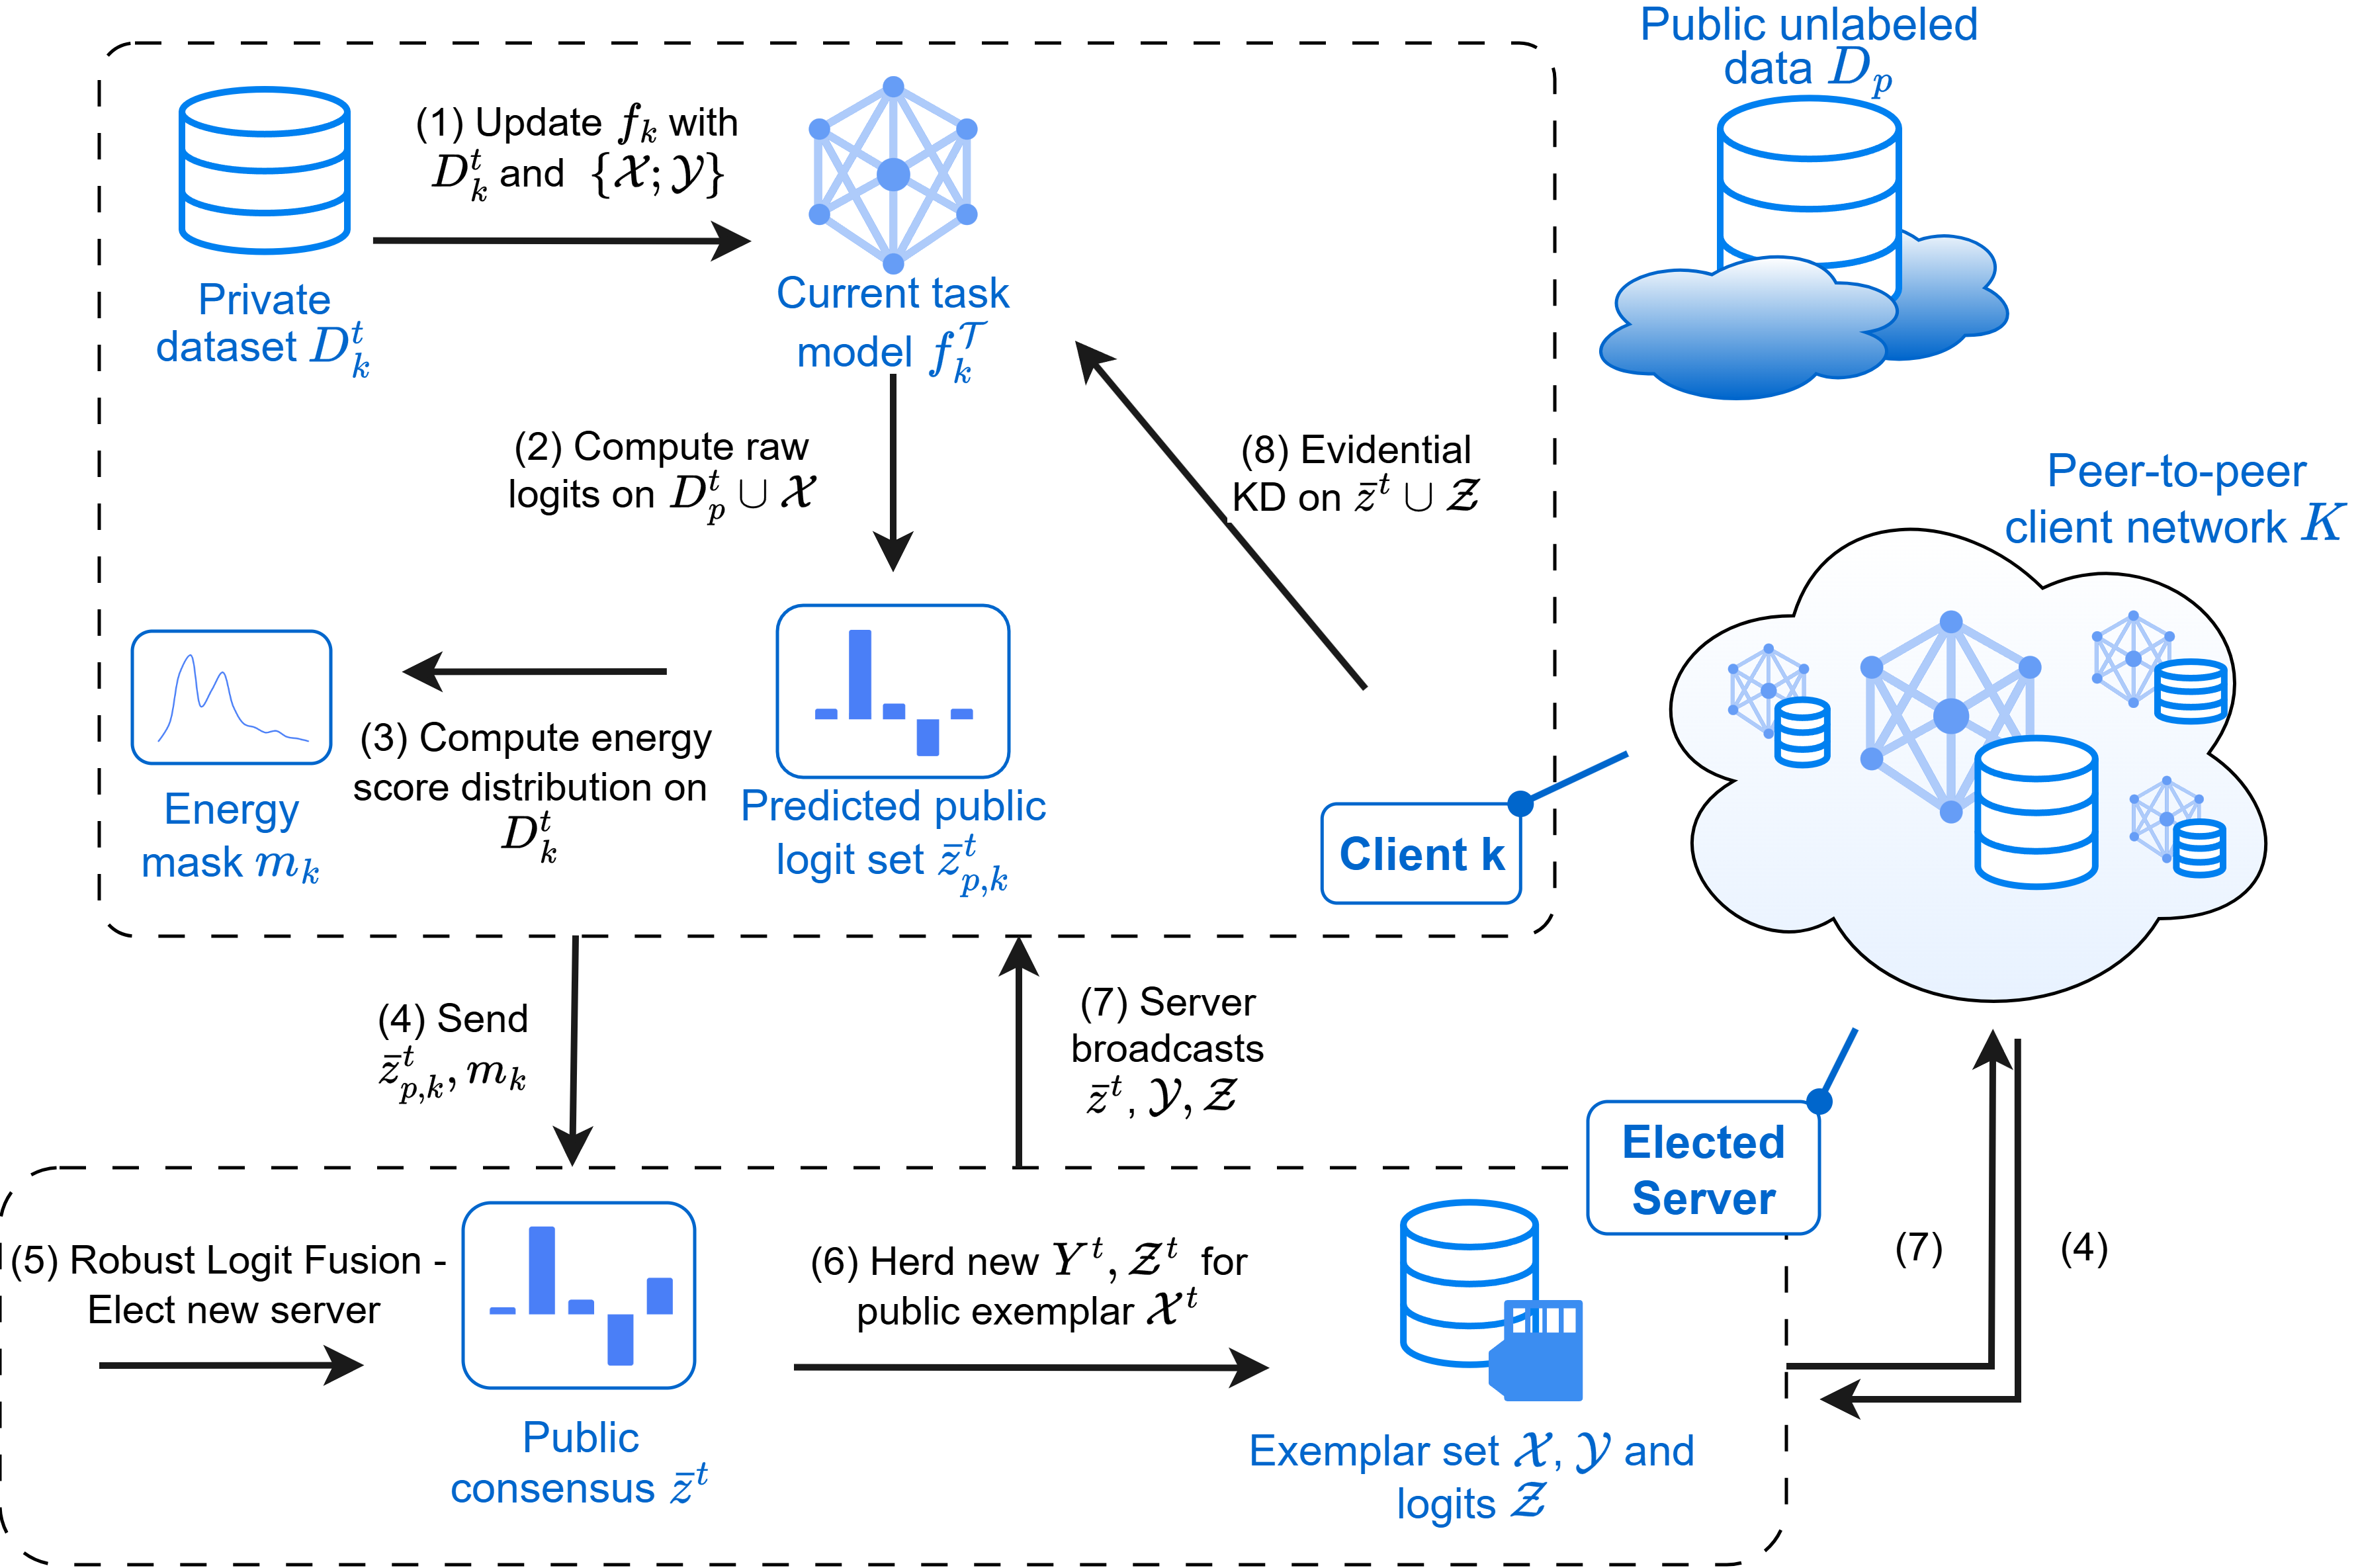
\includegraphics[width=1.0\textwidth]{images/FCIL_ours3.png}
    \caption{Kiến trúc khái quát của phương pháp đề xuất.}
    \label{fig:pipeline}
\end{figure*}

Hình \ref{fig:pipeline} minh họa quy trình hoạt động của hệ thống đề xuất. Thuật toán \ref{alg:proposed_fd_cil_flow} được đặt ngay sau sơ đồ để làm điểm tham chiếu chính; các bước 1--8 trong thuật toán đi theo đúng thứ tự trong hình, và các công thức đi kèm được đánh số để có thể được dẫn chiếu trực tiếp trong phần diễn giải.

\begin{algorithm}[H]
    \LinesNumbered
    \newcommand{\algwrap}[2][1]{\parbox[t]{\dimexpr\linewidth-#1\algomargin-1.5em\relax}{\raggedright#2}}
    \KwInput{\algwrap[3]{Chuỗi task $\{\mathcal{T}_t\}_{t=1}^{T}$, tập client theo task $K_t$, dữ liệu riêng $D_k^t$, tập public $D_p^t$, số vòng $R_t$, quantile energy $q$, ngưỡng robust $\theta$, tỉ lệ nhớ $m$}}
    \KwOutput{\algwrap[3]{Các mô hình cục bộ cuối $\{w_k^T\}$ cùng $\mathcal X^T$, $\mathcal Y^T$, $\mathcal Z^T$}}
    $\mathcal X^0\gets\emptyset$, $\mathcal Y^0\gets\emptyset$, $\mathcal Z^0\gets\emptyset$\;
    Chọn ngẫu nhiên client điều phối đầu tiên từ $K_1$\;
    \For{$t\gets1$ \KwTo $T$}{
        Mở rộng classifier head theo tập lớp mới của $\mathcal{T}_t$\;
        \For{$r\gets1$ \KwTo $R_t$}{
            \ForEach{client $k\in K_t$}{
                \textbf{1.} Cập nhật $f_k$ với $D_k^t$ và $(\mathcal X^{<t},\mathcal Y^{<t})$\;
                \textbf{2.} Tính raw logits $z_{p,k}^t$ trên $D_p^t\cup\mathcal X^{<t}$\;
                \textbf{3.} Tính phân phối energy trên $D_k^t$ và tạo mặt nạ $m_k^t$\;
                \textbf{4.} Gửi $(z_{p,k}^t,m_k^t)$ cho client điều phối\;
            }
            \ForEach{$x\in D_p^t$}{
                \textbf{5.} Robust Logit Fusion trên $\{z_k^t(x)\mid k\in K_t\}$, tính consensus $\bar z^t(x)$ và chọn client điều phối mới\;
            }
            \ForEach{$x\in\mathcal X^{<t}$}{
                Tính consensus replay mới và giữ lại logits hợp lệ trong $\mathcal Z$ nếu nhãn dự đoán khớp $\mathcal Y$\;
            }
            \If{$r=R_t$}{
                \ForEach{pseudo class $c$ từ $\hat y^t(x)=\arg\max_c\bar z_c^t(x)$ trên $D_p^t$}{
                    \textbf{6.} Herd nhãn giả $\mathcal Y^t$, logits $\mathcal Z^t$ và public exemplar $\mathcal X^t$\;
                }
            }
            \textbf{7.} Client điều phối broadcast $\bar z^t$, $\mathcal Y$ và $\mathcal Z$ cho các client\;
            \ForEach{client $k\in K_t$}{
                \textbf{8.} Chắt lọc EKD trên $\bar z^t\cup\mathcal Z$ để cập nhật $f_k$\;
            }
        }
    }
    \Return $\{w_k^T\}$, $\mathcal X^T$, $\mathcal Y^T$, $\mathcal Z^T$\;
    \caption{Luồng hoạt động FD-CIL của phương pháp đề xuất với replay public}
    \label{alg:proposed_fd_cil_flow}
\end{algorithm}

Trước khi đi vào bước 1 của Thuật toán \ref{alg:proposed_fd_cil_flow}, hệ thống xác định tập lớp mới của task hiện tại, tập client tham gia, dữ liệu riêng của từng client và tập public dùng làm bề mặt chung để trao đổi tri thức. Tại task $t$, mỗi client $k\in K_t$ sở hữu dữ liệu riêng $D_k^t$, trong khi toàn hệ thống cùng dùng tập public không gán nhãn $D_p^t$ để trao đổi tri thức ở mức logits. Mô hình cục bộ của client được ký hiệu là $f_k^t$, và logit trước softmax của client $k$ trên mẫu $x$ được ký hiệu là $z_k^t(x)$. Ký hiệu logits được giữ xuyên suốt chương này vì cơ chế EVA, Robust Logit Fusion và EKD đều khai thác độ lớn của logits thay vì dùng xác suất sau softmax.

\subsubsection{Trạng thái dữ liệu và bộ nhớ dữ liệu tái diễn}

Trong học tiệm tiến, nếu client chỉ học dữ liệu của task mới, mô hình dễ dịch chuyển khỏi những lớp đã học ở các task trước (catastrophic forgetting). Tuy nhiên, lưu lại dữ liệu riêng của client cũ không phù hợp với ràng buộc phân tán và quyền riêng tư của hệ thống. Vì vậy, phương pháp đề xuất sử dụng học tiệm tiến dựa trên replay đến từ các mẫu public $x \in D_p$, trong đó những mẫu được giữ lại $\mathcal X$ đều lấy từ tập public $D_p$ thay vì lấy từ dữ liệu riêng. Bộ nhớ replay gồm ba thành phần: $\mathcal X$ lưu các mẫu dữ liệu không nhãn đã chọn để replay, $\mathcal Y$ lưu nhãn cứng tính từ bộ consensus tương ứng, còn $\mathcal Z$ lưu phần logits exemplar hợp lệ dùng làm tín hiệu mềm trong EKD. Trong ba thành phần này, $\mathcal Y$ chỉ được mở rộng ở cuối task, trong khi $\mathcal Z$ được làm mới liên tục ở từng vòng liên kết và kiểm tra lại ở các task sau trước khi tham gia chắt lọc. Bên cạnh đó, các mô hình khi chuyển sang một tác vụ mới cần phải mở rộng đầu ra của lớp phân loại. Đây là một đặc điểm của học tiệm tiến dựa trên dynamic architecture. Thay vì trực tiếp chắt lọc phân phối của mô hình cũ cho mô hình mới, phương pháp đề xuất chắt lọc tri thức chung của các client sau bước học replay cho mô hình mới, kết hợp học liên kết và học tiệm tiến trong cùng một bước chiết xuất.

\subsubsection{Bước 1: Cập nhật mô hình cục bộ bằng dữ liệu hiện tại và tái diễn dữ liệu}

Ở bước 1, client cần cập nhật $f_k$ bằng dữ liệu hiện tại nhưng vẫn được nhắc lại các lớp cũ. Với task đầu tiên, bộ nhớ replay rỗng nên client chỉ tối ưu trên dữ liệu riêng $D_k$ hiện tại. Từ task thứ hai trở đi, đầu ra phân loại của mô hình được mở rộng để cùng chiều với tổng số nhãn (cũ và mới), trong khi dữ liệu huấn luyện cục bộ được tạo bằng cách ghép dữ liệu riêng của task mới với các public exemplars cũ $D_k \cup \mathcal X$ đã có nhãn cứng $\mathcal Y$:
\begin{equation}
\label{eq:local_replay_dataset}
	\tilde D_k^t=D_k^t\cup(\mathcal X^{<t},\mathcal Y^{<t}).
\end{equation}
Với mẫu $(x,y)\in\tilde D_k^t$, client tối ưu hàm mất mát cross-entropy có giám sát:
\begin{equation}
\label{eq:local_ce_loss}
L_{local,k}^t=\frac{1}{|\tilde D_k^t|}\sum_{(x,y)\in\tilde D_k^t}CE(y,p_k^t(x)),
\qquad p_k^t(x)=\operatorname{softmax}(z_k^t(x)).
\end{equation}
Cách ghép trong công thức \ref{eq:local_replay_dataset} đặt quá trình replay ngay trong bước 1, nên CIL không còn là một cơ chế tách rời sau FD. Lớp mới được học từ dữ liệu riêng có nhãn thật, còn lớp cũ được nhắc lại bằng public exemplars đã được consensus gán nhãn ở các task trước thông qua hàm mục tiêu trong công thức \ref{eq:local_ce_loss}. Sau khi cập nhật cục bộ, bước 2 yêu cầu client sinh raw logits $z_{p,k}^t$ trên $D_p^t\cup\mathcal X^{<t}$, nhờ đó task hiện tại và replay features cũ cùng đi vào không gian dự đoán chung trước khi được lọc và tổng hợp.

\subsubsection{Bước 2: Sinh logits cho dữ liệu công khai}

Sau khi đã học giám sát kết hợp học tiệm tiến replay ở bước 1, hệ thống cần cập nhật các mẫu logit replay của các mẫu replay public, vì số chiều của logit đã tăng lên theo số lớp. Như vậy, bên cạnh việc dự đoán logit cho các mẫu public thuộc task hiện $D_p^t$, các mô hình còn cần dự đoán cả các mẫu exemplar $\mathcal X$ trên tập dữ liệu public từ task trước. Sau bước 2, ở mỗi client đã tồn tại tập dự đoán $z \leftarrow \bar z_{p,k}^t \cup \mathcal Z_k$, trong đó $\bar z_{p,k}^t$ là phân phối logit của tập dữ liệu public ở tác vụ $t$ của mô hình thuộc client $k$, cũng như $\mathcal Z_k$ là phân phối logit của dữ liệu replay của tất cả các tác vụ trước do mô hình $f_k$ dự đoán.

\subsubsection{Bước 3: Sinh phân phối energy và chọn ngưỡng lọc trong EVA}

Tập public giúp các client gặp nhau ở cùng một không gian dự đoán, nhưng không phải public sample nào cũng nằm gần phân phối riêng của mọi client. Nếu mọi client đều đóng góp logits với cùng mức tin cậy, consensus có thể bị kéo lệch bởi những dự đoán thiếu cơ sở. Vì vậy, EVA được đưa vào để mỗi client tự đánh giá public sample nào thuộc gần phân phối dữ liệu riêng của mình thành trọng số tổng hợp đi kèm dự đoán để logits được tổng hợp ổn định hơn.

Phát hiện ngoài phân phối bằng energy (Energy-based Out-of-distribution detection) xuất phát từ nhận xét rằng xác suất softmax lớn nhất của mô hình thường quá tự tin ngay cả với mẫu ngoài phân phối, vì softmax không nhạy với phép dịch trên logit \cite{liu2020energy}. Với logit $z_i$ và temperature $T$, energy của mẫu $x$ được định nghĩa là
\begin{equation}
\label{eq:energy_general}
E(x) = -T\log\sum_i e^{z_i/T}.
\end{equation}
Giá trị energy thấp thường đi với mẫu nằm trong phân phối huấn luyện, vì mô hình tạo ra một hoặc nhiều logit có độ lớn đủ cao để kéo giá trị log-sum-exp lên. Ngược lại, giá trị energy cao cho thấy các giá trị logit thường trải đều và thấp, nên các mẫu với energy cao có khả năng thuộc vùng ngoài phân phối. Trong IDS, cách nhìn này hữu ích vì lưu lượng mới, biến thể tấn công mới hoặc mẫu bị nhiễu không nhất thiết tạo ra xác suất softmax thấp, nhưng vẫn có thể biểu hiện qua energy cao hơn so với các mẫu quen thuộc.

Ở bước 3, với logit $z_k^t(x)$, energy của client $k$ được tính bằng
\begin{equation}
\label{eq:client_energy}
E_k^t(x)=-T\log\sum_i\exp(z_{k,i}^t(x)/T).
\end{equation}
Ngưỡng lọc của client được ước lượng từ phân phối energy trên dữ liệu riêng hiện tại:
\begin{equation}
\label{eq:eva_threshold}
\tau_k^t=Q_q(\{E_k^t(x)\mid x\in D_k^t\}).
\end{equation}
Sau đó, client sinh logits trên cả public samples của task hiện tại và replay features cũ, rồi tạo mặt nạ EVA:
\begin{equation}
\label{eq:eva_mask}
m_k^t(x)=\mathbb{I}[E_k^t(x)\leq\tau_k^t],\qquad x\in D_p^t\cup\mathcal X^{<t}.
\end{equation}
Ở bước 4, client gửi cặp $(z_k^t(x),m_k^t(x))$ cho phần tử điều phối. Nhờ mặt nạ trong công thức \ref{eq:eva_mask}, dự đoán có energy cao vẫn có thể được ghi nhận, nhưng không được xem là đóng góp đáng tin trong bước logit fusion.

\subsection{Bước 4: Client cập nhật phân phối logit và mặt nạ EVA lên phần tử điều phối}

Sau khi tất cả các client đã hoàn thành bước 3, ở mỗi client $k \in K^t$ tham gia vòng liên kết đó đã tồn tại bộ logit dự đoán cho tập dữ liệu public $\bar z_{p,k}^t$ và tập replay public $\mathcal Z_k$, cũng như mặt nạ EVA cho cả hai tập logit này $m_k$. Toàn bộ client upload các dữ liệu này về client đảm nhiệm vai trò điều phối để tiến hành tổng hợp.

\subsubsection{Bước 5: Robust Logit Fusion và lựa chọn phần tử điều phối}

EVA làm giảm ảnh hưởng của những dự đoán nằm ngoài phân phối riêng của từng client, nhưng trong tập logits gửi về vẫn có thể tồn tại những vector quá lệch so với phần còn lại do Non-IID, kéo giá trị tổng hợp theo hướng bất lợi. Vì vậy, Blom Robust Filter được dùng như tầng làm sạch thứ hai trước khi tổng hợp consensus sau cùng.

Cụ thể, ở bước 5, với tập client đang hoạt động $K^a$, hệ thống tính trung bình và covariance của các logits, lấy eigenvector cao nhất $v(x)$, rồi ánh xạ từng logit lên hướng này:
\begin{equation}
\label{eq:robust_projection}
s_k^t(x)=v(x)^\top(z_k^t(x)-\bar z^{a,t}(x)),\qquad k\in K^a.
\end{equation}
Median projection và thang đo MAD được tính bằng
\begin{equation}
\label{eq:robust_mad}
\tilde s^t(x)=\operatorname{median}_{k\in K^a}s_k^t(x),
\qquad
\sigma^t(x)=1.4826\cdot\operatorname{median}_{k\in K^a}|s_k^t(x)-\tilde s^t(x)|.
\end{equation}
Độ lệch chuẩn hóa của client là
\begin{equation}
\label{eq:robust_distance}
d_k^t(x)=\frac{|s_k^t(x)-\tilde s^t(x)|}{\sigma^t(x)}.
\end{equation}
Các giá trị này được so sánh với ngưỡng Blom theo rank để tạo mặt nạ outlier $o_k^t(x)$. Sau khi có mặt nạ outlier và mặt nạ EVA, consensus trên public sample hiện tại được tính bằng
\begin{equation}
\label{eq:consensus_logit}
\bar z^t(x)=\frac{\sum_{k\in K_t}m_k^t(x)(1-o_k^t(x))z_k^t(x)}{\sum_{k\in K_t}m_k^t(x)(1-o_k^t(x))},\qquad x\in D_p^t.
\end{equation}
Tỉ lệ bị loại của từng client được tính trên tập public:
\begin{equation}
\label{eq:filter_score}
\rho_k^t=\frac{1}{|D_p^t|}\sum_{x\in D_p^t}o_k^t(x).
\end{equation}
Client có $\rho_k^t$ thấp hơn cho thấy logits của nó ít bị xem là outlier hơn, nên hệ thống chọn phần tử điều phối của vòng tiếp theo từ các client có filter score $\rho_k^t$ thấp nhất ngay trong bước 5. Nhờ vậy, cơ chế điều phối vẫn giữ bản chất phi tập trung nhưng ưu tiên client đang tạo tri thức ổn định hơn.

\subsubsection{Bước 6: Cập nhật dữ liệu tái diễn}

Sau bước 5, mẫu replay từ tập dữ liệu public cũ không chỉ tham gia học giám sát cross-entropy, mà còn tham gia vào giai đoạn chắt lọc ở sau bước tổng hợp. Tuy nhiên, logits mềm cũ không tương thích trực tiếp, vì không gian lớp đã mở rộng sau mỗi task. Do đó, với mỗi mẫu cũ $x\in\mathcal X^{<t}$, client sinh lại logits sử dụng mô hình $f_k$ sau bước học giám sát trên $D_k \cup \{\mathcal X, \mathcal Y\}$ hiện tại. Phần tử điều phối tổng hợp các logit đã cập nhật số chiều này song song với logit của task hiện tại, rồi tạo consensus replay mới $\mathcal Z$ để chuẩn bị cho bước broadcast.

Nếu bước này xảy ra trong vòng liên kết cuối cùng của task, hệ thống cần herd một phần dữ liệu public của tác vụ hiện tại để phục vụ quá trình học tiệm tiến replay các task sau. Việc lưu toàn bộ public là không cần thiết và làm tăng chi phí replay, nên phương pháp đề xuất chỉ giữ những mẫu có consensus logits gần trung tâm của từng pseudo class. Với consensus $\bar z$ trên $D_p^t$, nhãn cứng của public sample được xác định bằng
\begin{equation}
\label{eq:pseudo_label}
\hat y^t(x)=\arg\max_c\bar z_c^t(x).
\end{equation}
Các mẫu được gom theo pseudo class:
\begin{equation}
\label{eq:pseudo_group}
G_c^t=\{x\in D_p^t\mid \hat y^t(x)=c\},
\qquad
\mu_c^t=\frac{1}{|G_c^t|}\sum_{x\in G_c^t}\bar z^t(x).
\end{equation}
Với mỗi lớp giả $c$, hệ thống chọn $m\%$ mẫu có logit gần $\mu_c^t$ nhất:
\begin{equation}
\label{eq:exemplar_select}
\mathcal X_c^t=\operatorname{TopClose}_{m\%}\{x\in G_c^t;\|\bar z^t(x)-\mu_c^t\|_2\}.
\end{equation}
Bộ nhớ replay được mở rộng ở cuối task bằng
\begin{equation}
\label{eq:memory_update_xy}
\mathcal X^t=\mathcal X^{<t}\cup\bigcup_c\mathcal X_c^t,
\qquad
\mathcal Y^t=\mathcal Y^{<t}\cup\bigcup_c\{\hat y^t(x)\mid x\in\mathcal X_c^t\},
\end{equation}
\begin{equation}
\label{eq:memory_update_z}
\mathcal Z^t=\mathcal Z^{<t}\cup\bigcup_c\{\bar z^t(x)\mid x\in\mathcal X_c^t\}.
\end{equation}
$\mathcal Y$ được nối thêm một lần cho task hiện tại, còn $\mathcal Z$ lưu consensus tại thời điểm chọn mẫu nhưng vẫn sẽ được làm mới và kiểm chứng lại khi replay xuất hiện trong task sau.

Bộ logit replay chỉ được chấp nhận nếu nhãn dự đoán của nó vẫn khớp với nhãn $\mathcal Y$:
\begin{equation}
\label{eq:replay_consistency}
\arg\max_c\mathcal Z_c(x)=y_x,\qquad y_x\in\mathcal Y^{<t}.
\end{equation}
Điều này làm rõ vai trò khác nhau của $\mathcal Y$ và $\mathcal Z$. Tập $\mathcal Y$ là tập nhãn cứng không đổi theo thời gian, chỉ được nối thêm ở cuối các task và không bị sửa lại ở các vòng sau. Ngược lại, $\mathcal Z$ được cập nhật liên tục: nó được làm mới từ $\mathcal X$ dưới không gian lớp hiện tại, sau đó bị lọc bằng $\mathcal Y$. Vì vậy, số logits hợp lệ trong $\mathcal Z$ ở một vòng có thể nhỏ hơn số nhãn đang được lưu trong $\mathcal Y$.

\subsubsection{Bước 7: Cập nhật bộ logit tổng hợp và nhãn cứng cho học tái diễn}

Sau khi tổng hợp, phần tử điều phối broadcast bộ dữ liệu replay gồm đặc trưng $\mathcal X$ và logits hợp lệ $\mathcal Z$ cũng như bộ logit của tác vụ hiện tại $\bar z^t$ trên dữ liệu public cho mọi client tham gia. Như đã giải thích ở bước 6, logits replay và logits của tác vụ hiện tại luôn được cập nhật và trả về ở mỗi vòng liên kết, trong khi bộ nhãn cứng replay chỉ được cập nhật và thêm mới ở cuối task $t$. Do đó, phần tử điều phối cũng broadcast kèm bộ nhãn replay $\mathcal Y$ đã cập nhật ở vòng liên kết cuối cùng mỗi task.

\subsubsection{Bước 8: Evidential Knowledge Distillation}

Ở bước 8, sau khi có consensus trên $D_p^t$ và phần replay logits hợp lệ $\mathcal Z$, phần tử điều phối broadcast teacher logits $\bar z^t(x)$, nhãn giả $\mathcal Y$ và logits replay $\mathcal Z$ về các client. Mục tiêu của bước 8 là đưa tri thức đã được tổng hợp quay lại toàn bộ client tham gia, nhưng vẫn không yêu cầu trao đổi trọng số mô hình. Phương pháp đề xuất dùng EKD vì logits không chỉ chứa thứ tự ưu tiên giữa các lớp, mà còn phản ánh mức bằng chứng và độ chắc chắn của consensus.

Với teacher logit $\bar z^t(x)$ và student logit $z_k^t(x)$ từ các mẫu public $x \in D_p$, tham số Dirichlet được tạo bằng
\begin{equation}
\label{eq:dirichlet_evidence}
\alpha^T(x)=\exp(\bar z(x))+\lambda_{prior},
\qquad
\alpha_k^S(x)=\exp(z_k(x))+\lambda_{prior}.
\end{equation}
Mất mát EKD gồm tầng căn chỉnh tỷ lệ bằng chứng và tầng căn chỉnh toàn bộ phân phối Dirichlet:
\begin{equation}
\label{eq:ekd_loss}
L_{EKD,k}^t=L_{1st,k}^t+\gamma L_{2nd,k}^t.
\end{equation}
Bước chắt lọc này tách hẳn khỏi giai đoạn học giám sát trước đó, nên mỗi vòng huấn luyện của client được chia thành hai pha tuần tự thay vì gộp chung vào một hàm mất mát duy nhất. Ở pha thứ nhất, client tối ưu riêng mục tiêu giám sát $L_{local,k}^t$ trên dữ liệu riêng cùng nhãn cứng trong quá trình replay, qua đó học các lớp mới và củng cố tri thức cũ:
\begin{equation}
\label{eq:local_update}
\theta_k^{t,\,\text{(1)}}\leftarrow\arg\min_{\theta_k}L_{local,k}^t.
\end{equation}
Sau bước 7, khi đã có được bộ logit từ nhãn công khai hiện tại và replay, từng client tối ưu mục tiêu chắt lọc $L_{EKD,k}^t$ trên kiến thức chắt lọc từ mô hình teacher $\bar z$ tại $D_p^t \cup \mathcal X$:
\begin{equation}
\label{eq:ekd_update}
\theta_k^{t,\,\text{(2)}}\leftarrow\arg\min_{\theta_k}L_{EKD,k}^t.
\end{equation}

\subsection{Mô hình phát hiện xâm nhập}

\subsubsection{Đơn mô hình}

Trong thiết lập đơn mô hình, toàn bộ client sử dụng cùng một kiến trúc phát hiện xâm nhập, cùng số chiều đầu ra và cùng cách biểu diễn tham số. Thiết lập này phù hợp với các phương pháp FL dựa trên tổng hợp trọng số vì mô hình của mọi client có cùng cấu trúc, nên server hoặc phần tử điều phối có thể cộng trung bình tham số theo từng lớp. Tuy nhiên, ràng buộc đồng nhất kiến trúc làm giảm tính linh hoạt của hệ thống khi các client có tài nguyên tính toán, kiểu lưu lượng mạng hoặc yêu cầu triển khai khác nhau.

\subsubsection{Đa mô hình}

Trong thiết lập đa mô hình, các client có thể sử dụng các kiến trúc phát hiện xâm nhập khác nhau, chẳng hạn mô hình tuần tự, mô hình tích chập hoặc mô hình lai, miễn là chúng cùng ánh xạ dữ liệu đầu vào về không gian nhãn chung của bài toán. Phương pháp đề xuất hoàn toàn tương thích với thiết lập này vì quá trình cộng tác diễn ra trên logits thay vì trên trọng số mô hình. Mặt khác, energy sinh ra trong bước EVA hoàn toàn phụ thuộc vào từng kiến trúc và phân phối dữ liệu riêng của client, và Robust Logit Fusion cũng như EKD trong Thuật toán \ref{alg:proposed_fd_cil_flow} chỉ yêu cầu các client sử dụng chung số chiều của lớp dự đoán đầu ra (logit layer), một điều kiện hoàn toàn bình thường trong học liên kết.

\section{Đầu ra của hệ thống}

Hệ thống tạo log huấn luyện, file kết quả theo vòng, bản ghi trọng số của mô hình toàn cục hoặc trọng số client theo vòng và các bảng đánh giá cuối. Các đầu ra này phục vụ phân tích hiệu năng, so sánh thuật toán và tái đánh giá.

\chapter{HIỆN THỰC, ĐÁNH GIÁ VÀ THẢO LUẬN}\label{Chapter4}

\section*{Tóm tắt chương}

Chương này trình bày kế hoạch hiện thực và đánh giá hệ thống đề xuất. Nội dung bao gồm môi trường thí nghiệm, chuẩn bị dữ liệu, cấu hình chạy, chỉ số đánh giá, nhóm thí nghiệm và hướng thảo luận kết quả.

\section{Môi trường thực nghiệm}

\begin{itemize}
    \item \textbf{Máy 1}
    \begin{itemize}
        \item CPU: Intel\textregistered{} Core\texttrademark{} i9-13900k (16 cores - 2.9 GHz)
        \item GPU: NVIDIA GeForce\texttrademark{} RTX 3080 10GB LHR
        \item RAM: 22GB
        \item OS: Windows Subsystem for Linux 2 - Debian GNU/Linux 12
        \item Dung lượng ổ đĩa: 1TB
    \end{itemize}
    
    \item \textbf{Máy 2}
    \begin{itemize}
        \item CPU: AMD\textregistered{} Ryzen\texttrademark{} 9-5950X (16 cores - 3.4 Ghz)
        \item GPU: NVIDIA GeForce\texttrademark{} RTX 3090 24GB
        \item RAM: 32GB
        \item OS: Ubuntu GNU/Linux 20.04
        \item Dung lượng ổ đĩa: 870GB
    \end{itemize}

    \item \textbf{Môi trường phát triển}
    \begin{itemize}
        \item Trình soạn thảo: Visual Studio Code, OpenCode.
        \item Ngôn ngữ lập trình: Python3, Bash.
        \item Thư viện sử dụng: numpy, pandas, mathplotlib, sklearn, torch 2.12.0, pickle, cuda 13.2
    \end{itemize}
\end{itemize}

\section{Dữ liệu thực nghiệm}

Bộ dữ liệu được sử dụng trong nghiên cứu này là CICIoT2023 \cite{ciciot2023}, một tập dữ liệu phát hiện xâm nhập quy mô lớn được thu thập trên hạ tầng thiết bị IoT thực tế, trong đó lưu lượng bình thường được ghi nhận song song với nhiều họ tấn công khác nhau nhằm phản ánh sát thực tế vận hành của một hệ thống IDS. Trước khi đưa vào huấn luyện, dữ liệu thô được làm sạch qua bước tiền xử lý, trong đó các bản ghi mang giá trị rỗng, giá trị vô cực hoặc bản ghi trùng lặp đều được loại bỏ, đồng thời các đặc trưng số được chuẩn hoá về cùng một thang đo để tránh việc một vài đặc trưng có biên độ lớn lấn át quá trình học. Sau bước chuẩn hoá, mỗi luồng mạng được biểu diễn bằng một vector đặc trưng $20$ chiều, trong đó $20$ cột đầu đóng vai trò là đầu vào của mô hình còn cột cuối cùng lưu nhãn lớp tương ứng.

Tập đặc trưng $20$ chiều bao quát nhiều khía cạnh của một luồng mạng, từ đặc tính thời gian, kích thước và thống kê gói, đến các cờ giao thức TCP cùng tỉ lệ phân bố giao thức. Bảng \ref{tab:cic23_features} liệt kê đầy đủ $20$ đặc trưng, được nhóm lại theo bản chất nhằm thuận tiện cho phần thảo luận sau này. Việc giới hạn ở $20$ đặc trưng giúp giảm chi phí huấn luyện trong mô phỏng nhiều client, đồng thời vẫn bảo toàn các tín hiệu quan trọng để phân biệt lưu lượng bình thường với các nhóm tấn công, vốn thường khác nhau ở mặt kích thước gói, tần suất truyền và phân bố cờ TCP.

\begin{table}[H]
    \centering
    \caption{Tập $20$ đặc trưng đầu vào của CICIoT2023.}
    \label{tab:cic23_features}
    \begin{tabular}{lp{0.62\linewidth}}
        \hline
        Nhóm đặc trưng & Tên đặc trưng \\
        \hline
        Thời gian luồng       & flow\_duration, IAT \\
        Kích thước gói        & Tot size, Tot sum, AVG, Min, Max, Magnitue, Header\_Length \\
        Cờ TCP (xuất hiện)    & syn\_flag\_number, ack\_flag\_number, psh\_flag\_number, rst\_flag\_number, fin\_flag\_number \\
        Số đếm cờ TCP            & syn\_count, ack\_count, rst\_count \\
        Tỉ lệ giao thức       & TCP, UDP, ICMP \\
        \hline
    \end{tabular}
\end{table}

Tập dữ liệu sau tiền xử lý chứa $46{,}905{,}384$ bản ghi trải trên $34$ lớp, gồm một lớp lưu lượng bình thường (BenignTraffic) và $33$ lớp tấn công thuộc nhiều nhóm khác nhau. Các lớp tấn công này được tổ chức thành những nhóm lớn, bao gồm nhóm tấn công từ chối dịch vụ phân tán (DDoS) với nhiều biến thể như DDoS-ICMP\_Flood, DDoS-SYN\_Flood hay DDoS-UDP\_Flood, nhóm tấn công từ chối dịch vụ (DoS), họ mã độc Mirai, nhóm trinh sát (Recon), nhóm giả mạo như DNS\_Spoofing và MITM-ArpSpoofing, nhóm tấn công tầng web như XSS, SqlInjection và CommandInjection, cùng nhóm dò mật khẩu DictionaryBruteForce.

Một đặc điểm nổi bật của CICIoT2023 là phân phối lớp mất cân bằng nghiêm trọng, điều vốn phản ánh đúng bản chất của dữ liệu an ninh mạng, nơi một số kiểu tấn công xuất hiện với tần suất rất cao trong khi nhiều kiểu khác lại hiếm gặp. Bảng \ref{tab:cic23_dist} liệt kê toàn bộ $34$ lớp cùng số mẫu và tỉ lệ tương ứng trên toàn tập dữ liệu, được sắp xếp theo thứ tự giảm dần của số mẫu. Lớp đa số DDoS-ICMP\_Flood chiếm tới $15.42\%$ tổng số bản ghi, gấp khoảng $5{,}750$ lần so với lớp Uploading\_Attack vốn chỉ có $1{,}257$ mẫu. Mười lớp giàu mẫu nhất, đều thuộc nhóm DDoS hoặc DoS, đã chiếm hơn $90\%$ toàn tập, trong khi $24$ lớp còn lại chia nhau chưa tới $10\%$. Sự chênh lệch hàng nghìn lần giữa lớp giàu nhất và lớp nghèo nhất khiến cho việc phát hiện các lớp thiểu số trở thành thách thức trọng tâm, đặc biệt khi dữ liệu lại tiếp tục bị phân mảnh và lệch nhãn trong môi trường học liên kết.

\begin{table}[H]
    \centering
    \caption{Phân phối toàn bộ $34$ lớp trong CICIoT2023, sắp xếp giảm dần theo số mẫu.}
    \label{tab:cic23_dist}
    \small
    \begin{tabular}{rlrr}
        \hline
        ID & Lớp & Số mẫu & \% \\
        \hline
        6  & DDoS-ICMP\_Flood          & 7{,}234{,}033 & 15.42 \\
        4  & DDoS-UDP\_Flood           & 5{,}437{,}630 & 11.59 \\
        5  & DDoS-TCP\_Flood           & 4{,}518{,}631 & 9.63 \\
        2  & DDoS-PSHACK\_Flood        & 4{,}114{,}128 & 8.77 \\
        3  & DDoS-SYN\_Flood           & 4{,}078{,}425 & 8.70 \\
        1  & DDoS-RSTFINFlood          & 4{,}064{,}317 & 8.66 \\
        7  & DDoS-SynonymousIP\_Flood  & 3{,}614{,}936 & 7.71 \\
        13 & DoS-UDP\_Flood            & 3{,}334{,}095 & 7.11 \\
        15 & DoS-TCP\_Flood            & 2{,}683{,}771 & 5.72 \\
        14 & DoS-SYN\_Flood            & 2{,}038{,}148 & 4.35 \\
        0  & BenignTraffic             & 1{,}103{,}395 & 2.35 \\
        17 & Mirai-greeth\_flood       & 996{,}594     & 2.12 \\
        19 & Mirai-udpplain            & 894{,}884     & 1.91 \\
        18 & Mirai-greip\_flood        & 755{,}288     & 1.61 \\
        10 & DDoS-ICMP\_Fragmentation  & 454{,}621     & 0.97 \\
        26 & MITM-ArpSpoofing          & 309{,}025     & 0.66 \\
        9  & DDoS-UDP\_Fragmentation   & 288{,}317     & 0.61 \\
        8  & DDoS-ACK\_Fragmentation   & 286{,}488     & 0.61 \\
        25 & DNS\_Spoofing             & 179{,}738     & 0.38 \\
        24 & Recon-HostDiscovery       & 135{,}030     & 0.29 \\
        21 & Recon-OSScan              & 98{,}684      & 0.21 \\
        22 & Recon-PortScan            & 82{,}683      & 0.18 \\
        16 & DoS-HTTP\_Flood           & 72{,}211      & 0.15 \\
        23 & VulnerabilityScan         & 37{,}525      & 0.08 \\
        12 & DDoS-HTTP\_Flood          & 28{,}917      & 0.06 \\
        11 & DDoS-SlowLoris            & 23{,}526      & 0.05 \\
        33 & DictionaryBruteForce      & 13{,}121      & 0.03 \\
        27 & BrowserHijacking          & 5{,}889       & 0.01 \\
        32 & CommandInjection          & 5{,}435       & 0.01 \\
        31 & SqlInjection              & 5{,}272       & 0.01 \\
        29 & XSS                       & 3{,}862       & 0.01 \\
        28 & Backdoor\_Malware         & 3{,}236       & 0.01 \\
        20 & Recon-PingSweep           & 2{,}272       & 0.00 \\
        30 & Uploading\_Attack         & 1{,}257       & 0.00 \\
        \hline
    \end{tabular}
\end{table}

Toàn bộ tập dữ liệu sau tiền xử lý được phân hoạch cho client theo ngữ cảnh Non-IID, đồng thời một tập kiểm thử toàn cục được giữ cố định và dùng chung cho mọi thuật toán nhằm bảo đảm việc so sánh diễn ra trên cùng một thước đo. Tập kiểm thử này được tách theo phân tầng giữ nguyên tỉ lệ lớp, nên phân phối nhãn trên tập kiểm thử trùng khớp với phân phối trên toàn tập, qua đó các lớp thiểu số vẫn hiện diện đầy đủ trong quá trình đánh giá.

Sau khi dữ liệu được tách theo lớp, mỗi lớp được phân bổ cho client theo ngữ cảnh Non-IID lệch nhãn (label skew), trong đó số mẫu của một lớp trên các client được lấy từ phân phối Dirichlet:
\[
\pi_c\sim \operatorname{Dir}(\alpha\mathbf{1}_{|K|}),
\qquad
n_{k,c}=\left\lfloor \pi_{k,c}N_c\right\rfloor,
\]
trong đó $N_c$ là số mẫu của lớp $c$, $|K|$ là số client và $n_{k,c}$ là số mẫu lớp $c$ được cấp cho client $k$. Vì phép lấy mẫu được lặp lại độc lập cho từng lớp, một client có thể giàu dữ liệu ở vài lớp nhưng thiếu nghiêm trọng ở các lớp khác, phản ánh tình huống IDS trong đó mỗi tổ chức chỉ quan sát một phần của không gian tấn công. Tham số $\alpha$ điều khiển mức độ lệch nhãn, và giá trị cụ thể được lựa chọn cho từng kịch bản thực nghiệm sẽ được trình bày ở phần sau. Phân phối thu được khi $\alpha=0.1$ được minh họa trong hình \ref{fig:partition}.

\section{Kịch bản thực nghiệm}

Nghiên cứu này được tiến hành nhằm đánh giá và so sánh năng lực của các phương pháp học tiệm tiến theo lớp khi vận hành trong điều kiện hệ thống phát hiện xâm nhập phải liên tục mở rộng theo thời gian. Quá trình thực nghiệm đặt phương pháp đề xuất bên cạnh một tập rộng các phương pháp học tiệm tiến tiêu biểu, được phân thành ba nhóm chính, bao gồm nhóm dựa trên ràng buộc tham số (EWC, MAS, LwF, PASS, CBKD EFCIL), nhóm dựa trên học tái diễn (iCaRL, BiC) và nhóm dựa trên kiến trúc động (FOSTER); ngoài ra, một cấu hình học liên kết không có cơ chế tiệm tiến (fine tuning) cũng được giữ lại làm cận dưới để làm nổi bật mức độ quên thảm khốc khi không áp dụng bất kỳ biện pháp giữ tri thức nào. Mục tiêu chính của quá trình so sánh là làm rõ khả năng của từng phương pháp trong việc tiếp nhận các lớp tấn công mới mà vẫn duy trì tri thức đã học, đồng thời quan sát chi phí truyền thông mà mỗi phương pháp phải gánh chịu trong từng vòng trao đổi.

Để phản ánh sát thực tế triển khai, toàn bộ hệ thống được thiết kế với $100$ client, trong đó dữ liệu của các client được chia thành $7$ task học tiệm tiến nối tiếp nhau. Mỗi task trong quá trình huấn luyện được gắn với một nhóm lớp tấn công mới hoàn toàn chưa từng xuất hiện ở các task trước, đồng thời cũng đi kèm một nhóm client mới gia nhập hệ thống. Cách tổ chức này được lựa chọn nhằm mô phỏng tình huống trong đó mạng lưới IDS liên kết được mở rộng dần qua thời gian, vừa do số lượng tổ chức tham gia tăng lên, vừa do không gian tấn công mà hệ thống phải nhận diện ngày càng phong phú. Trong mọi task, dữ liệu của nhóm client đang hoạt động được phân hoạch lại theo phân phối Dirichlet với tham số $\alpha=0.1$, qua đó tái tạo ngữ cảnh Non-IID lệch nhãn nghiêm trọng, nơi mỗi client chỉ quan sát được một phần nhỏ của không gian tấn công.

Số lượng client tham gia được thiết kế tăng dần theo từng task nhằm mô phỏng quá trình các tổ chức mới lần lượt gia nhập hệ thống IDS liên kết. Ở task đầu tiên, chỉ có $40$ client tham gia huấn luyện; sau đó, mỗi task tiếp theo bổ sung thêm $10$ client, cho đến khi task cuối cùng quy tụ toàn bộ $100$ client của hệ thống. Bảng \ref{tab:cil_client_growth} tóm tắt số lượng client tích luỹ cùng số client mới gia nhập ở từng task, qua đó cho thấy quá trình mở rộng quy mô của hệ thống diễn ra đều đặn theo thời gian.

\begin{table}[H]
    \centering
    \caption{Số lượng client theo từng task trong kịch bản học tiệm tiến.}
    \label{tab:cil_client_growth}
    \begin{tabular}{cccc}
        \hline
        Task & Client tích luỹ & Client mới & Tỉ lệ (\%) \\
        \hline
        0 & 40  & 40 & 40\% \\
        1 & 50  & 10 & 50\% \\
        2 & 60  & 10 & 60\% \\
        3 & 70  & 10 & 70\% \\
        4 & 80  & 10 & 80\% \\
        5 & 90  & 10 & 90\% \\
        6 & 100 & 10 & 100\% \\
        \hline
    \end{tabular}
\end{table}

Song song với quá trình mở rộng số lượng client, không gian lớp tấn công mà hệ thống phải xử lý cũng được mở rộng theo từng task. Toàn bộ $34$ lớp của tập dữ liệu được phân bổ vào bảy task, trong đó sáu task đầu mỗi task tiếp nhận $5$ lớp mới, còn task cuối cùng tiếp nhận $4$ lớp còn lại. Bảng \ref{tab:cil_task_classes} trình bày chi tiết phân bổ lớp theo từng task, cho thấy mỗi task đều đưa vào hệ thống một tập lớp hoàn toàn mới mà các phương pháp học tiệm tiến phải tiếp nhận mà không được quên tri thức đã tích luỹ từ những task trước. Lớp Benign được cố định ở task đầu tiên, trong khi các lớp tấn công còn lại hoàn toàn được chọn ngẫu nhiên cho từng task.

\begin{table}[H]
    \centering
    \caption{Phân bổ lớp theo từng task trong kịch bản học tiệm tiến.}
    \label{tab:cil_task_classes}
    \small
    \begin{tabular}{clc}
        \hline
        Task & Các lớp trong task & Số lớp \\
        \hline
        0 & BenignTraffic, DictionaryBruteForce, DoS-HTTP\_Flood, & 5 \\
          & BrowserHijacking, Mirai-greip\_flood & \\
        1 & DDoS-UDP\_Fragmentation, DDoS-ICMP\_Fragmentation, & 5 \\
          & Recon-PingSweep, Recon-PortScan, DoS-UDP\_Flood & \\
        2 & DDoS-RSTFINFlood, DDoS-TCP\_Flood, Mirai-greeth\_flood, & 5 \\
          & DDoS-ICMP\_Flood, DoS-SYN\_Flood & \\
        3 & DDoS-HTTP\_Flood, DNS\_Spoofing, DDoS-PSHACK\_Flood, & 5 \\
          & DDoS-SYN\_Flood, Uploading\_Attack & \\
        4 & DDoS-UDP\_Flood, Backdoor\_Malware, Recon-HostDiscovery, & 5 \\
          & SqlInjection, VulnerabilityScan & \\
        5 & Mirai-udpplain, MITM-ArpSpoofing, DDoS-SynonymousIP\_Flood, & 5 \\
          & Recon-OSScan, DictionaryBruteForce & \\
        6 & DDoS-ACK\_Fragmentation, DDoS-SlowLoris, DoS-TCP\_Flood, XSS & 4 \\
        \hline
        \multicolumn{2}{l}{Tổng cộng} & 34 \\
        \hline
    \end{tabular}
\end{table}

Để bảo đảm mỗi client nhận đủ dữ liệu huấn luyện, dữ liệu của từng task được phân hoạch lại hoàn toàn từ đầu chỉ cho nhóm client đang tích cực tham gia task đó. Cách tiếp cận này khác với kịch bản học liên kết thông thường, nơi toàn bộ $100$ client nhận phân hoạch cố định từ đầu; thay vào đó, phân hoạch được tái tạo cho từng task dựa trên số client tham gia lúc đó, qua đó phản ánh đúng tình huống mở rộng mạng lưới liên kết theo thời gian. Sau khi phân hoạch, một tỉ lệ ngẫu nhiên trong khoảng $[5\%, 20\%]$ số mẫu của từng client được tách ra làm phần dữ liệu công khai, phần còn lại giữ làm dữ liệu riêng. Vì tỉ lệ cắt được lấy độc lập cho mỗi client, tổng phần công khai trên toàn hệ thống là $7{,}935{,}448$ mẫu ($16.92\%$), còn $38{,}969{,}936$ mẫu ($83.08\%$) được giữ làm dữ liệu riêng cho huấn luyện giám sát cục bộ.

\begin{figure*}[ht]
    \centering
    
\includegraphics[width=1.0\textwidth]{images/partition.png}
    \caption{Phân phối dữ liệu theo lớp cho 100 client.}
\label{fig:partition}
\end{figure*}

Bên cạnh kịch bản chuẩn trong đó mọi client cùng dùng một loại kiến trúc, đề tài này còn xây dựng thêm một kịch bản mô hình hỗn hợp (mixed model architectures, kí hiệu multiple) nhằm kiểm chứng tính linh hoạt của kỹ thuật học chắt lọc liên kết trong phương pháp đề xuất. Trong kịch bản hỗn hợp, các client trong hệ thống được phép sử dụng những kiến trúc mạng khác nhau thay vì bị ràng buộc chung một mô hình, qua đó phản ánh tình huống thực tế nơi mỗi tổ chức tự lựa chọn cấu hình phù hợp với hạ tầng riêng. Quá trình trao đổi tri thức giữa các client lúc này không còn dựa trên việc tổng hợp trọng số, mà chuyển sang trao đổi logits trên tập dữ liệu công khai, nhờ đó hệ thống vẫn có thể phối hợp học tập dù mỗi client mang một mô hình khác biệt về cấu trúc.

% Trước khi đi vào kết quả, chi phí truyền thông của từng phương pháp cũng được ước lượng ở mức một client trong một vòng huấn luyện, với giả định mọi tensor số thực dùng định dạng float32 và nhãn cứng dùng int64. Theo hiện thực trong mã nguồn, FedAvg truyền trọng số mô hình cùng một số vô hướng biểu diễn kích thước dữ liệu client; GLFC giữ cơ chế FedAvg nhưng bổ sung các gradient của encoder dùng cho proxy server; FEAT thay tầng phân loại cuối bằng ETF cố định nên không cần truyền trọng số của tầng logits, đồng thời chỉ gửi thêm hai đại lượng năng lượng head--tail; còn phương pháp đề xuất truyền logits trên tập công khai, mặt nạ nhị phân tương ứng và nhận lại logits đồng thuận cùng nhãn giả cứng. Với $C=34$, mô hình có khoảng $259{,}810$ tham số, phần mô hình không tính tầng ETF của FEAT có khoảng $257{,}600$ tham số, encoder của GLFC có khoảng $32{,}258$ tham số, và số mẫu công khai trung bình mỗi task được xấp xỉ bởi $P=7{,}935{,}448/7\approx1.13$ triệu mẫu.

% \begin{table}[H]
%     \centering
%     \caption{Ước lượng chi phí truyền thông mỗi client trong một vòng huấn luyện.}
%     \label{tab:comm_cost_cil}
%     \resizebox{\linewidth}{!}{
%     \begin{tabular}{lcccccc}
%         \hline
%         \multirow{2}{*}{Phương pháp} & \multicolumn{2}{c}{Lý thuyết} & \multicolumn{2}{c}{Thực tế} & \multirow{2}{*}{Tổng} \\
%         \cline{2-5}
%         & Upload & Download & Upload & Download & \\
%         \hline
%         FedAvg & $|\theta|+1$ & $|\theta|$ & $1.04$ MB & $1.04$ MB & $2.08$ MB \\
%         GLFC & $|\theta|+1+G_{\mathrm{enc}}$ & $|\theta|$ & $3.50$ MB & $1.16$ MB & $4.66$ MB \\
%         FEAT & $|\theta|-|\theta_{\mathrm{logits}}|+2$ & $|\theta|-|\theta_{\mathrm{logits}}|$ & $1.03$ MB & $1.03$ MB & $2.06$ MB \\
%         Đề xuất & $(P+E)C$ logits $+(P+E)C$ mask & $(P+E)C$ logits $+(P+E)$ nhãn & $200$ MB & $155.96$ MB & $355.96$ MB \\
%         \hline
%     \end{tabular}}
% \end{table}

% Trong bảng \ref{tab:comm_cost_cil}, $G_{\mathrm{enc}}$ được tính theo giới hạn tối đa $20$ bộ gradient encoder mà GLFC lưu trong \texttt{proto\_grad\_pool}, nên phần phụ trội xấp xỉ $20\times32{,}258\times4=2.58$ MB. Với phương pháp đề xuất, $E$ biểu diễn số mẫu replay từ các task cũ; do cấu hình mặc định giữ khoảng $1\%$ mẫu công khai theo từng lớp, phần này nhỏ hơn nhiều so với $P$ và được gộp vào ước lượng cuối. Vì vậy, phương pháp đề xuất có chi phí lớn hơn ở từng vòng trao đổi, nhưng phần truyền thông này là logits trên dữ liệu công khai và exemplar thay vì trọng số mô hình riêng của client.

\section{Thiết lập thực nghiệm}

\subsection{Cấu hình huấn luyện chung}

Các mô hình chính trong thí nghiệm được hiện thực bằng PyTorch. Đầu vào của mỗi mô hình là vector đặc trưng $x\in\mathbb{R}^{20}$, còn đầu ra là vector logits có kích thước bằng số lớp hiện tại. Trong chế độ dự đoán, logits được đưa qua hàm softmax để tạo phân phối xác suất; trong huấn luyện, loss được tính trực tiếp trên logits để giữ ổn định số học.

Tất cả các mô hình phân loại dùng Adam làm bộ tối ưu. Learning rate mặc định được co giãn theo batch size:
\[
\eta=10^{-3}\sqrt{\frac{B}{1024}},
\]
trong đó $B$ là batch size. Batch size mặc định là $8192$. Learning rate dùng warm-up tuyến tính:
\[
\eta_e= \eta\frac{e+1}{5}
\]
Hàm mất mát cho học giám sát là cross-entropy với label smoothing $0.05$. Gradient được chuẩn hoá bằng clipping theo chuẩn $\ell_2$ với ngưỡng $0.5$. Một số lớp tuyến tính được áp dụng weight decay $10^{-4}$ để giảm overfitting, trong khi các tham số còn lại không dùng weight decay. Các mô hình dùng LayerNorm thay cho BatchNorm vì thí nghiệm có batch lớn, dữ liệu Non-IID và phân phối giữa client khác nhau; LayerNorm giúp chuẩn hoá biểu diễn theo từng mẫu và ít phụ thuộc thống kê batch hơn.

\subsection{Mô hình GRU}
\label{sec:gru_arch}

GRU \cite{kasongo2023gru} xử lý vector 20 chiều như chuỗi một chiều có độ dài 20, mỗi bước thời gian chứa một giá trị đặc trưng. Cách biểu diễn này cho phép mô hình học quan hệ tuần tự tương đối giữa các đặc trưng sau tiền xử lý, đồng thời vẫn giữ chi phí thấp hơn BiLSTM. Bảng \ref{tab:gru_arch} trình bày kiến trúc GRU.

\begin{table}[H]
\centering
\caption{Kiến trúc GRU dùng trong thí nghiệm.}
\label{tab:gru_arch}
\begin{tabular}{lll}
\hline
Tầng & Kích thước & Thiết lập \\
\hline
Reshape & $20\rightarrow20\times1$ & Mỗi đặc trưng là một bước chuỗi \\
GRU 1 & $1\rightarrow128$ & Trả về toàn bộ chuỗi, LayerNorm, Dropout $0.15$ \\
GRU 2 & $128\rightarrow128$ & Trả về toàn bộ chuỗi, LayerNorm, Dropout $0.15$ \\
GRU 3 & $128\rightarrow128$ & Lấy trạng thái cuối, LayerNorm, Dropout $0.15$ \\
Dense head & $128\rightarrow64$ & ReLU, LayerNorm, Dropout $0.20$ \\
Classifier & $64\rightarrow C$ & Logits theo số lớp $C$ \\
\hline
\end{tabular}
\end{table}

Ba tầng GRU liên tiếp cho phép mô hình tích luỹ tương tác phi tuyến giữa các đặc trưng. Hai tầng đầu giữ toàn bộ chuỗi để tầng sau tiếp tục xử lý thông tin theo vị trí đặc trưng, còn tầng cuối chỉ lấy trạng thái cuối làm biểu diễn toàn cục. Dense head dùng ReLU vì đây là tầng nén cuối trước logits, cần ánh xạ rõ ràng và gọn hơn thay vì giữ dạng kích hoạt trơn như MLP. Weight decay chỉ áp dụng lên tầng head, còn các tầng GRU không dùng weight decay để tránh làm yếu khả năng ghi nhớ trong các cổng cập nhật.

Mô hình GRU được sử dụng cho kịch bản đơn kiến trúc để so sánh với các kịch bản học tiệm tiến dựa trên thuật toán FedAvg.

\subsection{Mô hình DCNN--BiLSTM}
\label{sec:dcblstm_arch}
DCNN--BiLSTM \cite{hnamte2023dcnnbilstm} là mô hình sâu hơn, kết hợp trích xuất mẫu cục bộ bằng tích chập một chiều và mô hình hoá phụ thuộc hai chiều bằng BiLSTM. Bảng \ref{tab:dcblstm_arch} mô tả kiến trúc của mô hình này.

\begin{table}[H]
\centering
\caption{Kiến trúc CNN--BiLSTM dùng trong thí nghiệm.}
\label{tab:dcblstm_arch}
\begin{tabular}{lll}
\hline
Tầng & Kích thước & Thiết lập \\
\hline
Reshape & $20\rightarrow1\times20$ & Một kênh đầu vào \\
Conv1D & $1\rightarrow64$ & Kernel size $20$, padding same, ReLU, LayerNorm \\
BiLSTM 1 & $64\rightarrow2\times64$ & Trả về toàn bộ chuỗi, LayerNorm \\
BiLSTM 2 & $128\rightarrow2\times128$ & Lấy trạng thái cuối hai chiều, Dropout $0.10$ \\
DNN 1 & $256\rightarrow64$ & ReLU, Dropout $0.10$ \\
DNN 2 & $64\rightarrow32$ & ReLU, Dropout $0.10$ \\
DNN 3 & $32\rightarrow16$ & ReLU, Dropout $0.10$ \\
LayerNorm & $16$ & Chuẩn hoá biểu diễn cuối \\
Classifier & $16\rightarrow C$ & Logits theo số lớp $C$ \\
\hline
\end{tabular}
\end{table}

Tầng CNN đầu tiên đóng vai trò bộ trích xuất mẫu cục bộ trên toàn bộ vector đặc trưng. Do kernel size bằng số chiều đầu vào, mỗi filter học một phép chiếu có cấu trúc qua toàn bộ đặc trưng, sau đó BiLSTM khai thác biểu diễn theo hai hướng. BiLSTM phù hợp với IDS vì một số đặc trưng lưu lượng có quan hệ phụ thuộc lẫn nhau, ví dụ số gói, kích thước gói và tốc độ truyền. Việc dùng hai tầng BiLSTM giúp mô hình học cả quan hệ thấp và quan hệ trừu tượng hơn, còn khối DNN cuối giảm chiều biểu diễn từ $256$ xuống $64$ trước khi phân loại, và lớp DNN cuối cùng chiều với mô hình GRU (\ref{sec:gru_arch}) để cho phép học liên kết qua chắt lọc prototype (FedProto). Mô hình này không áp dụng weight decay riêng cho các tầng trong cấu hình hiện tại, nhưng vẫn dùng Adam, label smoothing, learning-rate scheduler và gradient clipping giống cấu hình chung.

\subsection{Mô hình Multi Layer Perceptron}

MLP được dùng làm mô hình đơn giản cho dữ liệu vector 20 chiều. Kiến trúc này ưu tiên độ ổn định và tốc độ, phù hợp với các thí nghiệm nhiều client. Bảng \ref{tab:mlp_arch} mô tả các tầng chính.

\begin{table}[H]
\centering
\caption{Kiến trúc MLP dùng trong thí nghiệm.}
\label{tab:mlp_arch}
\begin{tabular}{lll}
\hline
Tầng & Kích thước & Thiết lập \\
\hline
Input & $20$ & Vector đặc trưng luồng mạng \\
LayerNorm & $20$ & Chuẩn hoá đầu vào \\
Linear 1 & $20\rightarrow128$ & SiLU, LayerNorm, Dropout $0.15$ \\
Linear 2 & $128\rightarrow128$ & SiLU, LayerNorm, Dropout $0.20$, residual \\
Linear 3 & $128\rightarrow64$ & SiLU, LayerNorm, Dropout $0.15$ \\
Classifier & $64\rightarrow C$ & Logits theo số lớp $C$ \\
\hline
\end{tabular}
\end{table}

Hàm kích hoạt SiLU được chọn thay cho ReLU ở các tầng ẩn vì SiLU có dạng trơn, giảm hiện tượng gradient bằng không ở vùng âm và thường ổn định hơn trên dữ liệu bảng sau chuẩn hoá. Kết nối residual ở tầng $128\rightarrow128$ giúp mô hình học hiệu chỉnh trên biểu diễn trung gian thay vì phải tái tạo toàn bộ ánh xạ, qua đó giảm dao động khi huấn luyện trong môi trường Non-IID. Weight decay được áp dụng cho ba tầng tuyến tính ẩn, còn tầng logits không dùng weight decay để đầu phân loại có thể thích nghi nhanh với phân phối lớp theo từng client.

\subsection{Mô hình CNN}

CNN một chiều là một mô hình có kiến trúc nông, đóng vai trò straggler trong kịch bản mô hình hỗn hợp, nơi một phần client chạy kiến trúc nông và nhẹ hơn so với GRU hay DCNN--BiLSTM. Vector đặc trưng $20$ chiều được xem như một chuỗi một kênh, sau đó được xử lý qua ba khối tích chập một chiều liên tiếp nhằm trích xuất mẫu cục bộ ở nhiều mức độ trừu tượng. Bảng \ref{tab:cnn_arch} mô tả các tầng chính của kiến trúc này.

\begin{table}[H]
    \centering
    \caption{Kiến trúc CNN dùng làm mô hình straggler.}
    \label{tab:cnn_arch}
    \begin{tabular}{lll}
        \hline
        Tầng & Kích thước & Thiết lập \\
        \hline
        Reshape & $20\rightarrow1\times20$ & Một kênh đầu vào \\
        Conv1D 1 & $1\rightarrow32$ & Kernel $3$, padding $1$, BatchNorm, ReLU, Dropout $0.15$ \\
        MaxPool 1 & $/2$ & Giảm chiều theo hệ số $2$ \\
        Conv1D 2 & $32\rightarrow64$ & Kernel $3$, padding $1$, BatchNorm, ReLU, Dropout $0.15$ \\
        MaxPool 2 & $/2$ & Giảm chiều theo hệ số $2$ \\
        Conv1D 3 & $64\rightarrow64$ & Kernel $3$, padding $1$, BatchNorm, ReLU, Dropout $0.15$ \\
        GAP & $64$ & Adaptive average pooling \\
        FC & $64\rightarrow64$ & SiLU, LayerNorm, Dropout $0.20$ \\
        Classifier & $64\rightarrow C$ & Logits theo số lớp $C$ \\
        \hline
    \end{tabular}
\end{table}

Khác với các kiến trúc còn lại vốn dựa trên LayerNorm, các khối tích chập của CNN được chuẩn hoá bằng BatchNorm, do biểu diễn tích chập ổn định hơn khi được chuẩn hoá theo từng kênh trên toàn batch. Sau ba khối tích chập, một tầng adaptive average pooling nén chuỗi đặc trưng về một vector cố định, nhờ đó phần đầu phân loại không phụ thuộc vào độ dài chuỗi trung gian. Tầng kết nối đầy đủ phía sau dùng SiLU kèm LayerNorm và Dropout nhằm hạn chế overfitting, còn weight decay chỉ được áp dụng cho tầng này. Mô hình dùng Adam với learning rate co giãn theo batch size như cấu hình chung. Việc đưa CNN vào nhóm straggler cho phép kiểm tra năng lực của phương pháp đề xuất khi các client mang kiến trúc khác nhau cùng tham gia học chắt lọc liên kết.

\section{Chỉ số đánh giá}

Các chỉ số chính gồm accuracy, macro precision, macro recall và macro F1-score. Với bài toán IDS mất cân bằng lớp, F1-score và recall có vai trò quan trọng vì bỏ sót tấn công có chi phí cao.

Cụ thể, Accuracy của mô hình được tính bằng công thức:

\[
\text{Accuracy} = \frac{\text{Số mẫu dự đoán đúng}}{\text{Tổng số mẫu}}.
\]

Macro Precision được tính bằng trung bình của precision trên tất cả các lớp:

\[
\text{Macro Precision} = \frac{1}{C} \sum_{i=1}^{C} \text{Precision}_i,
\]

trong đó $\text{Precision}_i$ là precision của lớp $i$ được tính bằng:

\[
\text{Precision}_i = \frac{\text{Số mẫu dự đoán đúng của lớp } i}{\text{Tổng số mẫu của lớp } i}.
\]

Macro Recall được tính bằng trung bình của recall trên tất cả các lớp:

\[
\text{Macro Recall} = \frac{1}{C} \sum_{i=1}^{C} \text{Recall}_i,
\]

trong đó $\text{Recall}_i$ là recall của lớp $i$ được tính bằng:

\[
\text{Recall}_i = \frac{\text{Số mẫu dự đoán đúng của lớp } i}{\text{Tổng số mẫu thực tế của lớp } i}.
\]

Macro F1-score được tính bằng trung bình của F1-score trên tất cả các lớp:

\[
\text{Macro F1-score} = \frac{1}{C} \sum_{i=1}^{C} \text{F1-score}_i,
\]

trong đó $\text{F1-score}_i$ là F1-score của lớp $i$ được tính bằng:

\[
\text{F1-score}_i = 2 \cdot \frac{\text{Precision}_i \cdot \text{Recall}_i}{\text{Precision}_i + \text{Recall}_i}.
\]

Weighted Precision được tính bằng trung bình có trọng số của precision trên tất cả các lớp, trong đó trọng số của mỗi lớp tỉ lệ với số mẫu thực tế của lớp đó:

\[
\text{Weighted Precision} = \frac{1}{N} \sum_{i=1}^{C} n_i \cdot \text{Precision}_i,
\]

trong đó $n_i$ là số mẫu thực tế của lớp $i$ và $N = \sum_{i=1}^{C} n_i$ là tổng số mẫu.

Weighted Recall được tính bằng trung bình có trọng số của recall trên tất cả các lớp:

\[
\text{Weighted Recall} = \frac{1}{N} \sum_{i=1}^{C} n_i \cdot \text{Recall}_i.
\]

Weighted F1-score được tính bằng trung bình có trọng số của F1-score trên tất cả các lớp:

\[
\text{Weighted F1-score} = \frac{1}{N} \sum_{i=1}^{C} n_i \cdot \text{F1-score}_i.
\]

Micro Precision được tính bằng cách tổng hợp toàn bộ true positive và false positive trên tất cả các lớp:

\[
\text{Micro Precision} = \frac{\sum_{i=1}^{C} \text{TP}_i}{\sum_{i=1}^{C} (\text{TP}_i + \text{FP}_i)},
\]

trong đó $\text{TP}_i$ là số true positive của lớp $i$ và $\text{FP}_i$ là số false positive của lớp $i$.

Micro Recall được tính bằng cách tổng hợp toàn bộ true positive và false negative trên tất cả các lớp:

\[
\text{Micro Recall} = \frac{\sum_{i=1}^{C} \text{TP}_i}{\sum_{i=1}^{C} (\text{TP}_i + \text{FN}_i)},
\]

trong đó $\text{FN}_i$ là số false negative của lớp $i$.
EWC
Micro F1-score được tính dựa trên micro precision và micro recall:

\[
\text{Micro F1-score} = 2 \cdot \frac{\text{Micro Precision} \cdot \text{Micro Recall}}{\text{Micro Precision} + \text{Micro Recall}}.
\]

Đối với bài toán phân loại nhiều lớp, micro precision, micro recall và micro F1-score đều bằng accuracy. Trong bối cảnh IDS với dữ liệu mất cân bằng nghiêm trọng, macro metrics cho trọng số ngang nhau cho mọi lớp nên phản ánh rõ hiệu năng trên các lớp thiểu số, trong khi weighted metrics nhấn mạnh hiệu năng trên các lớp đa số do tỉ trọng mẫu lớn hơn.

\section{Kết quả thực nghiệm}

Kết quả thực nghiệm được trình bày theo hai phần: Task 0 đánh giá khả năng học lớp mới mà không ảnh hưởng đến cơ chế học liên kết, còn Task 1 đến Task 6 thể hiện sự suy giảm hiệu năng tự nhiên do dữ liệu tăng dần theo cơ chế học tiệm tiến lớp (CIL). Cấu hình gồm $7$ task, mỗi task chứa $5$ lớp mới trừ task cuối cùng bao gồm $4$ lớp. Bảng \ref{tab:cil_task_classes} liệt kê nhóm lớp thuộc từng task. Mỗi task được huấn luyện trong $5$ vòng học liên kết, mỗi vòng gồm $5$ epoch với batch size $8192$. Learning rate được co giãn theo công thức đã nêu ở phần cấu hình huấn luyện chung, và không dùng learning-rate scheduler riêng cho từng task. Trong phương pháp đề xuất, số epochs học giám sát giữ nguyên là $3$ và số epochs chắt lọc là $2$ cho mỗi vòng.

Một trong những mục tiêu thiết kế của phương pháp đề xuất là hỗ trợ môi trường học liên kết nơi các client sử dụng kiến trúc mô hình khác nhau, phản ánh sự đa dạng về năng lực tính toán và yêu cầu triển khai trong thực tế. Để đánh giá khả năng này, thí nghiệm phân bổ $4$ kiến trúc mô hình GRU, DCNN--BiLSTM, MLP và CNN đều đặn cho từng $25\%$ số client trong hệ thống $100$ client. Kết quả có chú thích multiple trình bày kết quả của phương pháp đề xuất trong kịch bản bất đồng nhất này.

\subsection{Task 0: Khả năng học lớp mới trong môi trường học liên kết}

Task 0 đánh giá việc học $5$ lớp đầu tiên trên toàn bộ $100$ client phân tán. Bảng \ref{tab:cil_results_task0} cho thấy các phương pháp học tiệm tiến đều đạt độ chính xác trên $0.98$, tương đương với việc huấn luyện tập trung không có cơ chế tiệm tiến. Điều này chứng tỏ việc bổ sung cơ chế học tiệm tiến không làm suy giảm khả năng học liên kết của mô hình, mà chỉ tăng cường khả năng ghi nhớ tri thức cho các task tiếp theo.

\begin{table}[H]
    \centering
    \caption{Kết quả thí nghiệm học tiệm tiến - Task 0.}
    \label{tab:cil_results_task0}
    \resizebox{\linewidth}{!}{
    \begin{tabular}{lcccccccccc}
        \hline
        \multirow{2}{*}{Thuật toán} & \multirow{2}{*}{Accuracy} & \multicolumn{3}{c}{Macro} & \multicolumn{3}{c}{Weighted} & \multicolumn{3}{c}{Micro} \\
        \cline{3-5} \cline{6-8} \cline{9-11}
        & & Prec & Rec & F1 & Prec & Rec & F1 & Prec & Rec & F1 \\
        \hline
        FedAvg & \cellcolor{green!90!black}0.9921 & 0.0869 & 0.0879 & 0.0874 & \cellcolor{green!90!black}0.9864 & \cellcolor{green!90!black}0.9921 & \cellcolor{green!90!black}0.9892 & \cellcolor{green!90!black}0.9921 & \cellcolor{green!90!black}0.9921 & \cellcolor{green!90!black}0.9921 \\
        \hline
        \multicolumn{11}{l}{\textit{Regularization-based}} \\
        FedAvg-EWC & 0.9921 & 0.0870 & 0.0878 & 0.0874 & 0.9863 & 0.9921 & 0.9892 & 0.9921 & 0.9921 & 0.9921 \\
        FedAvg-MAS & 0.9920 & 0.0869 & 0.0878 & 0.0874 & 0.9862 & 0.9920 & 0.9891 & 0.9920 & 0.9920 & 0.9920 \\
        FedAvg-LwF & \cellcolor{green!30}0.9921 & 0.5912 & \cellcolor{green!90!black}0.5970 & \cellcolor{green!90!black}0.5941 & \cellcolor{green!30}0.9863 & \cellcolor{green!30}0.9921 & \cellcolor{green!30}0.9892 & \cellcolor{green!30}0.9921 & \cellcolor{green!30}0.9921 & \cellcolor{green!30}0.9921 \\
        FedAvg-PASS & 0.9920 & \cellcolor{green!60!black}0.5917 & 0.5961 & 0.5939 & 0.9863 & 0.9920 & 0.9891 & 0.9920 & 0.9920 & 0.9920 \\
        FedAvg-CBKD EFCIL & 0.9919 & 0.5910 & \cellcolor{green!30}0.5970 & \cellcolor{green!30}0.5940 & 0.9862 & 0.9919 & 0.9890 & 0.9919 & 0.9919 & 0.9919 \\
        \hline
        \multicolumn{11}{l}{\textit{Replay-based}} \\
        FedAvg-iCaRL & 0.9879 & 0.5831 & 0.5953 & 0.5890 & 0.9824 & 0.9879 & 0.9850 & 0.9879 & 0.9879 & 0.9879 \\
        FedAvg-BiC & 0.9894 & 0.5896 & 0.5955 & 0.5925 & 0.9838 & 0.9894 & 0.9865 & 0.9894 & 0.9894 & 0.9894 \\
        \hline
        \multicolumn{11}{l}{\textit{Dynamic architecture-based}} \\
        FedAvg-FOSTER & 0.9918 & \cellcolor{green!90!black}0.5913 & 0.5963 & 0.5938 & 0.9860 & 0.9918 & 0.9889 & 0.9918 & 0.9918 & 0.9918 \\
        \hline
        \multicolumn{11}{l}{\textit{Federated CIL}} \\
        FEAT & \cellcolor{green!60!black}0.9923 & \cellcolor{green!30}0.5913 & \cellcolor{green!60!black}0.5972 & \cellcolor{green!60!black}0.5942 & \cellcolor{green!60!black}0.9866 & \cellcolor{green!60!black}0.9923 & \cellcolor{green!60!black}0.9894 & \cellcolor{green!60!black}0.9923 & \cellcolor{green!60!black}0.9923 & \cellcolor{green!60!black}0.9923 \\
        \hline
        \multicolumn{11}{l}{\textbf{Đề xuất}} \\
        Đề xuất (single) & 0.9460 & 0.4055 & 0.3958 & 0.3885 & 0.9109 & 0.9460 & 0.9256 & 0.9460 & 0.9460 & 0.9460 \\
        Đề xuất (multiple) & 0.9652 & 0.5734 & 0.4673 & 0.4942 & 0.9594 & 0.9652 & 0.9570 & 0.9652 & 0.9652 & 0.9652 \\
        \hline
    \end{tabular}}
\end{table}



Kết quả Task 0 cho thấy phương pháp đề xuất (Ours) đạt $0.9370$, thấp hơn một số phương pháp khác như iCaRL ($0.9915$) hay EWC ($0.9921$), nhưng vẫn duy trì khả năng học tốt trong môi trường phân tán. Sự khác biệt này xuất phát từ cơ chế chắt lọc prototype và replay exemplar, vốn được thiết kế để cân bằng giữa học lớp mới và bảo tồn tri thức cũ cho các task sau. Quan trọng hơn, độ chính xác cao và đồng đều giữa các phương pháp ở task đầu tiên khẳng định rằng nền tảng học liên kết vẫn vận hành ổn định trên $100$ client phân tán, và mọi suy giảm quan sát được ở các task sau đều bắt nguồn từ bản chất của bài toán học tiệm tiến chứ không phải từ giới hạn của cơ chế phối hợp phân tán.

\subsection{Task 1 đến Task 6: Sự suy giảm tự nhiên do học tiệm tiến lớp}

Từ Task 1 trở đi, không gian nhãn được mở rộng dần sau mỗi task, buộc mô hình phải phân biệt đồng thời ngày càng nhiều lớp trong khi vẫn giữ được tri thức đã học từ trước. Áp lực này làm bộc lộ rõ sự khác biệt về cơ chế chống quên giữa các nhóm phương pháp, và để theo dõi diễn biến đó một cách liền mạch, kết quả của từng task được trình bày tuần tự qua các bảng \ref{tab:cil_results_task1} đến \ref{tab:cil_results_task6}. Xu hướng chung là độ chính xác suy giảm dần ở hầu hết các phương pháp, trong đó nhóm regularization-based như EWC, MAS và LwF chịu ảnh hưởng nặng nề nhất vì chỉ ràng buộc tham số mà không lưu lại mẫu cũ. Hiện tượng này phản ánh đúng bản chất của học tiệm tiến lớp, nơi catastrophic forgetting -- việc quên tri thức cũ khi tiếp nhận lớp mới -- trở thành thách thức trung tâm khi chuỗi task kéo dài.

Đáng chú ý, biến động giữa các task không hoàn toàn đơn điệu mà phụ thuộc vào độ khó tương đối của nhóm lớp được bổ sung trong từng giai đoạn. Một số phương pháp dynamic architecture-based như FOSTER thậm chí sụp đổ gần như hoàn toàn ở những task có phân phối lớp khó (Task 3 và Task 5), trong khi nhóm replay-based duy trì được sự ổn định nhờ kho exemplar tích luỹ qua thời gian. Phương pháp đề xuất nằm ở vùng trung gian: hiệu năng phân loại thuần tuý không vượt trội, nhưng cơ chế trao đổi tri thức dựa trên logits cho phép đánh đổi lấy những tính chất hệ thống mà các phương pháp còn lại không hỗ trợ.

\begin{table}[H]
    \centering
    \caption{Kết quả thí nghiệm học tiệm tiến - Task 1.}
    \label{tab:cil_results_task1}
    \resizebox{\linewidth}{!}{
    \begin{tabular}{lcccccccccc}
        \hline
        \multirow{2}{*}{Thuật toán} & \multirow{2}{*}{Accuracy} & \multicolumn{3}{c}{Macro} & \multicolumn{3}{c}{Weighted} & \multicolumn{3}{c}{Micro} \\
        \cline{3-5} \cline{6-8} \cline{9-11}
        & & Prec & Rec & F1 & Prec & Rec & F1 & Prec & Rec & F1 \\
        \hline
        FedAvg & 0.6326 & 0.0506 & 0.0875 & 0.0464 & 0.5712 & 0.6326 & 0.5740 & 0.6326 & 0.6326 & 0.6326 \\
        \hline
        \multicolumn{11}{l}{\textit{Regularization-based}} \\
        FedAvg-EWC & 0.6056 & 0.0564 & 0.0868 & 0.0460 & 0.5036 & 0.6056 & 0.5117 & 0.6056 & 0.6056 & 0.6056 \\
        FedAvg-MAS & \cellcolor{green!90!black}0.8594 & 0.0943 & 0.1171 & 0.1030 & \cellcolor{green!30}0.7825 & \cellcolor{green!90!black}0.8594 & \cellcolor{green!90!black}0.8109 & \cellcolor{green!90!black}0.8594 & \cellcolor{green!90!black}0.8594 & \cellcolor{green!90!black}0.8594 \\
        FedAvg-LwF & 0.3157 & 0.1944 & 0.2985 & 0.2153 & 0.1954 & 0.3157 & 0.2173 & 0.3157 & 0.3157 & 0.3157 \\
        FedAvg-PASS & \cellcolor{green!30}0.8579 & \cellcolor{green!90!black}0.3293 & \cellcolor{green!60!black}0.3970 & \cellcolor{green!60!black}0.3547 & 0.7822 & \cellcolor{green!30}0.8579 & \cellcolor{green!30}0.8098 & \cellcolor{green!30}0.8579 & \cellcolor{green!30}0.8579 & \cellcolor{green!30}0.8579 \\
        FedAvg-CBKD EFCIL & 0.7994 & 0.2189 & 0.2976 & 0.2404 & 0.7177 & 0.7994 & 0.7449 & 0.7994 & 0.7994 & 0.7994 \\
        \hline
        \multicolumn{11}{l}{\textit{Replay-based}} \\
        FedAvg-iCaRL & 0.6059 & 0.2093 & 0.2986 & 0.1437 & 0.5534 & 0.6059 & 0.5563 & 0.6059 & 0.6059 & 0.6059 \\
        FedAvg-BiC & 0.6324 & 0.1341 & 0.2971 & 0.1575 & 0.5533 & 0.6324 & 0.5739 & 0.6324 & 0.6324 & 0.6324 \\
        \hline
        \multicolumn{11}{l}{\textit{Dynamic architecture-based}} \\
        FedAvg-FOSTER & 0.0451 & 0.1031 & 0.1925 & 0.0550 & 0.0673 & 0.0451 & 0.0267 & 0.0451 & 0.0451 & 0.0451 \\
        \hline
        \multicolumn{11}{l}{\textit{Federated CIL}} \\
        FEAT & 0.6326 & 0.1752 & 0.2032 & 0.1863 & 0.6024 & 0.6326 & 0.6143 & 0.6326 & 0.6326 & 0.6326 \\
        \hline
        \multicolumn{11}{l}{\textbf{Đề xuất}} \\
        Đề xuất (single) & \cellcolor{green!60!black}0.8645 & \cellcolor{green!60!black}0.3381 & \cellcolor{green!90!black}0.3896 & \cellcolor{green!90!black}0.3450 & \cellcolor{green!60!black}0.8407 & \cellcolor{green!60!black}0.8645 & \cellcolor{green!60!black}0.8429 & \cellcolor{green!60!black}0.8645 & \cellcolor{green!60!black}0.8645 & \cellcolor{green!60!black}0.8645 \\
        Đề xuất (multiple) & 0.8363 & \cellcolor{green!30}0.2867 & \cellcolor{green!30}0.3030 & \cellcolor{green!30}0.2805 & \cellcolor{green!90!black}0.7989 & 0.8363 & 0.8051 & 0.8363 & 0.8363 & 0.8363 \\
        \hline
    \end{tabular}}
\end{table}

\begin{table}[H]
    \centering
    \caption{Kết quả thí nghiệm học tiệm tiến - Task 2.}
    \label{tab:cil_results_task2}
    \resizebox{\linewidth}{!}{
    \begin{tabular}{lcccccccccc}
        \hline
        \multirow{2}{*}{Thuật toán} & \multirow{2}{*}{Accuracy} & \multicolumn{3}{c}{Macro} & \multicolumn{3}{c}{Weighted} & \multicolumn{3}{c}{Micro} \\
        \cline{3-5} \cline{6-8} \cline{9-11}
        & & Prec & Rec & F1 & Prec & Rec & F1 & Prec & Rec & F1 \\
        \hline
        FedAvg & 0.7548 & 0.1121 & 0.1469 & 0.1245 & 0.6007 & 0.7548 & 0.6616 & 0.7548 & 0.7548 & 0.7548 \\
        \hline
        \multicolumn{11}{l}{\textit{Regularization-based}} \\
        FedAvg-EWC & 0.7543 & 0.1396 & 0.1467 & 0.1244 & 0.6379 & 0.7543 & 0.6589 & 0.7543 & 0.7543 & 0.7543 \\
        FedAvg-MAS & 0.4803 & 0.0959 & 0.1463 & 0.0931 & 0.4712 & 0.4803 & 0.4667 & 0.4803 & 0.4803 & 0.4803 \\
        FedAvg-LwF & 0.0772 & 0.0651 & 0.1990 & 0.0718 & 0.0421 & 0.0772 & 0.0455 & 0.0772 & 0.0772 & 0.0772 \\
        FedAvg-PASS & 0.8370 & \cellcolor{green!30}0.4259 & \cellcolor{green!90!black}0.4768 & \cellcolor{green!30}0.3860 & 0.8836 & 0.8370 & 0.8427 & 0.8370 & 0.8370 & 0.8370 \\
        FedAvg-CBKD EFCIL & 0.7511 & 0.3083 & 0.3328 & 0.2831 & 0.6490 & 0.7511 & 0.6594 & 0.7511 & 0.7511 & 0.7511 \\
        \hline
        \multicolumn{11}{l}{\textit{Replay-based}} \\
        FedAvg-iCaRL & 0.8759 & 0.3350 & 0.3933 & 0.3549 & 0.8104 & 0.8759 & 0.8365 & 0.8759 & 0.8759 & 0.8759 \\
        FedAvg-BiC & 0.7598 & 0.3388 & 0.4110 & 0.3302 & 0.6516 & 0.7598 & 0.6881 & 0.7598 & 0.7598 & 0.7598 \\
        \hline
        \multicolumn{11}{l}{\textit{Dynamic architecture-based}} \\
        FedAvg-FOSTER & 0.7094 & 0.2649 & 0.3284 & 0.2645 & 0.7128 & 0.7094 & 0.7109 & 0.7094 & 0.7094 & 0.7094 \\
        \hline
        \multicolumn{11}{l}{\textit{Federated CIL}} \\
        FEAT & \cellcolor{green!90!black}0.9325 & 0.2925 & 0.2865 & 0.2832 & \cellcolor{green!60!black}0.9555 & \cellcolor{green!90!black}0.9325 & \cellcolor{green!60!black}0.9337 & \cellcolor{green!90!black}0.9325 & \cellcolor{green!90!black}0.9325 & \cellcolor{green!90!black}0.9325 \\
        \hline
        \multicolumn{11}{l}{\textbf{Đề xuất}} \\
        Đề xuất (single) & \cellcolor{green!60!black}0.9396 & \cellcolor{green!60!black}0.4888 & \cellcolor{green!60!black}0.5276 & \cellcolor{green!60!black}0.4906 & \cellcolor{green!90!black}0.9256 & \cellcolor{green!60!black}0.9396 & \cellcolor{green!90!black}0.9265 & \cellcolor{green!60!black}0.9396 & \cellcolor{green!60!black}0.9396 & \cellcolor{green!60!black}0.9396 \\
        Đề xuất (multiple) & \cellcolor{green!30}0.9245 & \cellcolor{green!90!black}0.4448 & \cellcolor{green!30}0.4686 & \cellcolor{green!90!black}0.4452 & \cellcolor{green!30}0.9149 & \cellcolor{green!30}0.9245 & \cellcolor{green!30}0.9140 & \cellcolor{green!30}0.9245 & \cellcolor{green!30}0.9245 & \cellcolor{green!30}0.9245 \\
        \hline
    \end{tabular}}
\end{table}

\begin{table}[H]
    \centering
    \caption{Kết quả thí nghiệm học tiệm tiến - Task 3.}
    \label{tab:cil_results_task3}
    \resizebox{\linewidth}{!}{
    \begin{tabular}{lcccccccccc}
        \hline
        \multirow{2}{*}{Thuật toán} & \multirow{2}{*}{Accuracy} & \multicolumn{3}{c}{Macro} & \multicolumn{3}{c}{Weighted} & \multicolumn{3}{c}{Micro} \\
        \cline{3-5} \cline{6-8} \cline{9-11}
        & & Prec & Rec & F1 & Prec & Rec & F1 & Prec & Rec & F1 \\
        \hline
        FedAvg & 0.2509 & 0.0237 & 0.0882 & 0.0342 & 0.0974 & 0.2509 & 0.1394 & 0.2509 & 0.2509 & 0.2509 \\
        \hline
        \multicolumn{11}{l}{\textit{Regularization-based}} \\
        FedAvg-EWC & 0.2508 & 0.0205 & 0.0882 & 0.0323 & 0.0707 & 0.2508 & 0.1082 & 0.2508 & 0.2508 & 0.2508 \\
        FedAvg-MAS & 0.1677 & 0.0674 & 0.1085 & 0.0522 & 0.1581 & 0.1677 & 0.0731 & 0.1677 & 0.1677 & 0.1677 \\
        FedAvg-LwF & 0.0578 & 0.0427 & 0.1492 & 0.0500 & 0.0275 & 0.0578 & 0.0317 & 0.0578 & 0.0578 & 0.0578 \\
        FedAvg-PASS & 0.5713 & 0.2213 & 0.2780 & 0.1973 & 0.5432 & 0.5713 & 0.4994 & 0.5713 & 0.5713 & 0.5713 \\
        FedAvg-CBKD EFCIL & 0.4989 & 0.2075 & 0.2448 & 0.1453 & 0.5357 & 0.4989 & 0.3576 & 0.4989 & 0.4989 & 0.4989 \\
        \hline
        \multicolumn{11}{l}{\textit{Replay-based}} \\
        FedAvg-iCaRL & 0.7758 & \cellcolor{green!30}0.3444 & 0.3984 & 0.2989 & 0.7995 & 0.7758 & 0.7190 & 0.7758 & 0.7758 & 0.7758 \\
        FedAvg-BiC & 0.7637 & 0.2828 & \cellcolor{green!30}0.4258 & \cellcolor{green!30}0.3203 & 0.6468 & 0.7637 & 0.6887 & 0.7637 & 0.7637 & 0.7637 \\
        \hline
        \multicolumn{11}{l}{\textit{Dynamic architecture-based}} \\
        FedAvg-FOSTER & 0.0003 & 0.0003 & 0.0500 & 0.0001 & 0.0006 & 0.0003 & 0.0001 & 0.0003 & 0.0003 & 0.0003 \\
        \hline
        \multicolumn{11}{l}{\textit{Federated CIL}} \\
        FEAT & \cellcolor{green!90!black}0.8731 & 0.1829 & 0.1784 & 0.1791 & \cellcolor{green!90!black}0.8987 & \cellcolor{green!90!black}0.8731 & \cellcolor{green!90!black}0.8744 & \cellcolor{green!90!black}0.8731 & \cellcolor{green!90!black}0.8731 & \cellcolor{green!90!black}0.8731 \\
        \hline
        \multicolumn{11}{l}{\textbf{Đề xuất}} \\
        Đề xuất (single) & \cellcolor{green!60!black}0.9107 & \cellcolor{green!60!black}0.4771 & \cellcolor{green!60!black}0.5072 & \cellcolor{green!60!black}0.4703 & \cellcolor{green!60!black}0.9011 & \cellcolor{green!60!black}0.9107 & \cellcolor{green!60!black}0.8997 & \cellcolor{green!60!black}0.9107 & \cellcolor{green!60!black}0.9107 & \cellcolor{green!60!black}0.9107 \\
        Đề xuất (multiple) & \cellcolor{green!30}0.8137 & \cellcolor{green!90!black}0.3679 & \cellcolor{green!90!black}0.4399 & \cellcolor{green!90!black}0.3570 & \cellcolor{green!30}0.8382 & \cellcolor{green!30}0.8137 & \cellcolor{green!30}0.7708 & \cellcolor{green!30}0.8137 & \cellcolor{green!30}0.8137 & \cellcolor{green!30}0.8137 \\
        \hline
    \end{tabular}}
\end{table}

\begin{table}[H]
    \centering
    \caption{Kết quả thí nghiệm học tiệm tiến - Task 4.}
    \label{tab:cil_results_task4}
    \resizebox{\linewidth}{!}{
    \begin{tabular}{lcccccccccc}
        \hline
        \multirow{2}{*}{Thuật toán} & \multirow{2}{*}{Accuracy} & \multicolumn{3}{c}{Macro} & \multicolumn{3}{c}{Weighted} & \multicolumn{3}{c}{Micro} \\
        \cline{3-5} \cline{6-8} \cline{9-11}
        & & Prec & Rec & F1 & Prec & Rec & F1 & Prec & Rec & F1 \\
        \hline
        FedAvg & 0.1430 & 0.0069 & 0.0587 & 0.0123 & 0.0206 & 0.1430 & 0.0359 & 0.1430 & 0.1430 & 0.1430 \\
        \hline
        \multicolumn{11}{l}{\textit{Regularization-based}} \\
        FedAvg-EWC & 0.1430 & 0.0069 & 0.0587 & 0.0122 & 0.0206 & 0.1430 & 0.0359 & 0.1430 & 0.1430 & 0.1430 \\
        FedAvg-MAS & 0.2809 & 0.1001 & 0.1353 & 0.0838 & 0.1994 & 0.2809 & 0.1755 & 0.2809 & 0.2809 & 0.2809 \\
        FedAvg-LwF & 0.0494 & 0.0305 & 0.1194 & 0.0369 & 0.0211 & 0.0494 & 0.0252 & 0.0494 & 0.0494 & 0.0494 \\
        FedAvg-PASS & 0.1736 & 0.0571 & 0.1518 & 0.0446 & 0.1170 & 0.1736 & 0.0848 & 0.1736 & 0.1736 & 0.1736 \\
        FedAvg-CBKD EFCIL & 0.2735 & 0.0833 & 0.1265 & 0.0802 & 0.1447 & 0.2735 & 0.1602 & 0.2735 & 0.2735 & 0.2735 \\
        \hline
        \multicolumn{11}{l}{\textit{Replay-based}} \\
        FedAvg-iCaRL & 0.7581 & 0.2598 & \cellcolor{green!30}0.3380 & 0.2604 & 0.6619 & 0.7581 & 0.6874 & 0.7581 & 0.7581 & 0.7581 \\
        FedAvg-BiC & \cellcolor{green!90!black}0.7840 & \cellcolor{green!30}0.2908 & \cellcolor{green!90!black}0.4110 & \cellcolor{green!90!black}0.3114 & 0.6839 & \cellcolor{green!90!black}0.7840 & \cellcolor{green!30}0.7204 & \cellcolor{green!90!black}0.7840 & \cellcolor{green!90!black}0.7840 & \cellcolor{green!90!black}0.7840 \\
        \hline
        \multicolumn{11}{l}{\textit{Dynamic architecture-based}} \\
        FedAvg-FOSTER & 0.1400 & 0.0078 & 0.0796 & 0.0129 & 0.0204 & 0.1400 & 0.0356 & 0.1400 & 0.1400 & 0.1400 \\
        \hline
        \multicolumn{11}{l}{\textit{Federated CIL}} \\
        FEAT & \cellcolor{green!60!black}0.7908 & 0.1270 & 0.1168 & 0.1154 & \cellcolor{green!60!black}0.8177 & \cellcolor{green!60!black}0.7908 & \cellcolor{green!60!black}0.7979 & \cellcolor{green!60!black}0.7908 & \cellcolor{green!60!black}0.7908 & \cellcolor{green!60!black}0.7908 \\
        \hline
        \multicolumn{11}{l}{\textbf{Đề xuất}} \\
        Đề xuất (single) & \cellcolor{green!30}0.7716 & \cellcolor{green!60!black}0.3775 & \cellcolor{green!60!black}0.4128 & \cellcolor{green!60!black}0.3614 & \cellcolor{green!90!black}0.7147 & \cellcolor{green!30}0.7716 & \cellcolor{green!90!black}0.7248 & \cellcolor{green!30}0.7716 & \cellcolor{green!30}0.7716 & \cellcolor{green!30}0.7716 \\
        Đề xuất (multiple) & 0.6945 & \cellcolor{green!90!black}0.3069 & 0.3313 & \cellcolor{green!30}0.2704 & \cellcolor{green!30}0.6953 & 0.6945 & 0.6174 & 0.6945 & 0.6945 & 0.6945 \\
        \hline
    \end{tabular}}
\end{table}

\begin{table}[H]
    \centering
    \caption{Kết quả thí nghiệm học tiệm tiến - Task 5.}
    \label{tab:cil_results_task5}
    \resizebox{\linewidth}{!}{
    \begin{tabular}{lcccccccccc}
        \hline
        \multirow{2}{*}{Thuật toán} & \multirow{2}{*}{Accuracy} & \multicolumn{3}{c}{Macro} & \multicolumn{3}{c}{Weighted} & \multicolumn{3}{c}{Micro} \\
        \cline{3-5} \cline{6-8} \cline{9-11}
        & & Prec & Rec & F1 & Prec & Rec & F1 & Prec & Rec & F1 \\
        \hline
        FedAvg & 0.1099 & 0.0160 & 0.0908 & 0.0228 & 0.0127 & 0.1099 & 0.0223 & 0.1099 & 0.1099 & 0.1099 \\
        \hline
        \multicolumn{11}{l}{\textit{Regularization-based}} \\
        FedAvg-EWC & 0.1098 & 0.0198 & 0.0898 & 0.0280 & 0.0146 & 0.1098 & 0.0247 & 0.1098 & 0.1098 & 0.1098 \\
        FedAvg-MAS & 0.1971 & 0.0909 & 0.1612 & 0.0888 & 0.1185 & 0.1971 & 0.0874 & 0.1971 & 0.1971 & 0.1971 \\
        FedAvg-LwF & 0.0439 & 0.0202 & 0.0995 & 0.0267 & 0.0148 & 0.0439 & 0.0194 & 0.0439 & 0.0439 & 0.0439 \\
        FedAvg-PASS & 0.2295 & 0.0479 & 0.1288 & 0.0441 & 0.0758 & 0.2295 & 0.0905 & 0.2295 & 0.2295 & 0.2295 \\
        FedAvg-CBKD EFCIL & 0.1096 & 0.0607 & 0.0983 & 0.0270 & 0.1980 & 0.1096 & 0.0243 & 0.1096 & 0.1096 & 0.1096 \\
        \hline
        \multicolumn{11}{l}{\textit{Replay-based}} \\
        FedAvg-iCaRL & \cellcolor{green!30}0.7155 & \cellcolor{green!30}0.2627 & \cellcolor{green!30}0.3443 & \cellcolor{green!90!black}0.2738 & \cellcolor{green!30}0.6398 & \cellcolor{green!30}0.7155 & \cellcolor{green!30}0.6392 & \cellcolor{green!30}0.7155 & \cellcolor{green!30}0.7155 & \cellcolor{green!30}0.7155 \\
        FedAvg-BiC & \cellcolor{green!90!black}0.7160 & 0.2447 & \cellcolor{green!90!black}0.3460 & \cellcolor{green!30}0.2725 & 0.6010 & \cellcolor{green!90!black}0.7160 & 0.6374 & \cellcolor{green!90!black}0.7160 & \cellcolor{green!90!black}0.7160 & \cellcolor{green!90!black}0.7160 \\
        \hline
        \multicolumn{11}{l}{\textit{Dynamic architecture-based}} \\
        FedAvg-FOSTER & 0.0204 & 0.0090 & 0.0665 & 0.0139 & 0.0054 & 0.0204 & 0.0085 & 0.0204 & 0.0204 & 0.0204 \\
        \hline
        \multicolumn{11}{l}{\textit{Federated CIL}} \\
        FEAT & \cellcolor{green!60!black}0.7194 & 0.1000 & 0.0923 & 0.0917 & \cellcolor{green!60!black}0.7703 & \cellcolor{green!60!black}0.7194 & \cellcolor{green!60!black}0.7201 & \cellcolor{green!60!black}0.7194 & \cellcolor{green!60!black}0.7194 & \cellcolor{green!60!black}0.7194 \\
        \hline
        \multicolumn{11}{l}{\textbf{Đề xuất}} \\
        Đề xuất (single) & 0.7003 & \cellcolor{green!60!black}0.3236 & \cellcolor{green!60!black}0.3562 & \cellcolor{green!60!black}0.3069 & \cellcolor{green!90!black}0.6651 & 0.7003 & \cellcolor{green!90!black}0.6399 & 0.7003 & 0.7003 & 0.7003 \\
        Đề xuất (multiple) & 0.6333 & \cellcolor{green!90!black}0.3031 & 0.2960 & 0.2354 & 0.6217 & 0.6333 & 0.5547 & 0.6333 & 0.6333 & 0.6333 \\
        \hline
    \end{tabular}}
\end{table}

\begin{table}[H]
    \centering
    \caption{Kết quả thí nghiệm học tiệm tiến - Task 6.}
    \label{tab:cil_results_task6}
    \resizebox{\linewidth}{!}{
    \begin{tabular}{lcccccccccc}
        \hline
        \multirow{2}{*}{Thuật toán} & \multirow{2}{*}{Accuracy} & \multicolumn{3}{c}{Macro} & \multicolumn{3}{c}{Weighted} & \multicolumn{3}{c}{Micro} \\
        \cline{3-5} \cline{6-8} \cline{9-11}
        & & Prec & Rec & F1 & Prec & Rec & F1 & Prec & Rec & F1 \\
        \hline
        FedAvg & 0.0635 & 0.0043 & 0.0711 & 0.0080 & 0.0051 & 0.0635 & 0.0094 & 0.0635 & 0.0635 & 0.0635 \\
        \hline
        \multicolumn{11}{l}{\textit{Regularization-based}} \\
        FedAvg-EWC & 0.0632 & 0.0040 & 0.0766 & 0.0075 & 0.0041 & 0.0632 & 0.0077 & 0.0632 & 0.0632 & 0.0632 \\
        FedAvg-MAS & 0.0846 & 0.0429 & 0.1014 & 0.0484 & 0.0236 & 0.0846 & 0.0282 & 0.0846 & 0.0846 & 0.0846 \\
        FedAvg-LwF & 0.0411 & 0.0177 & 0.0878 & 0.0235 & 0.0138 & 0.0411 & 0.0181 & 0.0411 & 0.0411 & 0.0411 \\
        FedAvg-PASS & 0.1513 & 0.0221 & 0.1080 & 0.0350 & 0.0348 & 0.1513 & 0.0543 & 0.1513 & 0.1513 & 0.1513 \\
        FedAvg-CBKD EFCIL & 0.0859 & 0.0534 & 0.1070 & 0.0486 & 0.0461 & 0.0859 & 0.0317 & 0.0859 & 0.0859 & 0.0859 \\
        \hline
        \multicolumn{11}{l}{\textit{Replay-based}} \\
        FedAvg-iCaRL & 0.6285 & \cellcolor{green!30}0.2322 & \cellcolor{green!90!black}0.3259 & \cellcolor{green!30}0.2221 & \cellcolor{green!30}0.5535 & 0.6285 & 0.5279 & 0.6285 & 0.6285 & 0.6285 \\
        FedAvg-BiC & \cellcolor{green!30}0.6288 & 0.1958 & \cellcolor{green!60!black}0.3317 & \cellcolor{green!90!black}0.2250 & 0.4883 & \cellcolor{green!30}0.6288 & \cellcolor{green!30}0.5301 & \cellcolor{green!30}0.6288 & \cellcolor{green!30}0.6288 & \cellcolor{green!30}0.6288 \\
        \hline
        \multicolumn{11}{l}{\textit{Dynamic architecture-based}} \\
        FedAvg-FOSTER & 0.0287 & 0.0208 & 0.0572 & 0.0274 & 0.0149 & 0.0287 & 0.0187 & 0.0287 & 0.0287 & 0.0287 \\
        \hline
        \multicolumn{11}{l}{\textit{Federated CIL}} \\
        FEAT & \cellcolor{green!90!black}0.6365 & 0.1021 & 0.0610 & 0.0607 & \cellcolor{green!60!black}0.8232 & \cellcolor{green!90!black}0.6365 & \cellcolor{green!60!black}0.6404 & \cellcolor{green!90!black}0.6365 & \cellcolor{green!90!black}0.6365 & \cellcolor{green!90!black}0.6365 \\
        \hline
        \multicolumn{11}{l}{\textbf{Đề xuất}} \\
        Đề xuất (single) & \cellcolor{green!60!black}0.6581 & \cellcolor{green!60!black}0.2853 & \cellcolor{green!30}0.3241 & \cellcolor{green!60!black}0.2703 & \cellcolor{green!90!black}0.6097 & \cellcolor{green!60!black}0.6581 & \cellcolor{green!90!black}0.5807 & \cellcolor{green!60!black}0.6581 & \cellcolor{green!60!black}0.6581 & \cellcolor{green!60!black}0.6581 \\
        Đề xuất (multiple) & 0.5934 & \cellcolor{green!90!black}0.2428 & 0.2708 & 0.2142 & 0.5458 & 0.5934 & 0.4991 & 0.5934 & 0.5934 & 0.5934 \\
        \hline
    \end{tabular}}
\end{table}

Các thông số đánh giá của các phương pháp qua các vòng liên kết được minh họa qua các hình vẽ sau. Trong đó, hình \ref{fig:or_acc} đánh giá Accuracy, hình \ref{fig:or_macf1} đánh giá Macro F1, hình \ref{fig:or_micf1} đánh giá micro F1 và hình \ref{fig:or_wf1} đánh giá weighted F1.

\begin{figure*}[ht]
    \centering
    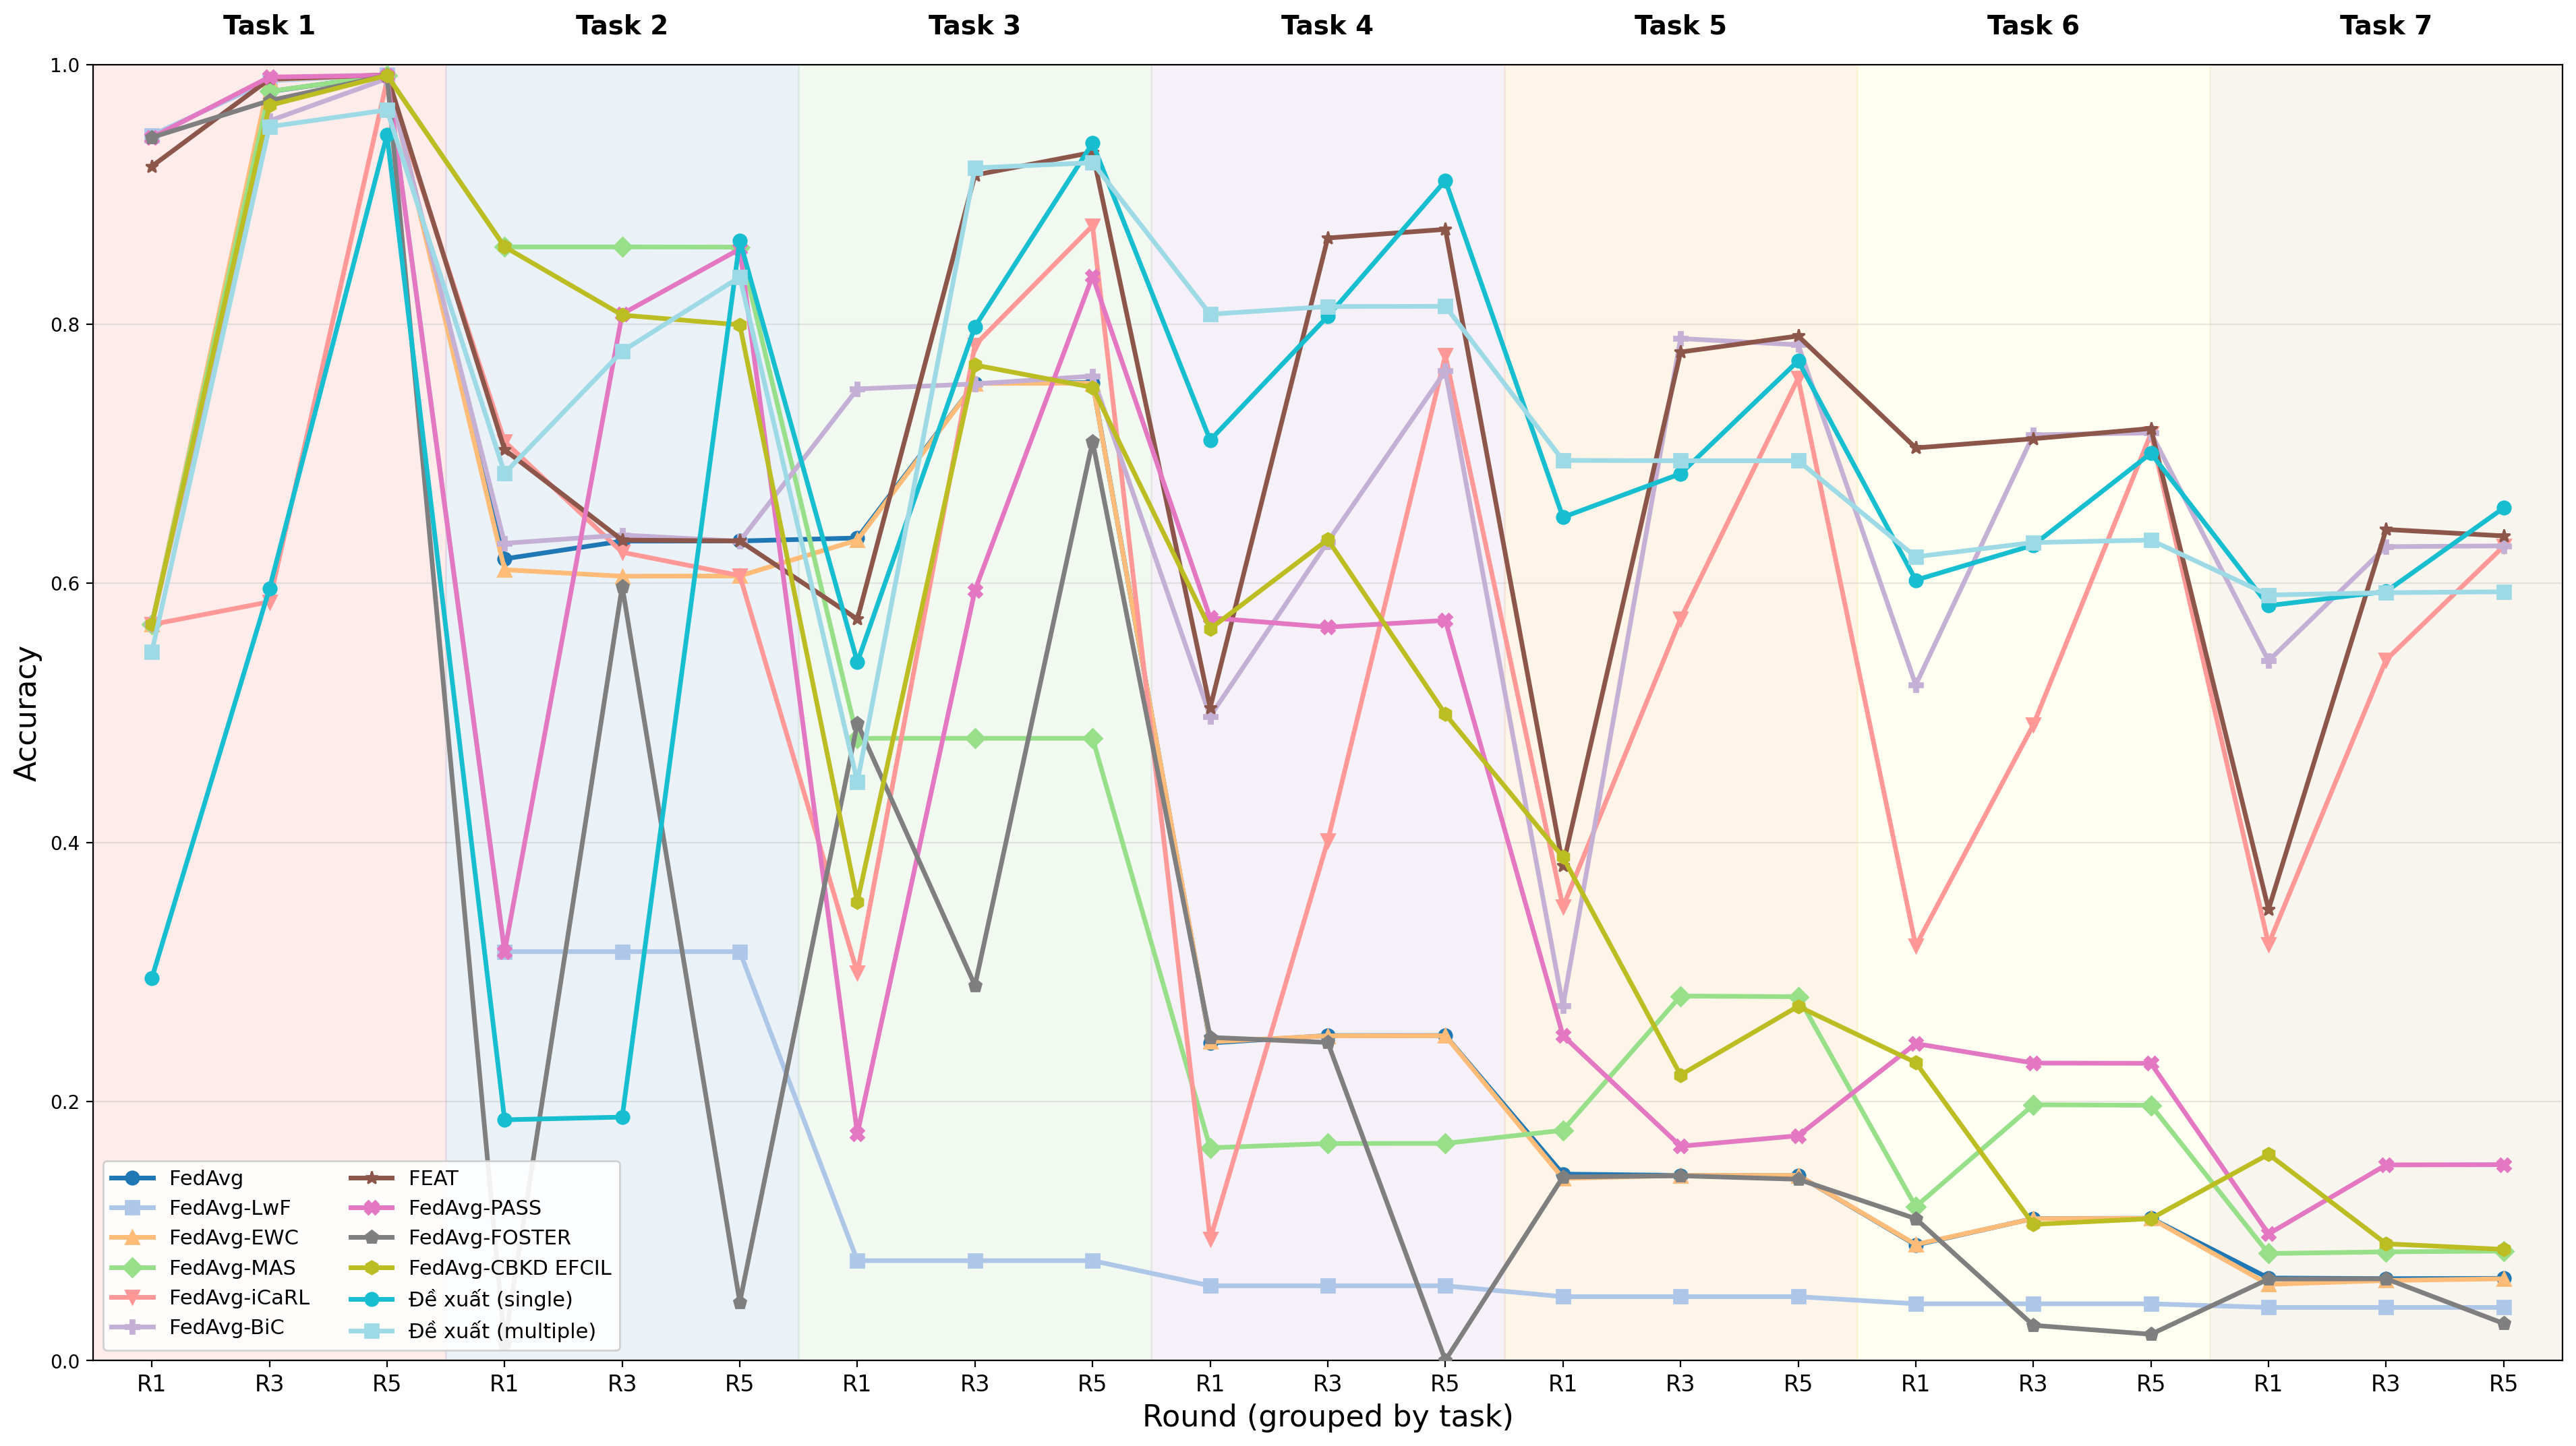
\includegraphics[width=1.0\textwidth]{images/OR_acc.png}
    \caption{Accuracy qua từng vòng liên kết của các phương pháp}
\label{fig:or_acc}
\end{figure*}

\begin{figure*}[ht]
    \centering
    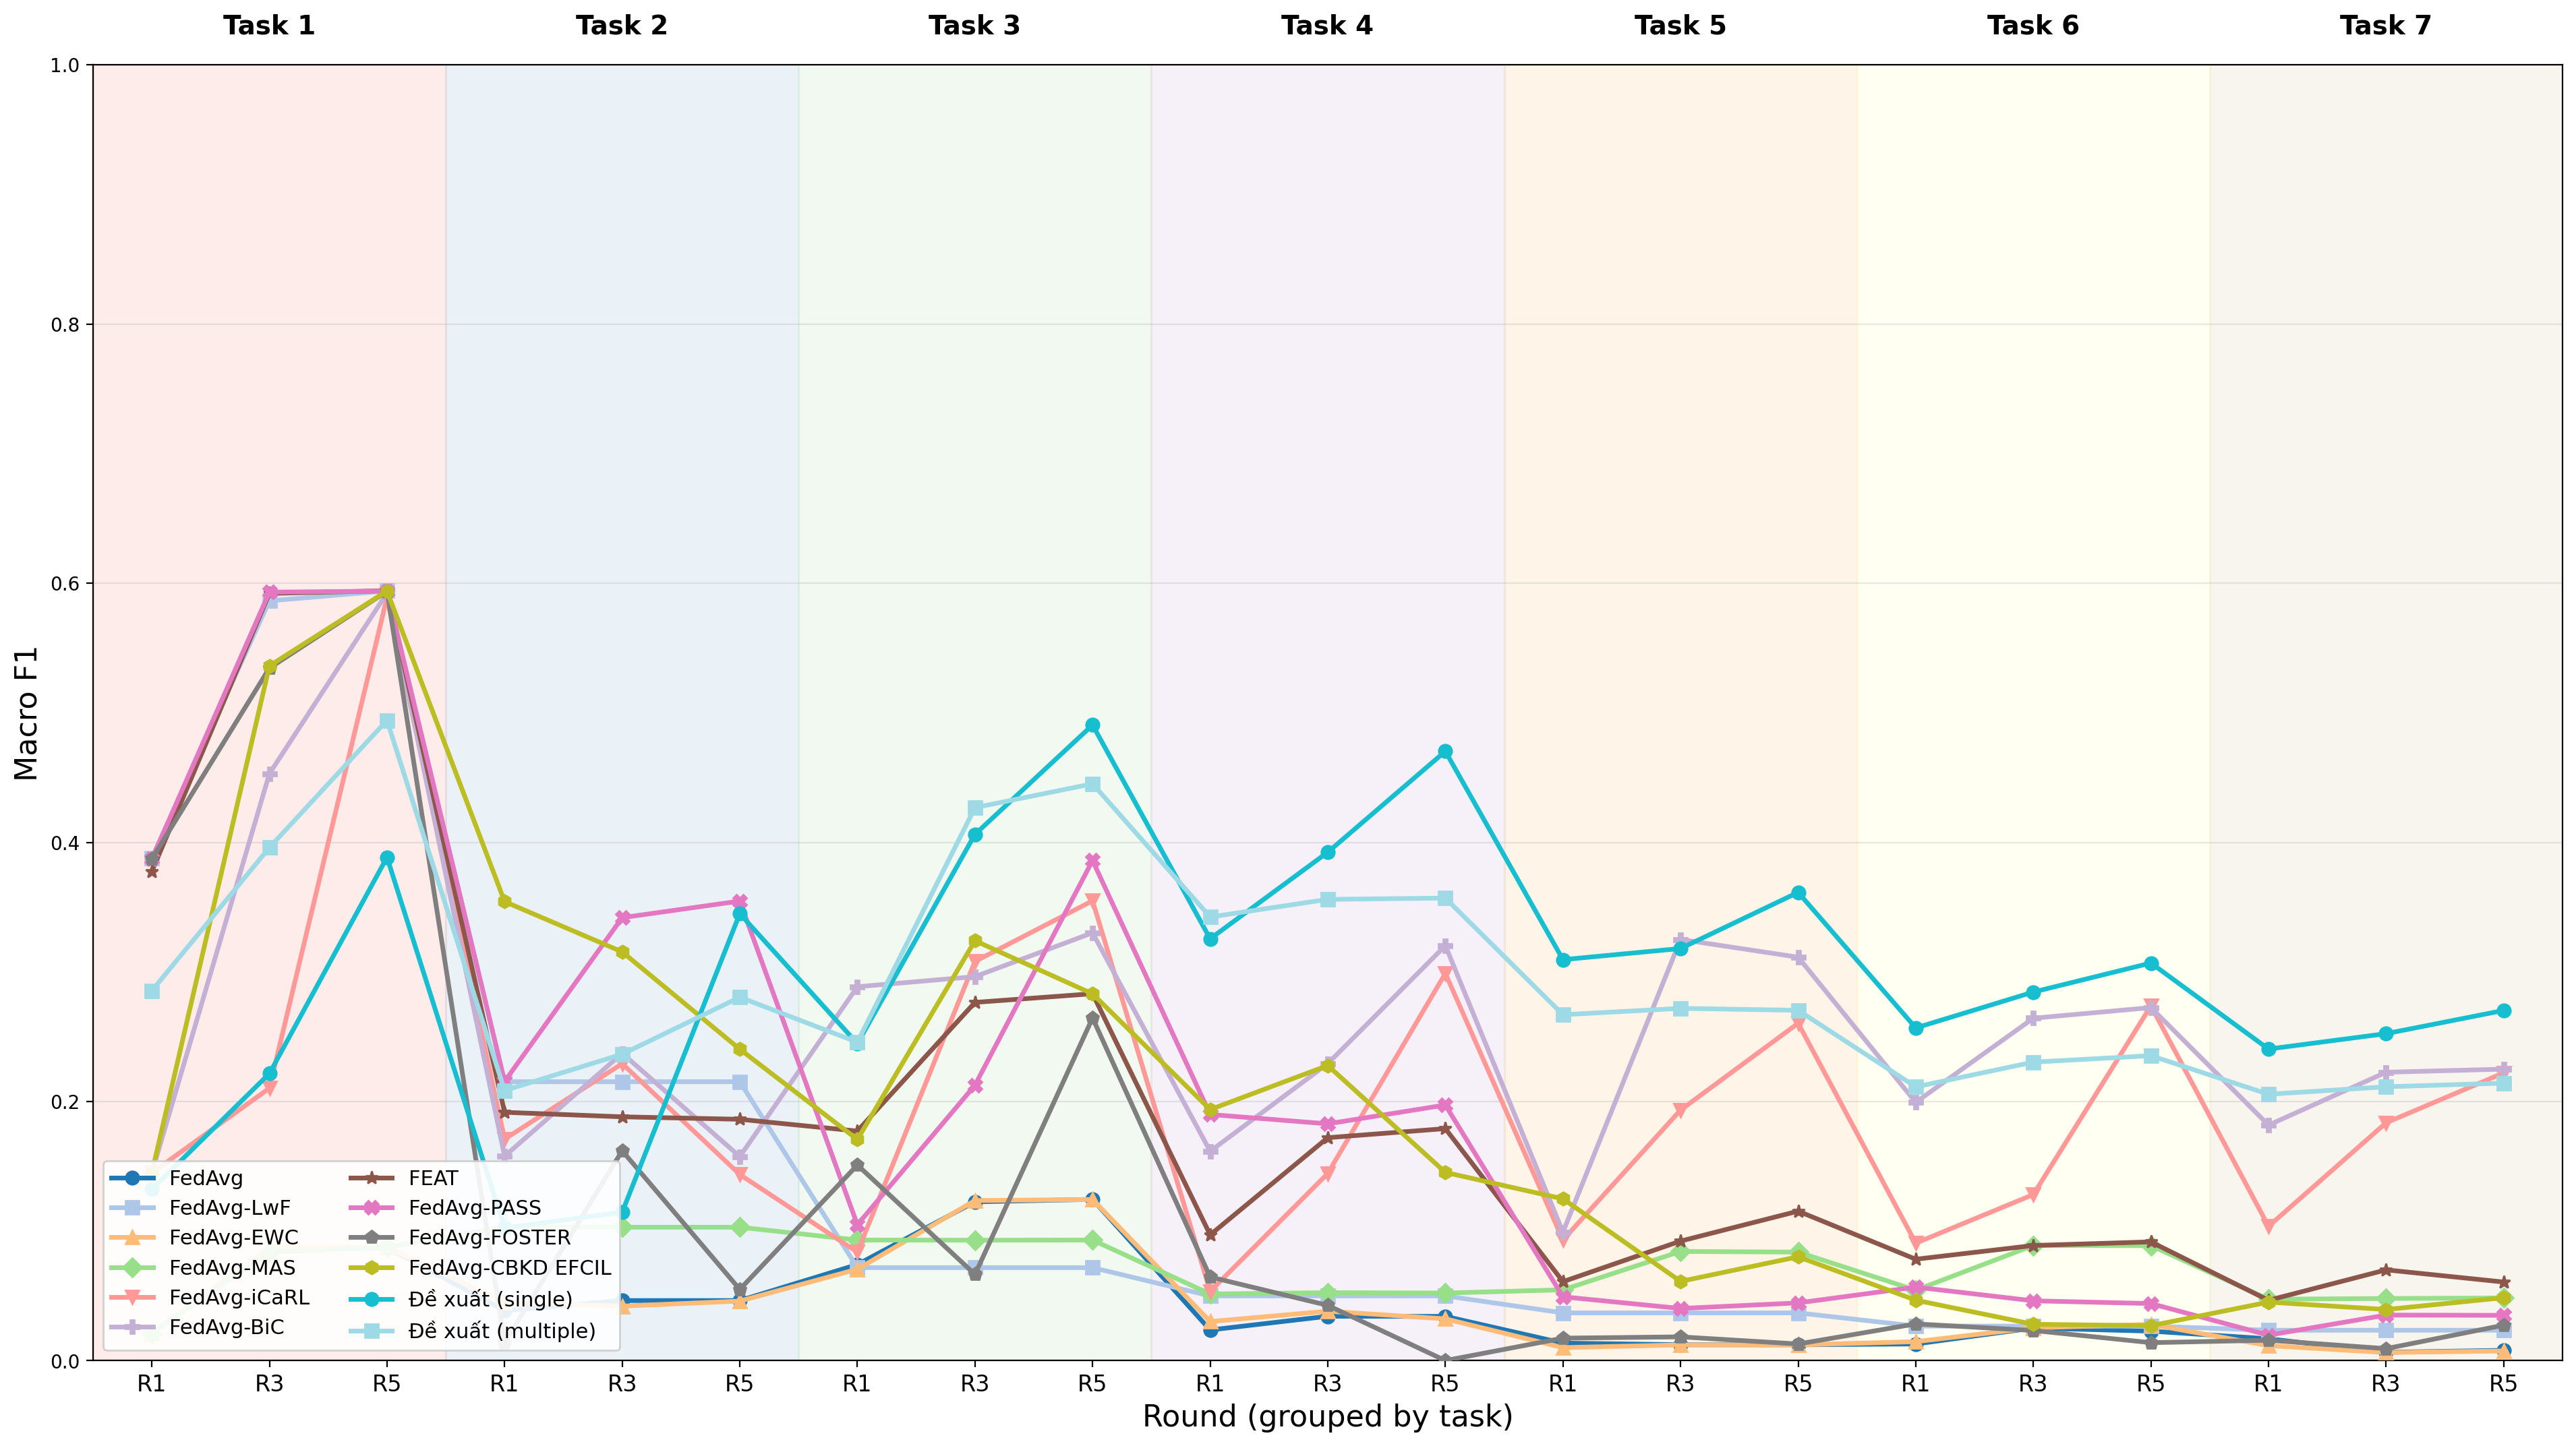
\includegraphics[width=1.0\textwidth]{images/OR_mf1.png}
    \caption{Macro F1 qua từng vòng liên kết của các phương pháp}
\label{fig:or_macf1}
\end{figure*}

\begin{figure*}[ht]
    \centering
    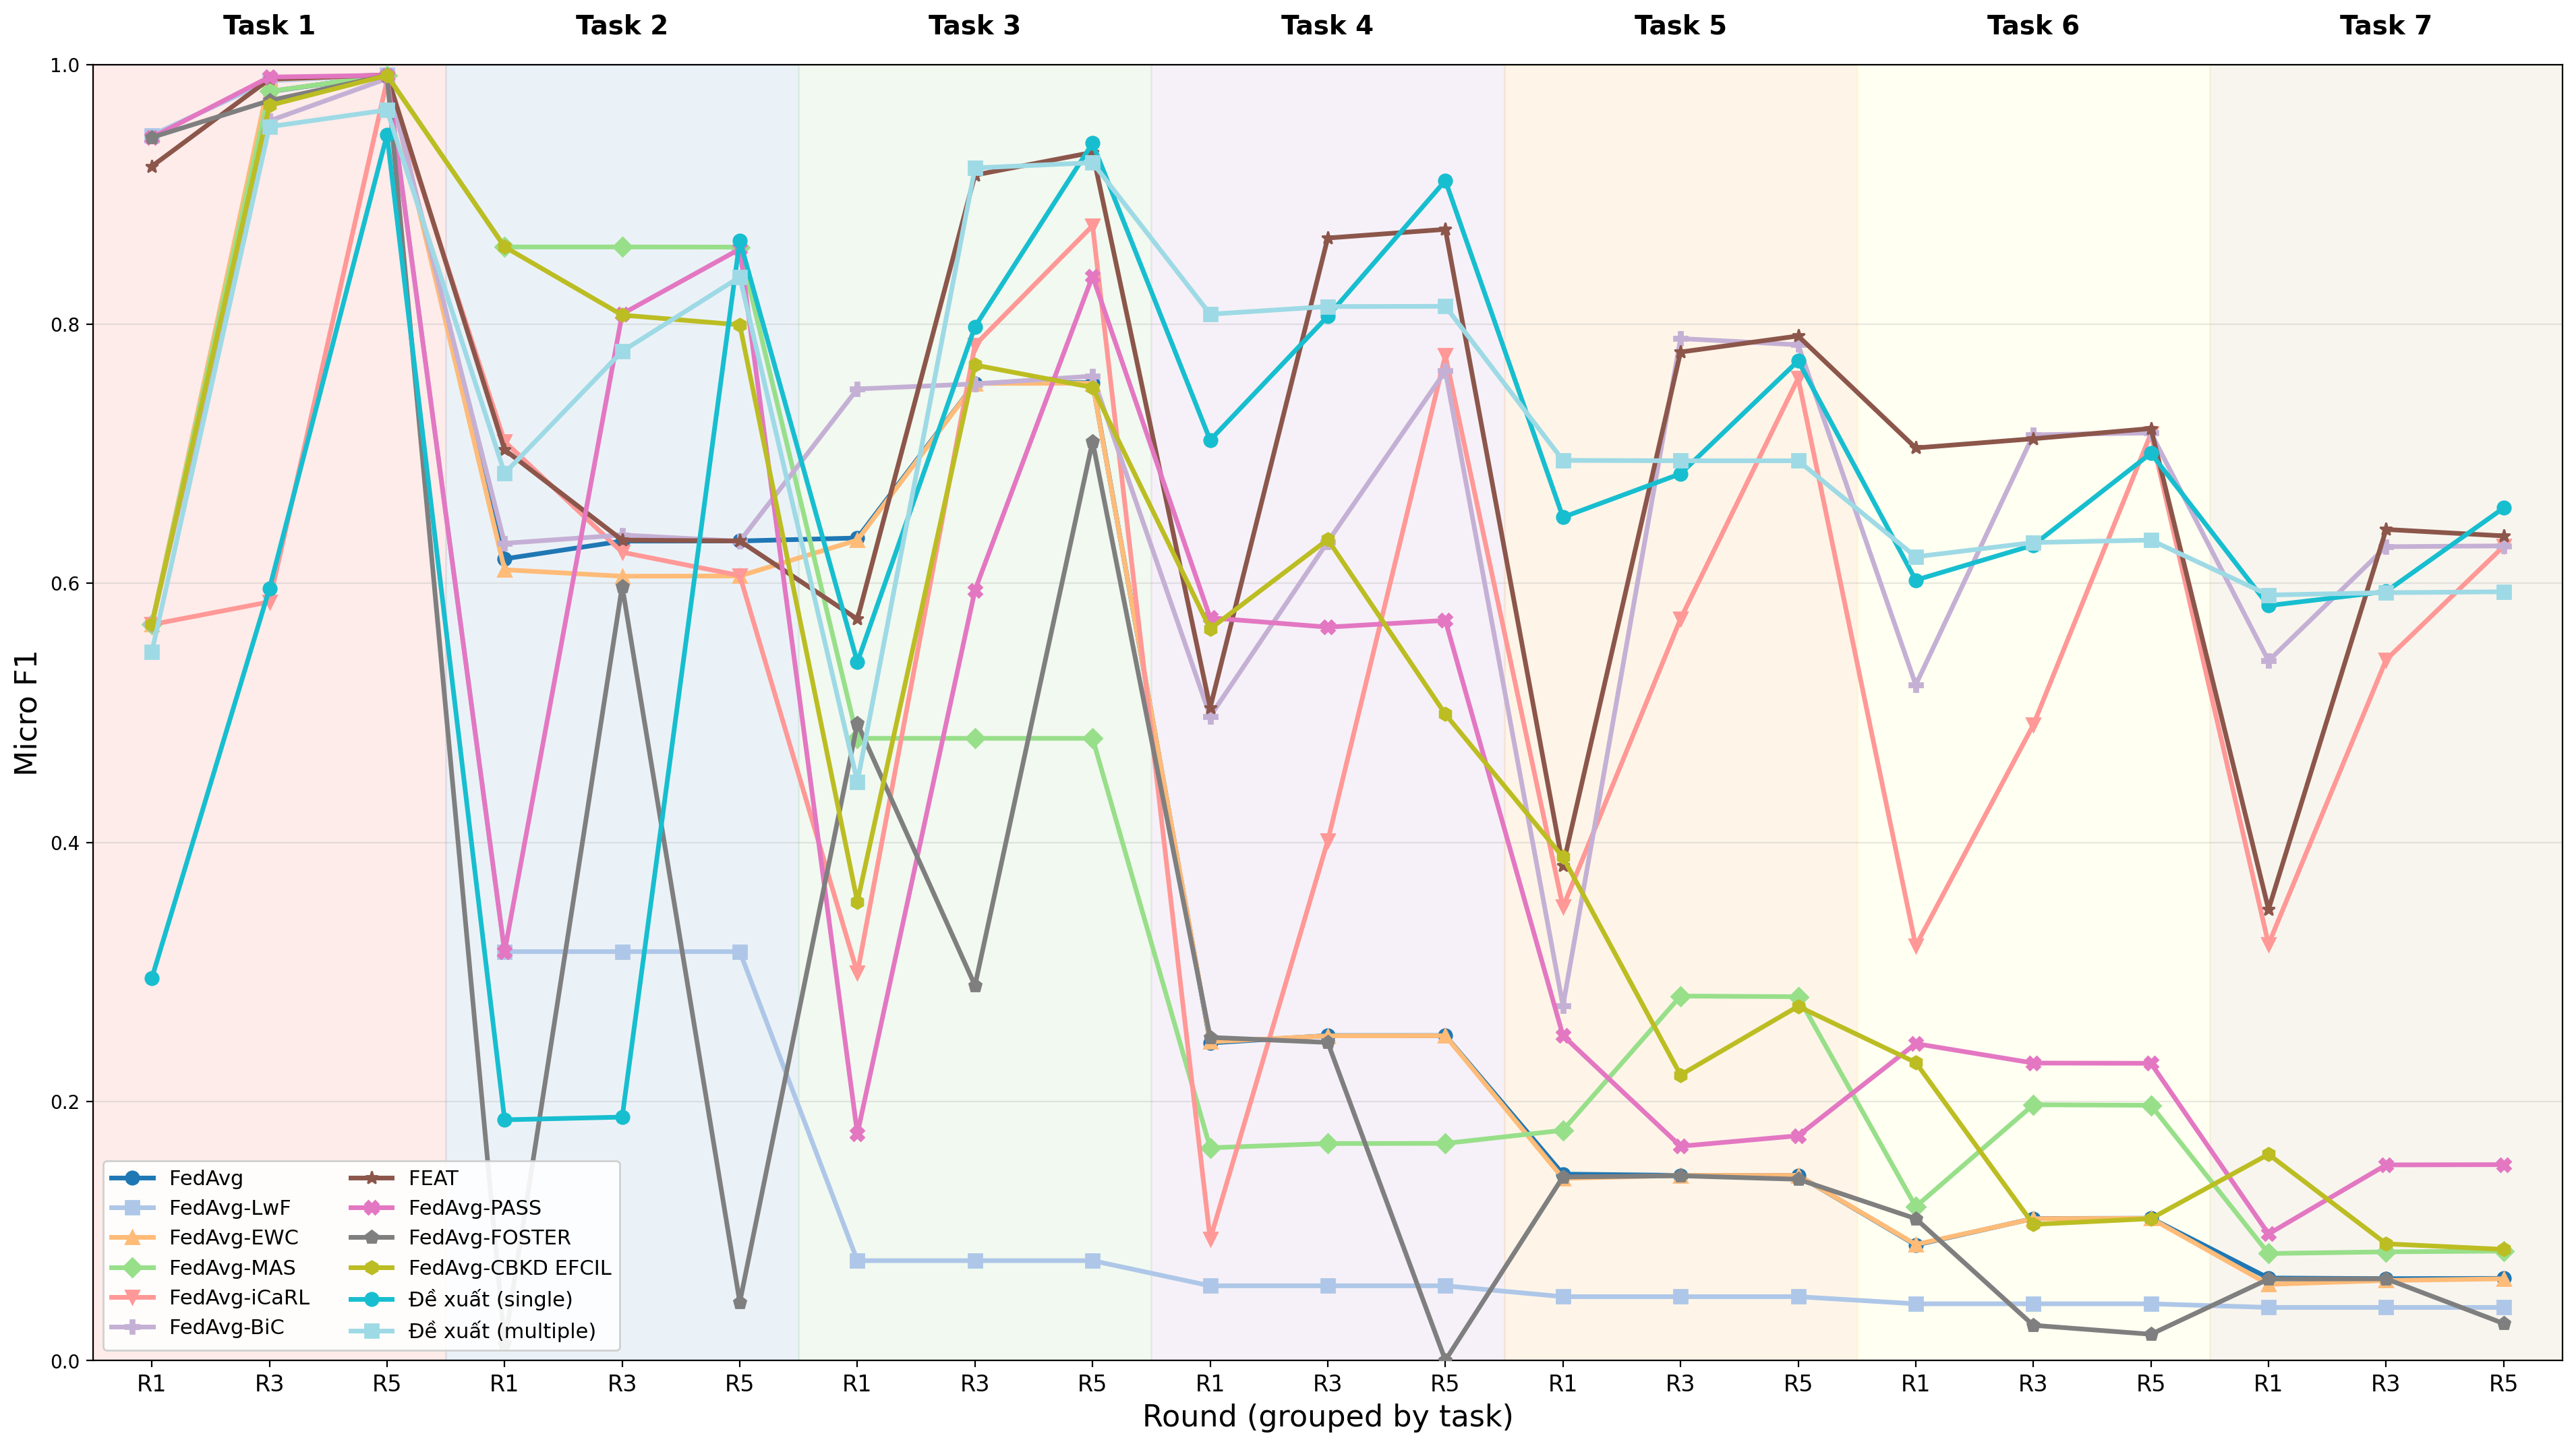
\includegraphics[width=1.0\textwidth]{images/OR_micf1.png}
    \caption{Micro F1 qua từng vòng liên kết của các phương pháp}
\label{fig:or_micf1}
\end{figure*}

\begin{figure*}[ht]
    \centering
    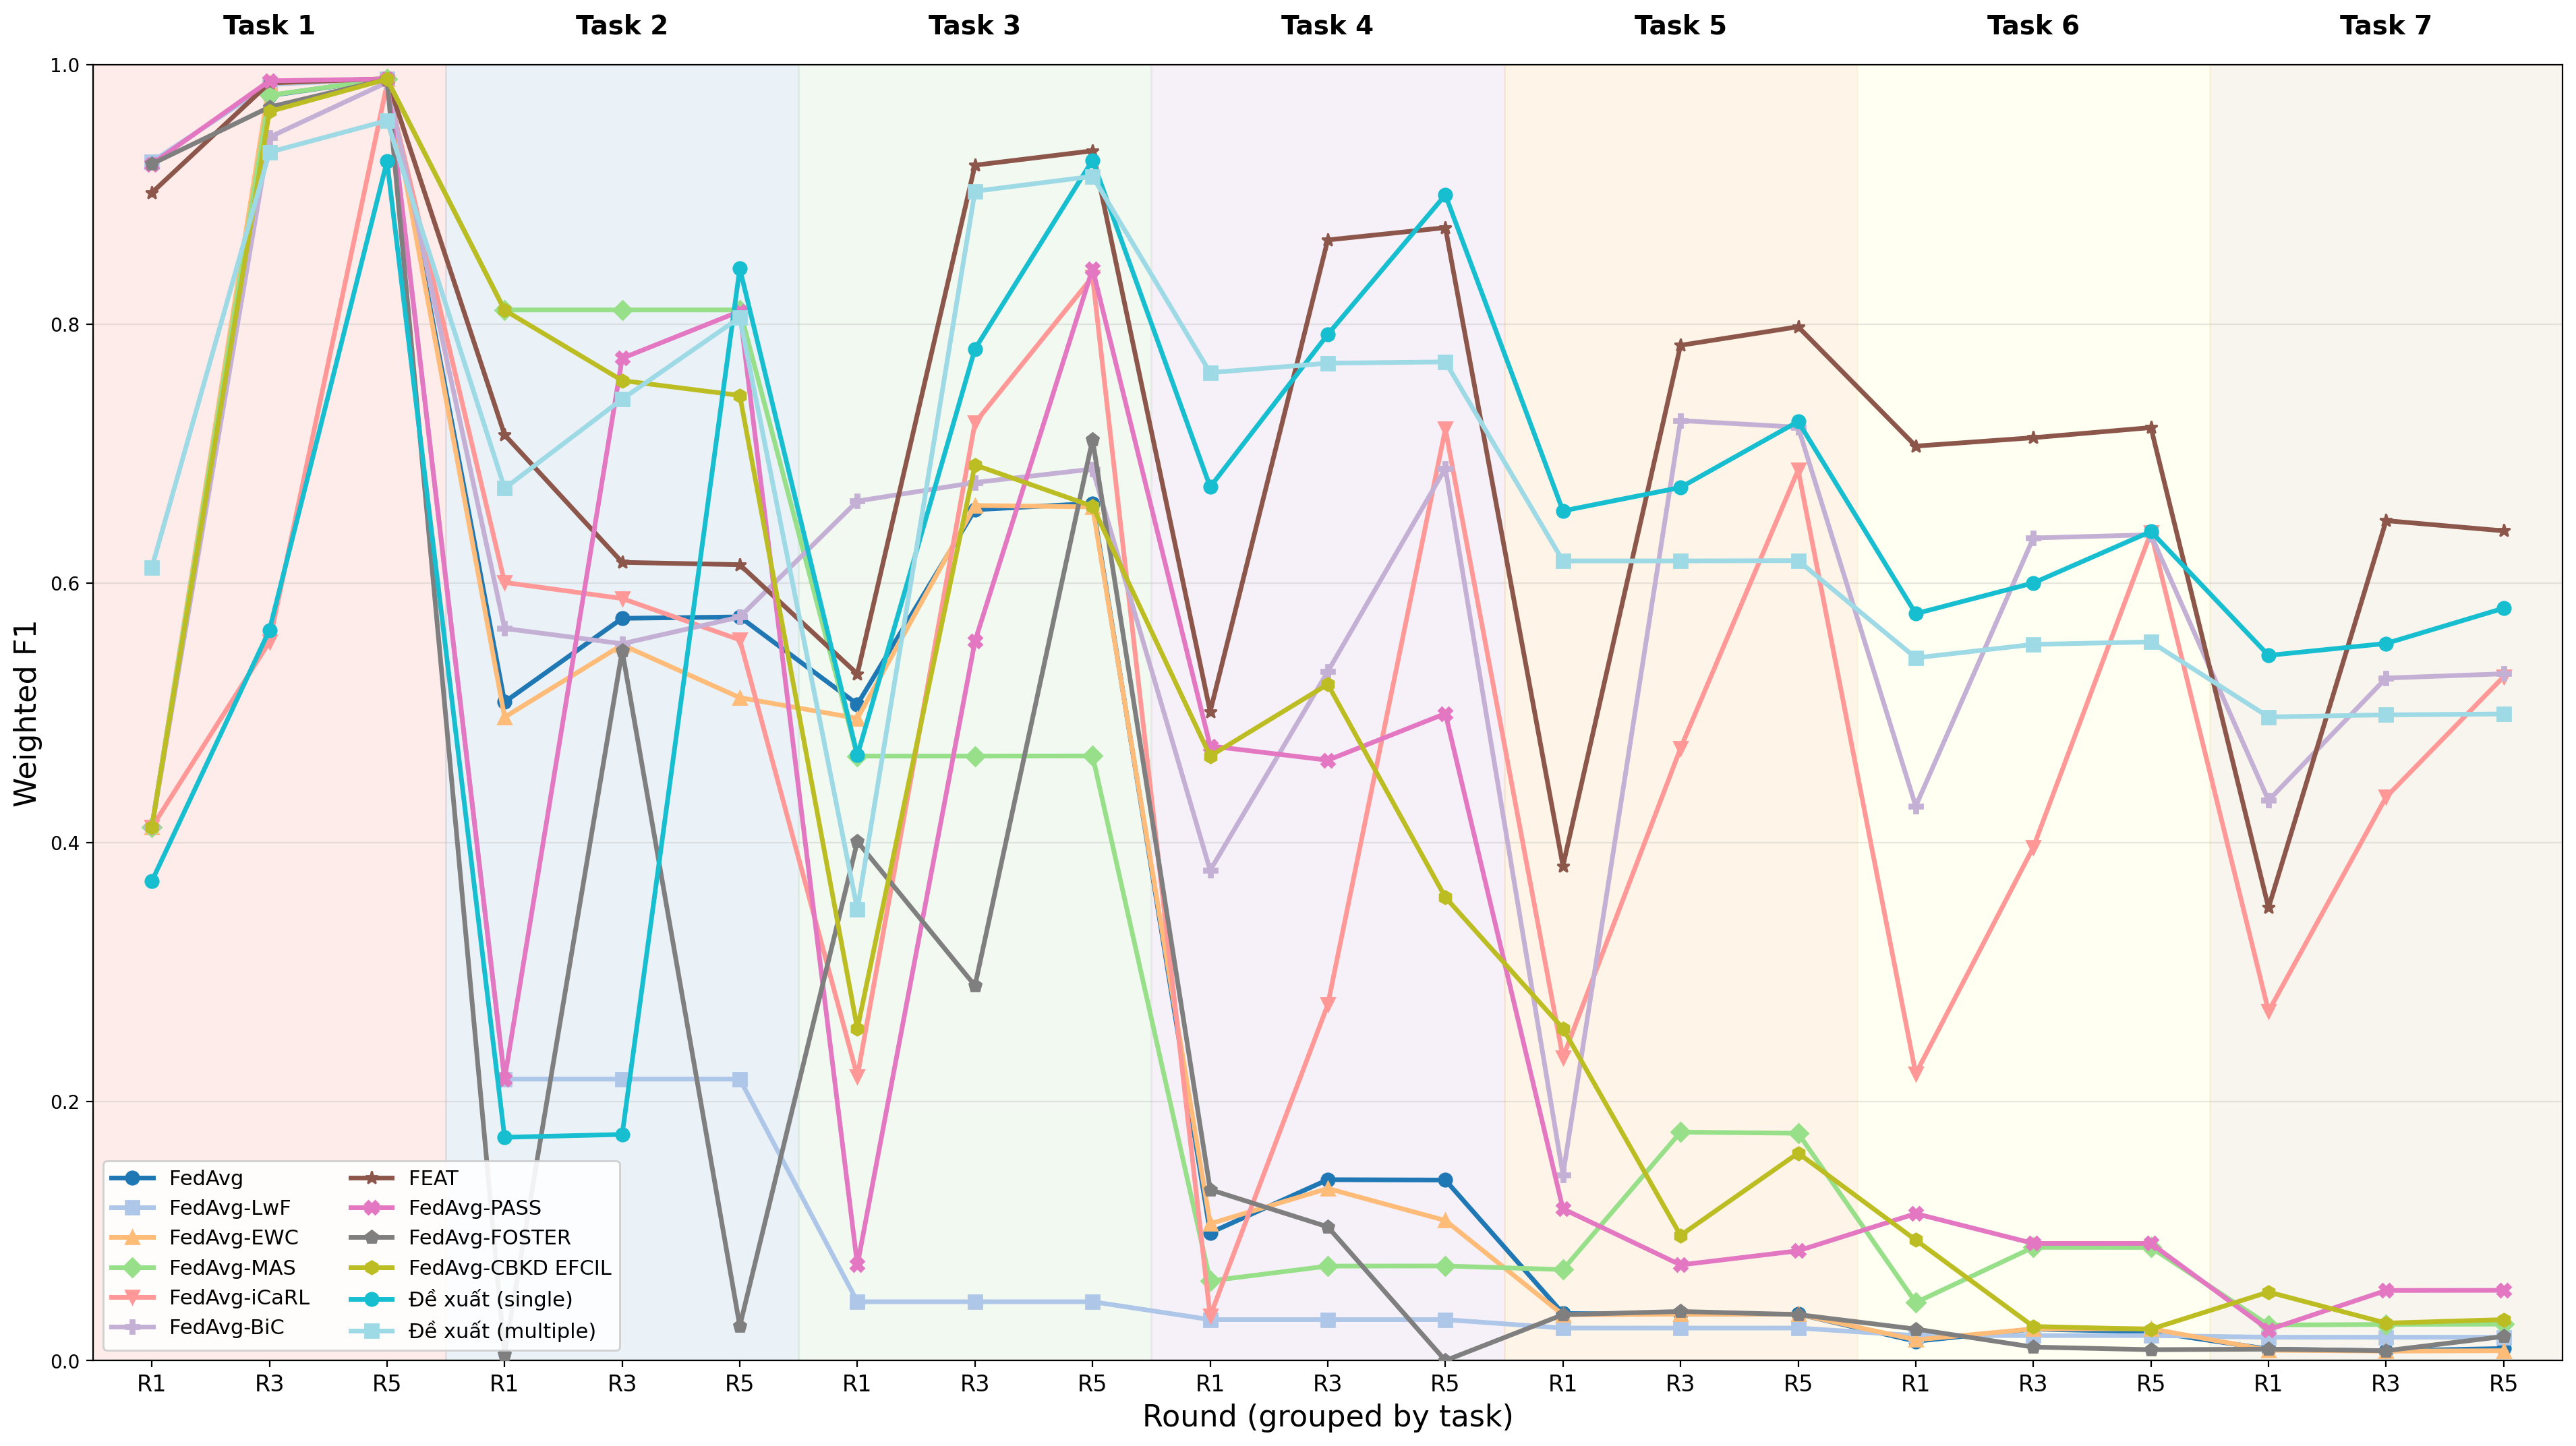
\includegraphics[width=1.0\textwidth]{images/OR_wf1.png}
    \caption{Weighted F1 qua từng vòng liên kết của các phương pháp}
\label{fig:or_wf1}
\end{figure*}

Bảng \ref{tab:cil_config} trình bày cấu hình của các thuật toán học tiệm tiến được đánh giá, bao gồm tham số ràng buộc, số mẫu được sử dụng để học tái diễn, và temperature chắt lọc.

\begin{table}[H]
    \centering
    \caption{Cấu hình các thuật toán học tiệm tiến.}
    \resizebox{\linewidth}{!}{
    \begin{tabular}{lcccc}
        \hline
        Thuật toán & Tham số & Số mẫu & Temperature & Ghi chú \\
        \hline
        FedAvg-EWC        & $\lambda=1000$ & - & - & Regularization \\
        FedAvg-MAS        & $\lambda=200$ & - & - & Regularization \\
        FedAvg-LwF        & $\alpha=0.99$ & - & $T=2$ & Regularization \\
        FedAvg-PASS       & $\lambda=10.0$, $\gamma=10.0$ & 1 \% & - & Prototype augment \\
        FedAvg-CBKD EFCIL & $\lambda=10.0$, $\alpha=10.0$, $\beta=10.0$ & 1 \% & - & Regularization \\
        FedAvg-iCaRL      & - & 1 \% & - & Replay \\
        FedAvg-BiC        & valid $=0.4$ & 1 \% & - & Replay \\
        %FEAT       & $\lambda=1.0$, $\rho=0.9$, $\tau=0.5$ & 1 \% & - & Replay \\
        FedAvg-FOSTER     & $\beta_1=0.97$, $\beta_2=0.97$ & 1 \% & - & Dynamic arch \\
        \hline
    \end{tabular}}
    \label{tab:cil_config}
\end{table}


\subsection{Thảo luận chung}

Chương này đã trình bày toàn bộ quá trình hiện thực và đánh giá phương pháp đề xuất trong môi trường học liên kết tiệm tiến lớp, đồng thời đặt phương pháp này trong tương quan với các hướng tiếp cận tiêu biểu của học tiệm tiến. Xét riêng về độ chính xác phân loại, phương pháp đề xuất chỉ đạt mức xấp xỉ so với các phương pháp replay-based như iCaRL, và sự chênh lệch này phản ánh đánh đổi có chủ đích trong thiết kế: thay vì tối ưu cực đại một chỉ số đơn lẻ, phương pháp hướng đến một tập hợp các tính chất hệ thống vốn ít được giải quyết đồng thời trong các nghiên cứu hiện có về học liên kết tiệm tiến lớp.

Trước hết, phương pháp đề xuất hỗ trợ học liên kết giữa các kiến trúc mô hình khác nhau (model heterogeneity), được được hiện thực (ký hiệu (multiple) trong bảng so sánh \ref{tab:cil_results_task6}) cho phép các client triển khai những mô hình hoàn toàn khác nhau mà vẫn cùng tham gia một quá trình học liên kết thống nhất. Xuyên suốt mọi task, hiệu quả phân loại của kịch bản đa kiến trúc mô hình liên tục tiệm cận các phương pháp đơn cấu trúc và thậm chí thuộc nhóm dẫn đầu ở một số task như task 2 với Accuracy tại task 2 ở $0.9245$, gần tương đương với FEAT ở $0.9325$, một phương pháp State-of-the-art đơn kiến trúc. Phương pháp trong kịch bản này cho thấy chỉ số Macro Precision cao thường xuyên dẫn đầu xuyên suốt 7 task học tiệm tiến. Đây là kết quả thực nghiệm khi có đến $25\%$ số client sử dụng mô hình nhỏ là CNN \ref{tab:cnn_arch}, và các mô hình không chỉ khác nhau về số đối mà còn khác nhau về mặt kiến trúc.

Ở kịch bản đơn kiến trúc, phương pháp đề xuất liên tục dẫn đầu so với các phương pháp khác, và luôn nằm ở mức tương đương so với FEAT. Điều này cho thấy hiệu quả học tiệm tiến rõ rệt của phương pháp đề xuất.

Tuy nhiên khác với FEAT, trong phương pháp đề xuất, do tri thức được trao đổi dưới dạng logits trên tập dữ liệu công khai thay vì trọng số mô hình, hệ thống đề xuất hoàn toàn tránh được các tấn công inference lên trọng số mô hình, giảm thiểu bề mặt của tấn công membership inference và hoàn toàn hỗ trợ được nhiều kiến trúc mô hình khác nhau trong quá trình học liên kết. Cùng với đó, cơ chế trao đổi dựa trên dữ liệu công khai mở ra khả năng triển khai phi tập trung mà không cần một máy chủ tổng hợp tham số trung tâm.

% Cuối cùng, phương pháp đề xuất cho phép điều chỉnh linh hoạt chi phí truyền thông. Bảng \ref{tab:comm_cost_cil} cho thấy các phương pháp dựa trên tham số như FedAvg luôn buộc client phải tải lên toàn bộ trọng số mô hình ở mỗi vòng, nên chi phí truyền thông bị cố định theo kích thước mô hình và không thể co giãn. Ngược lại, vì phương pháp đề xuất trao đổi logits trên dữ liệu công khai, lượng thông tin truyền đi tỉ lệ thuận với số mẫu công khai được chọn, nên người triển khai có thể chủ động đánh đổi giữa băng thông và chất lượng đồng thuận bằng cách điều chỉnh tỉ lệ dữ liệu công khai tham gia trao đổi. Tính co giãn này biến chi phí truyền thông từ một ràng buộc cứng thành một tham số thiết kế có thể tinh chỉnh theo điều kiện hạ tầng cụ thể của từng bên tham gia.

Như vậy, khóa luận này đã thành công trình bày một hệ thống học máy liên kết cho phát hiện xâm nhập có tính ứng dụng thực tiễn cao và đồng thời giải quyết được các khó khăn cũng như điểm yếu của những hệ thống học liên kết truyền thống, với hiệu suất hoạt động cạnh tranh cao với các thuật toán học tiệm tiến hiện đại.
\chapter{KẾT LUẬN VÀ HƯỚNG PHÁT TRIỂN}\label{Chapter5}

\section*{Tóm tắt chương}

Chương này tổng kết nội dung khóa luận, nêu các đóng góp chính và đề xuất hướng phát triển tiếp theo cho hệ thống Decentralized Federated Distillation kết hợp Class-Incremental Learning.

\section{Kết luận}

Khóa luận đã trình bày một cơ chế học liên kết hỗ trợ học liên kết giữa các kiến trúc mô hình khác nhau (model heterogeneity), được được hiện thực (ký hiệu (multiple) trong bảng so sánh \ref{tab:cil_results_task6}) cho phép các client triển khai những mô hình hoàn toàn khác nhau mà vẫn cùng tham gia một quá trình học liên kết thống nhất. Xuyên suốt mọi task, hiệu quả phân loại của kịch bản đa kiến trúc mô hình liên tục tiệm cận các phương pháp đơn cấu trúc và thậm chí thuộc nhóm dẫn đầu ở một số task như task 2 với Accuracy tại task 2 ở $0.9245$, gần tương đương với FEAT ở $0.9325$, một phương pháp State-of-the-art đơn kiến trúc. Phương pháp trong kịch bản này cho thấy chỉ số Macro Precision cao thường xuyên dẫn đầu xuyên suốt 7 task học tiệm tiến. Đây là kết quả thực nghiệm khi có đến $25\%$ số client sử dụng mô hình nhỏ là CNN \ref{tab:cnn_arch}, và các mô hình không chỉ khác nhau về số đối mà còn khác nhau về mặt kiến trúc.

Ở kịch bản đơn kiến trúc, phương pháp đề xuất liên tục dẫn đầu so với các phương pháp khác, và luôn nằm ở mức tương đương so với FEAT. Điều này cho thấy hiệu quả học tiệm tiến rõ rệt của phương pháp đề xuất.

Tuy nhiên khác với FEAT, trong phương pháp đề xuất, do tri thức được trao đổi dưới dạng logits trên tập dữ liệu công khai thay vì trọng số mô hình, hệ thống đề xuất hoàn toàn tránh được các tấn công inference lên trọng số mô hình, giảm thiểu bề mặt của tấn công membership inference và hoàn toàn hỗ trợ được nhiều kiến trúc mô hình khác nhau trong quá trình học liên kết. Cùng với đó, cơ chế trao đổi dựa trên dữ liệu công khai mở ra khả năng triển khai phi tập trung mà không cần một máy chủ tổng hợp tham số trung tâm.

Thực nghiệm của hệ thống cho thấy độ chính xác cao, vượt qua nhiều phương pháp học tiệm tiến trong khi giải quyết nhiều khó khăn thực tế của các hệ thống học máy liên kết. Bằng cách ứng dụng phương pháp học tiệm tiến dựa trên tái diễn dữ liệu và kiến trúc dynamic, cũng như nhiều kỹ thuật tiên tiến có chi phí thấp như EVA và EKD, khóa luận đã thành công trình bày một hệ thống mang tính thực tiễn với độ hiệu quả cao cho bài toán học liên kết phát hiện xâm nhập.

\section{Đóng góp chính}

\begin{itemize}
    \item \textbf{Hệ thống học liên kết phân tán dựa trên học chắt lọc kết hợp học tiệm tiến theo nhãn}: Khóa luận đã xây dựng một hệ thống hoàn chỉnh cho phép mô phỏng và đánh giá các phương pháp học liên kết trong ngữ cảnh học tiệm tiến lớp, so sánh với $9$ phương pháp học tiệm tiến của cả ba loại: dựa trên ràng buộc (regularization), tái diễn dữ liệu (replay/exemplar rehearsal), và kiến trúc dynamic (dynamic architecture) cùng phương pháp đề xuất dựa trên chắt lọc liên kết. Hệ thống được hiện thực chủ yếu trên PyTorch với khả năng chuyển đổi linh hoạt giữa hai backend TensorFlow và PyTorch, hỗ trợ cả kịch bản đơn kiến trúc và đa kiến trúc, đồng thời cung cấp cơ chế checkpoint để phục hồi sau sự cố trong quá trình huấn luyện kéo dài, file log chi tiết với mốc đo thời gian.
    
    \item \textbf{Phương pháp đề xuất}: Phương pháp đề xuất đã giải quyết được nhiều khó khăn mang tính thực tiễn cao: khả năng hỗ trợ kiến trúc mô hình khác nhau, cải thiện bảo mật dữ liệu trước các tấn công suy ngược mô hình và gây khó khăn nhiều hơn cho các kiểu tấn công membership inference trong khi vẫn giữ được khả năng phân loại tiệm cận hoặc cao hơn các phương pháp học tiệm tiến State-of-the-art như FEAT.
    
    % \item \textbf{Chi phí truyền thông co giãn được}: Phương pháp đề xuất đã biến chi phí truyền thông từ một ràng buộc cứng thành một tham số thiết kế có thể tinh chỉnh. Thay vì buộc client phải tải lên toàn bộ trọng số mô hình ở mỗi vòng như các phương pháp dựa trên tham số, phương pháp đề xuất trao đổi logits trên dữ liệu công khai với lượng thông tin tỉ lệ thuận với số mẫu công khai được chọn, cho phép người triển khai chủ động đánh đổi giữa băng thông và chất lượng đồng thuận.
    
    \item \textbf{Đánh giá thực nghiệm toàn diện trên CICIoT2023}: Khóa luận đã tiến hành đánh giá thực nghiệm toàn diện trên tập dữ liệu CICIoT2023 với $34$ lớp tấn công phân bố trên $7$ task nối tiếp, trong đó số lượng client tăng dần từ $40$ lên $100$ để mô phỏng quá trình mở rộng mạng lưới IDS liên kết. Kết quả thực nghiệm đã làm rõ khả năng của từng phương pháp trong việc học tiệm tiến tiếp nhận các lớp tấn công mới mà vẫn duy trì tri thức đã học, .
\end{itemize}

\section{Hướng phát triển}

Bên cạnh các khó khăn đã được giải quyết hiệu quả bằng phương pháp đề xuất, khóa luận vẫn còn nhiều không gian phát triển để minh chứng và cải thiện tốt hơn tính ứng dụng:

\begin{itemize}
    % \item \textbf{Triển khai trên hệ thống IDS thực tế}: Hướng phát triển ưu tiên hàng đầu là đưa hệ thống từ môi trường mô phỏng vào triển khai thực tế trên các hệ thống phát hiện xâm nhập trong doanh nghiệp hoặc tổ chức. Việc này đòi hỏi giải quyết các thách thức về tích hợp với hạ tầng mạng hiện có, xử lý lưu lượng mạng thời gian thực với độ trễ thấp, và đảm bảo khả năng mở rộng khi số lượng client và lớp tấn công tăng lên. Thử nghiệm trên môi trường thực tế cũng sẽ cung cấp dữ liệu đánh giá phong phú hơn, bao gồm các kiểu tấn công mới nổi và phân phối dữ liệu phức tạp hơn so với tập dữ liệu CICIoT2023.
    
    \item \textbf{Tích hợp với hệ thống SIEM/SOC}: Hệ thống có thể được tích hợp với các hệ thống Security Information and Event Management (SIEM) hoặc Security Operations Center (SOC) để cung cấp khả năng phát hiện xâm nhập phân tán và thích nghi theo thời gian. Trong kịch bản này, mỗi tổ chức tham gia sẽ vận hành một client của hệ thống, và tri thức về các kiểu tấn công mới được chia sẻ thông qua cơ chế chắt lọc liên kết mà không làm lộ dữ liệu nhạy cảm. Việc tích hợp này cũng đòi hỏi phát triển giao diện người dùng trực quan để các nhà phân tích bảo mật có thể theo dõi hiệu năng của mô hình, điều tra các cảnh báo sai, và cập nhật chính sách phản ứng tự động.
    
    % \item \textbf{Kiểm chứng thực nghiệm khả năng phi tập trung}: Mặc dù phương pháp đề xuất đã được phân tích ở mức lý thuyết về khả năng triển khai phi tập trung, việc kiểm chứng thực nghiệm vẫn chưa được thực hiện. Hướng phát triển tiếp theo là xây dựng một kiến trúc mạng ngang hàng (peer-to-peer) cho phép các client trao đổi logits trực tiếp mà không cần máy chủ trung tâm, đồng thời đánh giá hiệu năng của hệ thống trong các điều kiện mạng không ổn định, độ trễ cao, và một số client có thể rời khỏi hoặc gia nhập hệ thống bất cứ lúc nào.
    
    \item \textbf{Gia tăng hiệu năng}: Mặc dù phương pháp đề xuất đã đạt được các tính chất hệ thống mong muốn, độ chính xác phân loại xét riêng trong việc phát hiện các nhãn tấn công vẫn còn đạt hiệu quả trung bình, khi các mô hình chỉ phát hiện được các tấn công thường thấy (như tấn công DDoS) mà lại phân loại kém hơn trên các kiểu tấn công hiếm (XSS, Dictionary Brute Forcing,...), dẫn tới chỉ số Macro F1 còn chưa tối ưu. Đây là một vấn đề sinh ra từ đặc tính mất cân bằng nhãn rất cao của tập dữ liệu CICIoT23, và giải quyết vấn đề này là một hướng phát triển hoàn toàn cần thiết của khóa luận này.
    
    % \item \textbf{Đánh giá trên nhiều tập dữ liệu IDS khác}: Để khẳng định tính tổng quát của hệ thống, cần tiến hành đánh giá trên nhiều tập dữ liệu phát hiện xâm nhập khác nhau, bao gồm các tập dữ liệu với đặc trưng mạng đa dạng hơn (ví dụ: NSL-K, UNSW-NB15, CSE-CIC-IDS2018) và các kịch bản tấn công phức tạp hơn (ví dụ: tấn công zero-day, tấn công đa giai đoạn). Việc này cũng sẽ giúp xác định các trường hợp sử dụng phù hợp nhất cho từng phương pháp học tiệm tiến.
    
    % \item \textbf{Tối ưu chi phí truyền thông và tính toán}: Mặc dù phương pháp đề xuất đã cho phép điều chỉnh linh hoạt chi phí truyền thông, việc tối ưu hóa cả chi phí truyền thông lẫn chi phí tính toán ở phía client vẫn là một hướng nghiên cứu quan trọng. Các kỹ thuật như lượng tử hóa logits, nén dữ liệu công khai, và học tăng cường để tự động điều chỉnh tỉ lệ dữ liệu công khai theo điều kiện mạng có thể được khám phá để giảm thiểu tổng chi phí vận hành.
    
    \item \textbf{Bổ sung phân tích khả giải cho dự đoán IDS}: Trong bối cảnh ứng dụng vào phát hiện xâm nhập, khả năng giải thích dự đoán của mô hình có vai trò quan trọng để các nhà phân tích bảo mật có thể hiểu được lý do đằng sau các cảnh báo và đưa ra quyết định phản ứng phù hợp. Hướng phát triển này bao gồm việc tích hợp các kỹ thuật như SHAP, LIME, hoặc attention visualization vào hệ thống, qua đó cung cấp thông tin chi tiết về các đặc trưng quan trọng nhất trong việc phân loại từng kiểu tấn công.
    
    \item \textbf{Hoàn thiện cơ chế chống tấn công poisoning}: Trong môi trường thực tế, một số client có thể bị xâm nhập hoặc hoạt động bất thường (Byzantine actors), dẫn đến việc gửi thông tin sai lệch cho hệ thống. Hướng phát triển tiếp theo là hoàn thiện tích hợp một cơ chế phát hiện và cách ly client bất thường, đồng thời thiết kế các giao thức đồng thuận bền vững trước các kiểu tấn công nhằm vào kiến trúc phân tán như Free-rider attack hay Sybil attack \cite{douceur2002sybil}
\end{itemize}


\printbibliography[title={TÀI LIỆU THAM KHẢO}]
\addcontentsline{toc}{chapter}{\textbf{TÀI LIỆU THAM KHẢO}}

\end{document}
